\documentclass[a4j,10.5pt,dvipdfmx]{jsreport}

% ----- 仕掛け 開始 -----
\newcommand{\ifdraft}{false}
\newcommand{\ismain}{} 
% ----- 仕掛け 終了 -----

% 数式
\usepackage{amsmath,amsfonts}
\usepackage{bm}

% 画像
\usepackage[top=35truemm,bottom=30truemm,left=30truemm,right=30truemm]{geometry}
\usepackage[dvipdfmx]{graphicx}

% biblatex
\usepackage[style=numeric, sorting=none, maxbibnames=1000]{biblatex}
\addbibresource{master_thesis.bib}

% itembox
\usepackage{ascmac}
\usepackage{itembkbx}

% フォント
\usepackage[ipaex]{pxchfon}

\usepackage{float}
\usepackage{multicol}
\usepackage{multirow}
\usepackage{paralist}
\usepackage{caption}
\captionsetup[figure]{font=small}
\captionsetup[table]{font=small}
\captionsetup{format=hang}

% 行間設定
\usepackage{setspace}
\setstretch{1.25}

\usepackage{algorithm}
\usepackage{algpseudocode}
\usepackage[dvipdfmx,
    colorlinks=true,       % 色付けを有効にする
    linkcolor=blue,        % 目次・図表リンクなど（青）
    citecolor=green,       % 参考文献の引用 [1] など（緑）
    urlcolor=blue,         % URL（青 ※ここも緑がよければ green に）
    bookmarks=true,        % しおり（PDFの目次）を作成
    bookmarksnumbered=true % しおりに番号を入れる
]{hyperref}
\usepackage{pxjahyper}
\usepackage{fancyhdr}
\usepackage{capt-of}
\usepackage{tabularx}
\usepackage{enumitem}
\usepackage{threeparttable}
\usepackage{booktabs}
\usepackage{titlesec} % titlesec必須
\usepackage[export]{adjustbox} 
\usepackage{docmute} 
\usepackage{makecell}
\usepackage{forest}
\usepackage{fancybox}
\usepackage{longtable}
\usepackage{xltabular}

% paragraphの設定
\titleformat{\paragraph}[runin]
  {\normalfont\normalsize\bfseries}
  {}{0pt}{}
\titlespacing*{\paragraph}
  {0pt}{1.0ex}{0.8em}

% Chapterの設定
\titleformat{\chapter}[hang]{\LARGE\bfseries}{{\Large \prechaptername\thechapter\postchaptername}}{1em}{}

\setlength{\headheight}{16.5pt}
\setcounter{tocdepth}{2}

% =========================================================
% ▼▼▼ ヘッダー・フッターの決定版設定 ▼▼▼

% 1. 基本設定（通常ページ用）
\pagestyle{fancy}
\fancyhf{} % 一度クリア

% ヘッダー：左に章、右に節
\lhead{\leftmark}  
\rhead{\rightmark} 
% フッター：中央下にページ番号
\cfoot{\thepage}

\renewcommand{\headrulewidth}{0.4pt} % 線の太さ

% 章・節タイトルの表示形式
\renewcommand{\chaptermark}[1]{\markboth{第\ \thechapter\ 章\ #1}{}}
\renewcommand{\sectionmark}[1]{\markright{\thesection\ #1}{}}

% 2. 章の始まり専用のスタイル「chapterstart」を定義
\fancypagestyle{chapterstart}{
   \fancyhf{}       % ヘッダー・フッターを空にする
   \cfoot{\thepage} % ページ番号を中央下に配置
   \renewcommand{\headrulewidth}{0pt} % 線なし
}

% 3. titlesecの機能で「章の始まりはこのスタイルを使え」と命令
\assignpagestyle{\chapter}{chapterstart}

% ▲▲▲▲▲▲▲▲▲▲▲▲▲▲▲▲▲▲▲▲▲▲▲▲▲▲▲▲▲
% =========================================================

\begin{document}

%rename
\renewcommand{\abstractname}{\LARGE 論文要旨}

% タイトルページ
\begin{titlepage}
   \noindent
   {\Large 修士論文} \hfill {\Large 2025年度}

   \vspace*{70truept}

   \begin{center}
      \vspace{60truept}
      {\Huge \bfseries 脚本に基づく漫画のネーム生成} \par

      \vspace{110truept}

      {\LARGE 渡邉 謙吾} \par
      \vspace{5truept}
      {\LARGE （学籍番号：82420611）} \par

      \vspace{110truept}

      {\LARGE 指導教員 教授 栗原 聡} \par

      \vspace{50truept}

      {\Large 2026 年 3 月 } \par

      \vspace{50truept}

      {\Large 慶應義塾大学大学院理工学研究科} \par
      \vspace{10truept}
      {\Large 開放環境科学専攻} \par
   \end{center}
\end{titlepage}

% 概要
\documentclass[a4j,10.5pt,dvipdfmx]{jsreport}

% 数式
\usepackage{amsmath,amsfonts}
\usepackage{bm}

% 画像
\usepackage[dvipdfmx,top=35truemm,bottom=30truemm,left=30truemm,right=30truemm]{geometry}
\usepackage[dvipdfmx]{graphicx}
% biblatex
\usepackage[style=numeric, sorting=none, maxbibnames=1000]{biblatex}
\addbibresource{graduation_thesis.bib}

% itembox
\usepackage{ascmac}
% breakitemboxのためのpackage
\usepackage{itembkbx}
% \usepackage{tcolorbox} 画像が見えなくなってしまう原因
% \usepackage{framed} 枠

% フォント
\usepackage[ipaex]{pxchfon}
\listfiles
\usepackage{float}
\usepackage{multicol}
\usepackage{multirow}
\usepackage{paralist}
\usepackage{caption}
% \captionsetup{format=plain, justification=centering}
\usepackage{setspace}
\usepackage{algorithm}
\usepackage{algpseudocode}
\usepackage[dvipdfmx,hidelinks]{hyperref}
\usepackage{pxjahyper}
\usepackage{fancyhdr}
\usepackage{ltablex}
\usepackage{capt-of}
\usepackage{tabularx}
\usepackage[export]{adjustbox}
\usepackage{booktabs}
\usepackage{enumitem} % itemizeの行間 これは下になければならない
\usepackage{threeparttable} % 表の脚注
\usepackage{titlesec}
\usepackage{makecell}
\usepackage{forest}
\usepackage{fancybox}
% titlesec と \paragraph の相性問題を回避（run-in 見出しにする）
\titleformat{\paragraph}[runin]
  {\normalfont\normalsize\bfseries}
  {}{0pt}{} % ←ここには文字や \noindent 等を入れない
\titlespacing*{\paragraph}
  {0pt}{1.0ex}{0.8em}
\titleformat{\chapter}[hang]{\LARGE\bfseries}{\prechaptername\thechapter\postchaptername}{1em}{}

\setlength{\headheight}{16.5pt}
\captionsetup{format=hang}
\captionsetup[figure]{font=small}
\captionsetup[table]{font=small}
\begin{document}

% ▼▼▼ 仕掛け：main じゃないとき（単体のとき）だけヘッダー設定 ▼▼▼
\ifdefined\ismain\else
   \pagestyle{fancy}
   \lhead{\rightmark}
   \renewcommand{\chaptermark}[1]{\markboth{第\ \thechapter\ 章\ #1}{}}
   \setlength{\headheight}{16.5pt}
   \titleformat{\chapter}[hang]{\LARGE\bfseries}{\prechaptername\thechapter\postchaptername}{1em}{}
\fi
% ▲▲▲▲▲▲▲▲▲▲▲▲▲▲▲▲▲▲▲▲▲▲▲▲▲▲▲▲▲▲▲▲▲▲▲▲

\begin{abstract}
   現在，AIは創作領域に新たな可能性を開きつつある一方，倫理的課題を抱え，社会的受容には依然として隔たりがある．とりわけ，既存作品の安易な模倣に基づく粗悪な派生物を拡散する危険性を持ち，これは日本が培ってきた創作資産の価値と流通を毀損する恐れがある．日本のコンテンツ産業を守り持続的な発展を維持するためにも，その価値が適切に還元され得るAI活用の枠組みを整備する必要がある．そこで本研究では，最終成果物そのものではなく，制作工程で用いられるレイアウトのような中間的生成物に着目し，創作を支援するAI活用の可能性を検討する．とりわけ漫画制作には，コマ割りやセリフ配置などの演出上の意思決定を担う内部資料として，ネームが存在する．
   漫画は平面をコマへと分割し，その上に物語を描く表現形式である．コマやキャラクター，セリフの配置は演出上の意思決定を反映し，一般にネームと呼ばれる下書きにおいて定められ，作品の核となる役割を担う．一方，要素の配置を扱うレイアウト生成の研究は主に機能的媒体を対象として発展してきたため，ネームのように物語文脈と不可分に決まる配置を対象とした研究は十分ではない．さらにネームは内部資料として公開されにくく，学習・評価に耐える規模で脚本情報や演出情報が整備されたデータも不足していた．
   そこで本研究では，ネームを下書き画像そのものではなく，要素の幾何学的配置と演出情報が統合された，物語から作品へ至るための構造化中間表現として定義する．この定義に基づき，Manga109Dataset に含まれる19,555ページの漫画画像から脚本情報および演出情報を抽出し，Manga109ScriptDataset と Manga109NameDatasetとして整備した．この過程では，漫画読解の要となる読み順を明示するために，103,850のコマおよび127,887のセリフに順序を人手で付与し，これを視覚的手がかりとしたビジュアルプロンプティング手法により情報抽出精度を高めた．さらに，これらのデータセットを用いて，脚本を入力としネームを生成する漫画ネーム生成モデルを構築した．提案モデルは既存のレイアウト生成手法との比較により，複数の評価指標で性能の向上を示した．その一方で，演出情報の定量的な評価指標の不足が課題となった．以上により，本研究は，漫画制作の中核であるネームを対象とした大規模データの整備と，脚本に基づくネーム生成の学習基盤を提示する．
\end{abstract}


\newpage % 必要であれば改ページ
% 英語の要旨タイトルに変更
\renewcommand{\abstractname}{\Huge Thesis Abstract}
% 英語の要旨
\begin{quotation}
   AI creates new possibilities for art, but ethical issues remain. Low-quality copies made by AI can hurt the value of Japan’s creative assets. To support the industry, we explore AI that helps with the process rather than just making final outputs. We focus on the "name" (storyboard), a key document in manga that decides panel layouts and dialogue placement.
   Manga tells a story by splitting a page into panels. This layout reflects the author's intent. However, **previous layout generation research** focused on simple media and ignored layouts tied to stories. Also, because storyboards are private, there is not enough data for machine learning.
   In this study, we define a storyboard as a structured representation combining layout and direction. We extracted data from 19,555 pages to create the \textit{Manga109ScriptDataset} and \textit{Manga109NameDataset}. To ensure accuracy, we manually annotated the reading order of **103,850 panels and 127,887 dialogue balloons**. We used this order as a visual cue in a visual prompting method to improve data extraction. Using these datasets, we built a model that generates storyboards directly from scripts. Our model performs better than existing methods on several metrics, though quantitatively evaluating "directing" quality remains a challenge. Overall, this work provides large-scale resources and a foundation for manga storyboard generation.
\end{quotation}


% ▼▼▼ 仕掛け：main じゃないとき（単体のとき）だけ参考文献を表示 ▼▼▼
\ifdefined\ismain\else
   \printbibliography[title=参考文献]
\fi
% ▲▲▲▲▲▲▲▲▲▲▲▲▲▲▲▲▲▲▲▲▲▲▲▲▲▲▲▲▲▲▲▲▲▲▲▲

\end{document}

% ページ番号リセット
\clearpage
\pagenumbering{arabic}

% 目次
% ▼▼▼ 修正箇所：tocloftpagestyle を削除し、thispagestyle で対応 ▼▼▼
\tableofcontents
\thispagestyle{chapterstart} % 目次の1ページ目もスタイルを強制適用

\listoffigures
\thispagestyle{chapterstart} % 図目次も同様

\listoftables
\thispagestyle{chapterstart} % 表目次も同様

% 各章の読み込み
\expandafter\ifx\csname ifdraft\endcsname\relax
   \documentclass[a4j,12pt]{jsreport}
% 数式
\usepackage{amsmath,amsfonts}
\usepackage{bm}

% 画像
\usepackage[dvipdfmx]{graphicx}

% biblatex
\usepackage[style=numeric, sorting=none, maxbibnames=1000]{biblatex}
\addbibresource{graduation_thesis.bib}

%itembox
\usepackage{ascmac}
%breakitemboxのためのpackage
\usepackage{itembkbx}
% \usepackage{tcolorbox} 画像が見えなくなってしまう原因
% \usepackage{framed} 枠

%フォント
\usepackage[ipaex]{pxchfon}

\usepackage[top=35truemm,bottom=30truemm,left=30truemm,right=30truemm]{geometry}
\usepackage{float}
\usepackage{multicol}
\usepackage{multirow}
\usepackage{paralist}
\usepackage{caption}
\usepackage{setspace}
\usepackage{algorithm}
\usepackage{algpseudocode}
\usepackage[dvipdfmx,hidelinks]{hyperref}
\usepackage{pxjahyper}
\usepackage{fancyhdr}
\usepackage{ltablex}
\usepackage{capt-of}
\usepackage{tabularx}
\usepackage{enumitem} % itemizeの行間 これは下になければならない
\usepackage{threeparttable} % 表の脚注


   \setlength{\headheight}{16.5pt}
   \captionsetup{format=hang}
   \begin{document}
   % 上部のヘッダー
\pagestyle{fancy}
\lhead{\rightmark}
\renewcommand{\chaptermark}[1]{\markboth{第\ \thechapter\ 章\ #1}{}}
\fi

\chapter{序論}\label{chap:introduction}
近年, ストリーミングサービスなどメディアコンテンツに関連するサービスが大きな広がりを見せており, 社会におけるメディアコンテンツの流動性が増している. 日々大量のコンテンツが消費され, 次から次へと新しいものが求められるようになった. このようなコンテンツ需要の高まりに応えるストーリー創作の困難は大きい. 多くのコンテンツは, ストーリーを骨格として形成され, その新規性と多様性がコンテンツの魅力と供給に直結するためである. ストーリーの創作には高度な創造性を要し, コンテンツ需要が加速する中, 十分な新しさや多様性をもつ高品質なストーリーを社会の消費に見合う速度で生み出すことに多大な労力が必要になっているのである. このような負担を軽減するため創造性を支援する技術が望まれており, AI技術の応用が期待されている.  

創造性とは, 価値のある新たな発想を生み出す能力のことであり, 価値には, 面白さや美しさ, 有益さといったさまざまな意味が含まれる\cite{boden09}. したがって, ストーリー創作における創造性への支援は, これまでにない面白さをもつ物語への気づきを与えるものであることが望まれる. 

従来のAIがこなせるタスクは単純なものに限られていたため, このような創造性を必要とするタスクに適用することは難しいという議論もあった. しかし現在, より高度で幅広いタスクにも応用可能な Foundation Model\cite{bommasani21}が登場し, AI の適用範囲は創造的活動にまで広がっていると注目されている\cite{frich19}. 特に, GPT-4\cite{OpenAI23} をはじめとした大規模言語モデル(LLM) への期待は大きい. 今日の LLM は, 自然言語処理におけるベンチマークにおいて驚異的な数値を叩き出す\cite{zhao23}. 自然言語を理解しているかのように応答し, 生成される文章は人が書いた文章に匹敵するほどである. 様々な言語タスクに応用可能なLLMの有用さは, 創造性支援にも活用できると考えられ, これまでもストーリークリエーターの創作支援に LLM を用いる試みが行われてきた\cite{ippolito22}.
%自然言語処理分野における様々なタスクで高い性能を発揮するようになっており\cite{ref:Zhao23}, ストーリー創作における創造性支援の可能性を大きく広げている.

しかしながら, その活用方法は未だ確立されていない. LLM から有用な出力を引き出すためにはプロンプトに工夫を施す必要がある\cite{chen23,kojima23,li23}. 例えば, Chain-of-Thought(CoT) プロンプティングと呼ばれるプロンプト技術がある\cite{wei23}. これは図\ref{cot}に示した例のように, 中間的な推論ステップを明示的にプロンプトに盛り込むことで, LLM の推論能力を向上させるものである. このような技術の活用はプロンプトエンジニアリングと呼ばれ, AIに不慣れな人には障壁となると考えられる. したがって, ストーリー創作支援においては, クリエーターのAIに対する理解度に依存しないLLMの効率的な活用を促すその体系の構築が求められている.

\begin{figure}[hbtp]
   \centering
   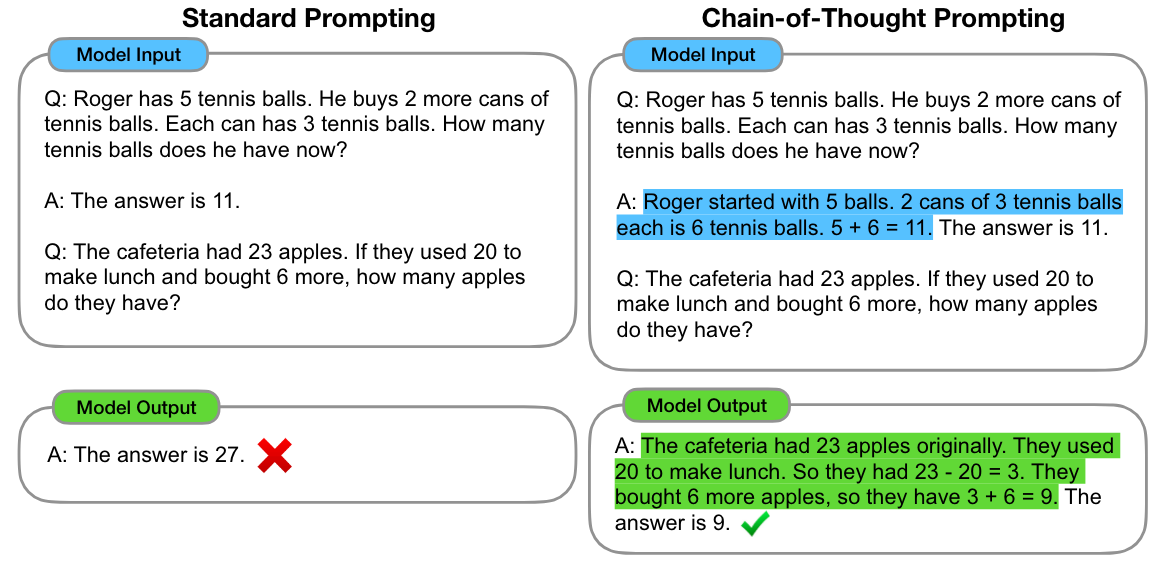
\includegraphics[width=0.8\linewidth]{pict/01/cot.png}
   \caption[Chain-of-Thought プロンプティングの例]{Chain-of-Thought プロンプティングの例 \protect\footnotemark}
   \label{cot}
\end{figure}
\footnotetext{\cite{wei23}より引用}

そこで我々は, 直感的な操作により LLM とのインタラクティブなストーリー共創手法を提供するクリエーターと LLM との仲介システムを web アプリケーションとして開発した. 本システムは, 物語構造分析を活用したLLMの制御を容易な操作により実現するインターフェースと, 繰り返し LLM を作用させることで創造性を高める体系的な創作プロセスを提供する. これらの機能を通じて本システムはストーリークリエーターとLLMとの仲介を担う御用聞きとして機能する.

本研究では, 開発したシステムを「TEZUKA2023プロジェクト\footnotemark \footnotetext{\url{https://tezukaosamu.net/jp/mushi/entry/26751.html} (cited 2024-01-27)}」において手塚治虫の漫画『ブラック・ジャック』\cite{Tezuka77}の新作エピソードの制作に活用してもらい, この取り組みを通じてアンケートの実施と操作ログの取得を行い本システムの有用性について考察した.

なお, 筆者自身の取り組みは以下の通り.
\begin{itemize}
   \item プロンプトの叩き台の提案
   \item プロンプト内における物語構造分析の展開要素の入れ込み方の提案
   \item タイトルおよびあらすじを生成させることの提案
   \item フリーワードによる編集機能の提案
   \item プロット編集セクションにおける一部機能の実装
   \item シナリオ生成セクションにおける一部機能の実装
   \item シナリオ編集セクションにおける一部機能の実装
   \item アンケートの作成
   \item アンケートの分析
   \item 操作ログの分析
\end{itemize}

これらの取り組みについて, プロンプトの叩き台の提案, プロンプト内における物語構造分析の展開要素の入れ込み方の提案については\ref{sec:prompt}節で述べ, タイトルおよびあらすじを生成させることの提案については\ref{self_method}項で, その結果と考察については\ref{self_result}節で, フリーワードによる編集機能の提案については\ref{subsec: freeword}項で, またその結果については\ref{subsec: edit_result}項で, プロット編集セクション等機能の実装については\ref{sec:implementation}節で, アンケートの作成については\ref{quetionnaires}項で, アンケートの分析と操作ログの分析については \ref{quetionnaire_result}節および\ref{log}節で述べる.

本論文の構成は以下の通りである. 第\ref{chap:background}章では, 本研究において開発したシステムが依拠するところの大きい物語構造と大規模言語モデルについて述べ, 第\ref{chap:relatedworks}章では, 関連研究について紹介する. 第\ref{chap:proposedmethod}章では, LLMとのインタラクティブな共創手法を提供するストーリー創作支援システムの提案を行い, 第\ref{chap:experiment}章では, 本システムの有用性を認識するために行われた具体的活用事例について, その詳細と得られた結果および考察について述べる. 最後に第\ref{chap:conclusion}章で結論を述べる.

%そこで我々は, 物語構造を活用し, プロのストーリークリエーターが LLM を用いたストーリー創作を効率的に行うことができる, ユーザーと LLM の仲介を担う御用聞き AI を web アプリとして開発した. このアプリケーションは画面の指示に従う直感的な操作で, 物語構造分析に基づいたプロット生成を実現する. さらに, 生成されたプロットの改善を目的とする, LLM との体系的でインタラクティブな共創手法を提供する. 我々はこのアプリケーションの開発により, LLM を活用したプロのストーリークリエーターの創作支援を探求した.


% \section{本論文の構成}
% 第2章では，ボトムアップ型を取り巻く複雑系という概念を紹介し，階層構造がどのようなものであるかを述べる．
% 第3章では，身体を動的に形成し，身体機能や行動を変化させていく仮想生命体モデルについて紹介する．
% 第4章では，本研究で提案する仮想生命体モデルについて紹介し，構築したシミュレーション環境について述べる．
% 第5章では，シミュレーションの結果とその考察を述べる．
% 第6章では，第5章の内容を元に提案した仮想生命体モデルがどのようであったかについてまとめ，今後の課題について述べる．



\expandafter\ifx\csname ifdraft\endcsname\relax
   \fancyhead[LO]{}
   \printbibliography[title=参考文献]
   \end{document}
   \fancyhead[LO]{\rightmark}
\fi
\documentclass[a4j,12pt]{jsreport}
% 数式
\usepackage{amsmath,amsfonts}
\usepackage{bm}

% 画像
\usepackage[dvipdfmx]{graphicx}

% biblatex
\usepackage[style=numeric, sorting=none, maxbibnames=1000]{biblatex}
\addbibresource{graduation_thesis.bib}

%itembox
\usepackage{ascmac}
%breakitemboxのためのpackage
\usepackage{itembkbx}
% \usepackage{tcolorbox} 画像が見えなくなってしまう原因
% \usepackage{framed} 枠

%フォント
\usepackage[ipaex]{pxchfon}

\usepackage[top=35truemm,bottom=30truemm,left=30truemm,right=30truemm]{geometry}
\usepackage{float}
\usepackage{multicol}
\usepackage{multirow}
\usepackage{paralist}
\usepackage{caption}
\usepackage{setspace}
\usepackage{algorithm}
\usepackage{algpseudocode}
\usepackage[dvipdfmx,hidelinks]{hyperref}
\usepackage{pxjahyper}
\usepackage{fancyhdr}
\usepackage{ltablex}
\usepackage{capt-of}
\usepackage{tabularx}
\usepackage{enumitem} % itemizeの行間 これは下になければならない
\usepackage{threeparttable} % 表の脚注
\usepackage{titlesec}
\titleformat{\chapter}[hang]{\LARGE\bfseries}{{\Large \prechaptername\thechapter\postchaptername}}{1em}{}


   \setlength{\headheight}{16.5pt}
   \captionsetup{format=hang}
\begin{document}
% ▼▼▼ 仕掛け：main じゃないとき（単体のとき）だけヘッダー設定 ▼▼▼
\ifdefined\ismain\else
   \pagestyle{fancy}
   \lhead{\rightmark}
   \renewcommand{\chaptermark}[1]{\markboth{第\ \thechapter\ 章\ #1}{}}
   \setlength{\headheight}{16.5pt}
   \titleformat{\chapter}[hang]{\LARGE\bfseries}{\prechaptername\thechapter\postchaptername}{1em}{}
\fi
% ▲▲▲▲▲▲▲▲▲▲▲▲▲▲▲▲▲▲▲▲▲▲▲▲▲▲▲▲▲▲▲▲▲▲▲▲

\chapter{関連研究}\label{chap:relatedworks}
本章ではまず, \ref{sec:language_model}節で本研究同様, アプリケーションとしてストーリー創作支援システムを構築し, その実践的な活用において有用性と課題が示された研究について紹介し, 次に\ref{sec:story_generation}節で, 物語の生成それ自体を目的とした研究について紹介する.

\section{言語モデルを活用した創作支援システム}\label{sec:language_model}


\section{物語生成}\label{sec:story_generation}
\subsection{Manga109Dataset}\label{sec:manga109}
本研究では，漫画画像に対応する脚本生成の基盤データとして，Manga109Dataset~\cite{matsui2017sketch,aizawa_building_2020} を採用した，Manga109は，1970年代から2010年代に出版された日本の商業漫画109作品（計 21,142 ページ）から構成され，数多くの研究で取り上げられてきた\cite{}学術利用可能な漫画画像データセットである．少年漫画，少女漫画，青年漫画など多岐にわたるジャンルと画風を網羅しており，特定の作家やスタイルに過学習することなく，汎用的な漫画の構造を学習する上で最適なデータセットといえる．本研究では，Manga109に含まれる全作品を対象とし，見開き画像を片側単ページに分割した上で，表紙や広告などを除く計19,555ページに対して脚本データの構築を行った．Manga109Dataset内に含まれる画像の一例を図~\ref{fig:manga109example}に示す．




\begin{figure}[htbp]
   \centering
   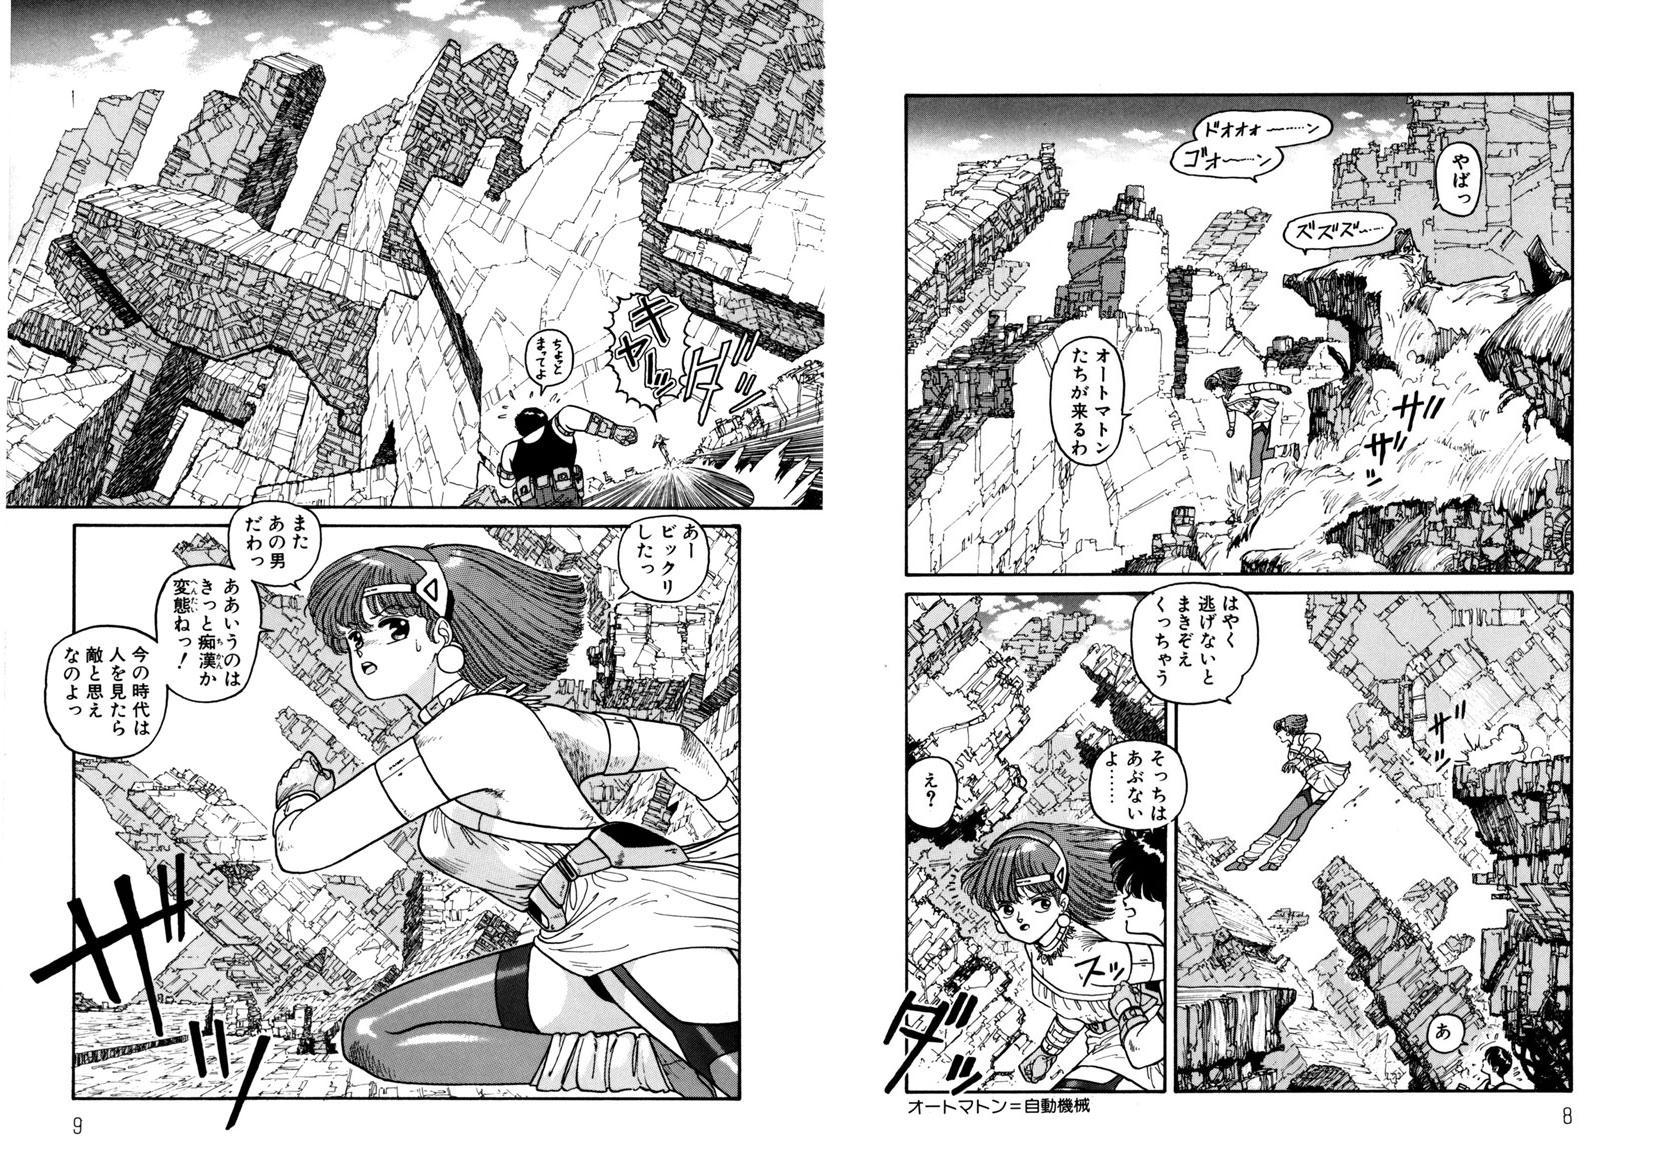
\includegraphics[width=0.9\linewidth]{pict/02/ARMS003.jpg}
   \caption{Manga109Dataset に含まれる漫画画像の例（『ARMS』より）．© 加藤 雅基／東京三世社}
   \label{fig:manga109example}
\end{figure}

% ▼▼▼ 仕掛け：main じゃないとき（単体のとき）だけ参考文献を表示 ▼▼▼
\ifdefined\ismain\else
   \printbibliography[title=参考文献]
\fi
% ▲▲▲▲▲▲▲▲▲▲▲▲▲▲▲▲▲▲▲▲▲▲▲▲▲▲▲▲▲▲▲▲▲▲▲▲

\end{document}
\expandafter\ifx\csname ifdraft\endcsname\relax
   \documentclass[a4j,12pt]{jsreport}
% 数式
\usepackage{amsmath,amsfonts}
\usepackage{bm}

% 画像
\usepackage[dvipdfmx]{graphicx}

% biblatex
\usepackage[style=numeric, sorting=none, maxbibnames=1000]{biblatex}
\addbibresource{graduation_thesis.bib}

%itembox
\usepackage{ascmac}
%breakitemboxのためのpackage
\usepackage{itembkbx}
% \usepackage{tcolorbox} 画像が見えなくなってしまう原因
% \usepackage{framed} 枠

%フォント
\usepackage[ipaex]{pxchfon}

\usepackage[top=35truemm,bottom=30truemm,left=30truemm,right=30truemm]{geometry}
\usepackage{float}
\usepackage{multicol}
\usepackage{paralist}
\usepackage{caption}
%\captionsetup{format=plain, justification=centering}
\usepackage{setspace}
\usepackage{algorithm}
\usepackage{algpseudocode}
\usepackage[dvipdfmx,hidelinks]{hyperref}
\usepackage{pxjahyper}
\usepackage{fancyhdr}
\usepackage{ltablex}
\usepackage{capt-of}
\usepackage{tabularx}
\usepackage{enumitem} % itemizeの行間 これは下になければならない
\usepackage{threeparttable} % 表の脚注
\usepackage{booktabs}
\usepackage{titlesec}
\titleformat{\chapter}[hang]{\LARGE\bfseries}{\prechaptername\thechapter\postchaptername}{1em}{}


   \setlength{\headheight}{16.5pt}
   \captionsetup{format=hang}
\begin{document}
% 上部のヘッダー
\pagestyle{fancy}
\lhead{\rightmark}
\renewcommand{\chaptermark}[1]{\markboth{第\ \thechapter\ 章\ #1}{}}
\fi

\chapter{Manga109ScriptDataset}\label{chap:proposedmethod}
本章では，本研究の第一段階において構築した，漫画画像に紐づく脚本データセットManga109ScriptDatasetについて，その構築手法や統計量，評価アノテーション手法の詳細を述べる．

序論で定義したとおり，本研究では漫画の「ネーム」を，幾何学的な「要素配置（Layout）」と「演出情報（Directions）」を統合した，物語と作品とを接続する中間表現として位置づける．このネーム生成に向けた取り組みに先立ち，第一段階では，物語としての「脚本」と「要素配置」との対応関係の学習に焦点を当て，Manga109ScriptDatasetを構築した．

構築においては，漫画画像を OpenAI API を介して GPT-4o に入力し，描画内容を脚本として記述させる手法を基本方針とした．本章では，この生成プロセスにおいて，モデルが複雑な文脈を正確に理解するために導入した画像加工やチャットフローの活用といった具体的な技術詳細について詳述する．

本章の構成は以下の通りである．まず~\ref{sec:dataset_design}節では，本データセットの基本設計として，対象データの概要および脚本形式の定義について述べる．続く~\ref{sec:visual_prompting}節では，LVLMのキャラクター認識精度の向上と，これに伴う正確な脚本生成を可能にするため実装したVisual Promptingについて述べる．\ref{sec:chat_flow}節では，画像間にまたがる連続的な文脈情報の理解を促進し，脚本内における物語の一貫性を確保することを目的に設計した，LVLMとのチャットフローについて示す．\ref{sec:statistics}節では，構築したデータセットの統計量を示し，最後に~\ref{sec:evaluation_data}節では，人手によるアノテーションに基づく脚本の品質評価手法と，その結果について論じる．

\section{本データセットの基本設計}\label{sec:dataset_design} 本節では，Manga109ScriptDatasetの構築において基盤となるManga109Datasetの選定理由および構築の対象とした記述フォーマットである脚本形式について述べる．

\subsection{Manga109Dataset}\label{sec:manga109} 　本研究では，漫画画像に対応する脚本生成の基盤データとして，Manga109Dataset~\cite{matsui2017sketch,aizawa_building_2020} を採用した，Manga109は，1970年代から2010年代に出版された日本の商業漫画109作品（計 21,142 ページ）から構成され，数多くの研究で取り上げられてきた\cite{}学術利用可能な漫画画像データセットである．少年漫画，少女漫画，青年漫画など多岐にわたるジャンルと画風を網羅しており，特定の作家やスタイルに過学習することなく，汎用的な漫画の構造を学習する上で最適なデータセットといえる．本研究では，Manga109に含まれる全作品を対象とし，見開き画像を片側単ページに分割した上で，表紙や広告などを除く計19,555ページに対して脚本データの構築を行った．Manga109Dataset内に含まれる画像の一例を図~\ref{fig:manga109example}に示す．

\begin{figure}[htbp]
   \centering
   \includegraphics[width=0.9\linewidth]{}
   \caption{Manga109Dataset に含まれる漫画画像の例}
   \label{fig:manga109example}
\end{figure}

\subsection{脚本形式} 　本研究において構築の対象とした物語文の形式は，日本の脚本形式に準拠する．脚本は映像制作現場において標準的に用いられる記述様式であり，テキストから視覚的イメージを具体化することを主目的として設計されている．その視覚化のための物語文というフォーマットは，ネーム生成というタスクにおいて親和性が高い．本研究では，Manga109が日本の漫画作品群であることを踏まえ，日本国内の制作様式において標準的に用いられている脚本形式をそのまま採用した．これは，将来的な制作支援応用を見据えた際，プロの作家や編集者が違和感なく扱える形式となるよう実応用性を考慮したためである，その形式は，以下の3つの主要な構成要素から成る．

\begin{enumerate}

   \item \textbf{柱}: 物語の場面転換を示すヘッダー情報．行頭に記号「◯」を付記し，その後に「場所」や「時間帯」を記述する（例：◯ 公園・昼）．

   \item \textbf{ト書き}:
         キャラクターの動作，表情，視線，および周囲の環境音や状況説明を記述する文章．視認性を高めるため，全角3文字分のインデント（字下げ）を行って記述する．これは，コマ割りや構図（カメラワーク）を示唆する重要な情報源となる．

   \item \textbf{セリフ}:
         キャラクターの発話内容．「話者名『セリフ内容』」の形式で記述する．
\end{enumerate}

本データセットの構築においては，漫画画像を入力とし，これらの構造化された物語文の構築を目指した．実際に生成された脚本の例を図~\ref{fig:script_example}に示す．

\section{Visual Prompting}\label{sec:visual_prompting}
本節では，LVLM の画像認識能力を補助し，正確な脚本生成を実現するために導入したVisual Prompting について述べる．

Manga109ScriptDataset の構築において，最も重要な要件の一つは，生成される脚本内で動作主や話者を正確に特定することである．しかし，第2章で述べた通り，漫画画像は白黒の線画表現であり、しばしばキャラクターが著しくデフォルメされるといった独自のドメイン特性を持つため，GPT-4o などの最新 LVLM であっても，そのまま適用するだけでは正確な認識，特にキャラクターの識別は十分になされない\cite{}．そこで本研究では，登場人物を取り違え，物語の整合性を著しく損なうハルシネーションを抑制するための手段として，画像内に視覚的な手がかりを直接埋め込む Visual Prompting を採用した．キャラクターの顔を色のついた円で囲い，視覚的な識別補助を与える手法である．

Manga109Dataset には，キャラクターの顔領域を示す Bounding Box が付与されており，各領域は作品内で一意のキャラクターIDと紐付いている．本研究ではこの情報を利用し，以下の手順で画像に加工を施した．まず，作品内に登場するキャラクターIDごとに，HSV色空間上で等間隔となるよう識別性の高い色を動的に割り当てる．次に，各顔領域に対して，割り当てた色で顔を囲う円を描画した．図\ref{fig:visual_prompting_example}に加工後の画像を示す．

\begin{figure}[htbp]
   \centering
   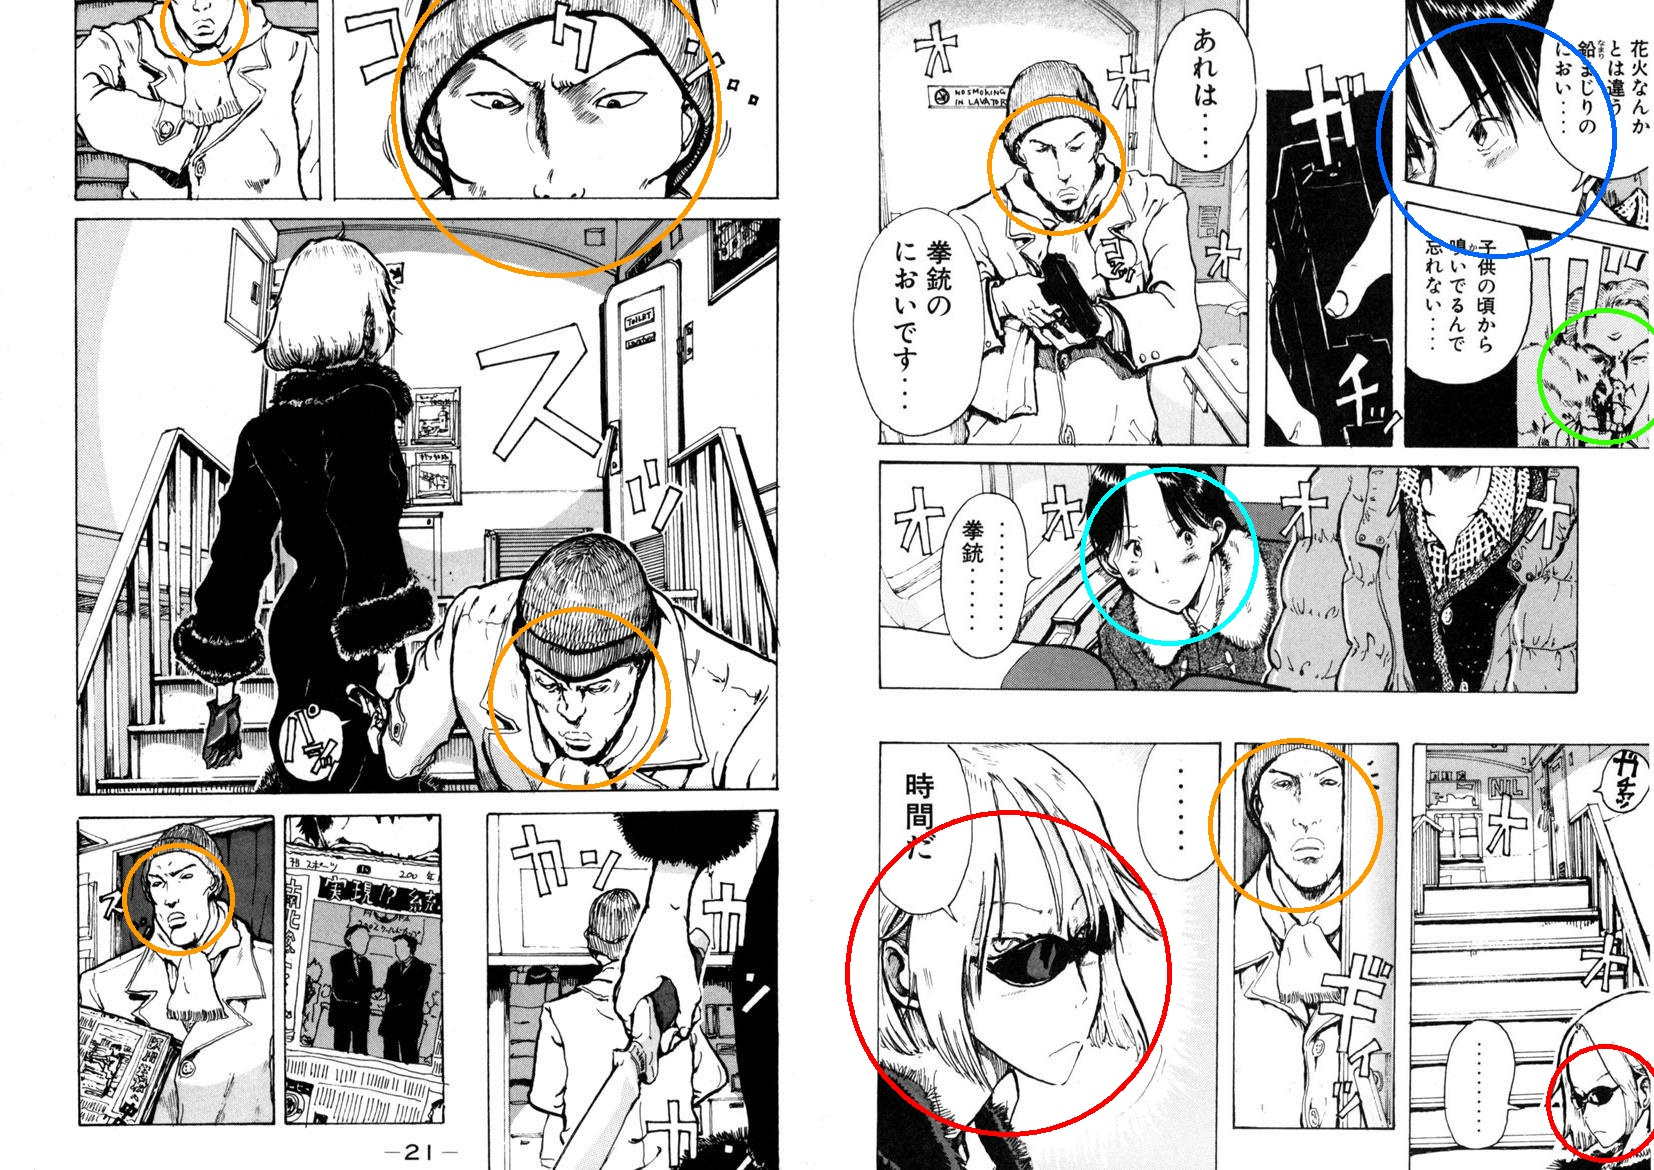
\includegraphics[width=0.9\linewidth]{pict/03/HanzeiKousyouninMinegishiEitarou10.jpg}
   \caption{Visual Prompting の例}
   \label{fig:visual_prompting_example}
\end{figure}

このアプローチは，Shtedritskiら~\cite{shtedritski_what_2023} の手法を漫画ドメイン向けに適応させたものである．この処理により，LVLM はデフォルメされた顔の識別といった高難度なタスクを色の識別という単純な視覚タスクへ置き換えることが可能となる．結果として，複雑な線画や類似したキャラクターが混在するシーンにおいても，モデルは視覚的アンカーを手がかりとして強固にキャラクターの識別能力を向上させた．

\section{画像間文脈理解のためのチャットフロー}\label{sec:chat_flow}
本節では，ページ間の文脈を考慮し，物語の一貫性を担保するために設計したチャットフローについて述べる．

\subsection{入力データの前処理と順序決定}
前節で述べた Visual Prompting に加え，モデルがキャラクターの同一性や会話の文脈を正しく理解するためには，正確なテキスト情報とその読み順が不可欠である．そこで本研究では，以下の2つの外部情報を利用し，漫画画像内の一連のセリフをプロンプト内で提示した．

\begin{enumerate}
   \item \textbf{テキストアノテーション}:
         各フキダシ内のテキスト内容および話者名については，Manga109Dialog~\cite{li_manga109dialog_2024} のアノテーションデータを使用．

   \item \textbf{読み順の決定（Magiアルゴリズム）}:
         コマやフキダシの読み順決定には，Sachdevaら~\cite{sachdeva_manga_2024} による Magi アルゴリズムを採用．
\end{enumerate}

ここで Magi を採用した理由は，LVLM 単体での空間的な順序推定能力の限界にある．我々の予備実験において，GPT-4oに画像のみを与えて読み順を推定させたところ，サンプリングした109ページ中，正解したのはわずか26ページに留まった．対照的に，ルールベースの手法である Magi を用いた場合，96ページにおいて正確な順序が得られた．この結果は，脚本生成の前段階として，アルゴリズムによる明示的な順序決定が不可欠であることを示している．

\subsection{文脈維持のための3段階インタラクション}
複数ページにわたる連続した物語を矛盾なく記述するため，本研究では GPT-4o に対して単純な1往復の指示を与えるのではなく，各ページ $i$ の生成において以下の3つのコンポーネント（$\alpha, \beta, \gamma$）から成る構造化されたインタラクションプロセスを構築した．

\begin{itemize}
   \item \textbf{$\alpha(i)$: 大域的文脈の理解 } \\
         ここでは，ページ単位の処理に入る前に，脚本生成の対象となるページ$i$が含まれるエピソード全体の一連のセリフをモデルに入力する．モデルからの応答を「完了」の肯定的応答としてシミュレートすることで，チャット内における文脈理解状態を確立させた．

   \item \textbf{$\beta(i)$: ページ $i$ の脚本生成 } \\
         実際に脚本を生成するフェーズである．入力として，「Visual Prompting を施したページ $i$ の画像」，「ページ $i$ のセリフテキスト」，および「直前のステップ $\gamma(i-1)$ で生成された物語の要約（Summary）」を与える．
         ここで過去の要約を与えることにより，モデルは「前ページまでの展開」を踏まえた上で，整合性の取れたト書きやセリフを脚本形式で生成することが可能となる．

   \item \textbf{$\gamma(i)$: 文脈情報の要約と更新 } \\
         次ページ $i+1$ の生成に備え，ここまでの物語の展開を要約させるフェーズである．生成された脚本と対話履歴に基づき，ストーリーの現状（誰がどこで何をしているか）を要約として出力させ，これを次のステップ $\beta(i+1)$ の入力として再利用する．
\end{itemize}

\subsection{シーケンスの実行}
本研究では，各ページ $i$ の脚本生成において，物語の一貫性を保持するために以下のシーケンスを実行した．ここで，矢印は同一チャットセッション内での対話の遷移を示している．

\begin{itemize}
   \item \textbf{先頭ページ ($i=1$) の場合} \\
         過去の文脈が存在しないため，以下の順序で実行する．
         \[
            \alpha(1) \rightarrow \beta(1)
         \]
   \item \textbf{第2ページ以降 ($i \ge 2$) の場合} \\
         直前のページの生成結果を履歴として保持しつつ，以下の順序で実行する．
         \[
            \alpha(i) \rightarrow \beta(i-1) \rightarrow \beta(i)
         \]
\end{itemize}
このように，脚本生成 $\beta(i \ge 2)$ においては常に一つ前のやり取りを履歴に残し，物語の一貫性を保持する工夫とした．また，次ページへの文脈受け渡し用として要約を生成する際は，以下のシーケンスへと拡張した．
\begin{itemize}
   \item \textbf{先頭ページ ($i=1$) の場合}
         \[
            \alpha(1) \rightarrow \beta(1) \rightarrow \gamma(1)
         \]
   \item \textbf{第2ページ以降 ($i \ge 2$) の場合}
         \[
            \alpha(i) \rightarrow \beta(i-1) \rightarrow \beta(i) \rightarrow \gamma(i)
         \]
\end{itemize}

各作品に対し，この一連のインタラクションを最終ページまで反復的に適用することで，Manga109ScriptDataset の全データを構築した．

\section{データセットの統計量}\label{sec:statistics} 　構築された Manga109ScriptDataset の詳細な統計量を表~\ref{tab:statistics} に示す． 　チャットフローを用いた生成の結果，109作品・計19,555ページに対し，約2万7千件の柱，約14万件のト書き，および約13万件のセリフを含む脚本データが構築された．

\begin{table}[htbp]
   \centering
   \setlength{\abovecaptionskip}{2pt}
   \caption{ Manga109ScriptDataset の統計量．「Distinct character types」はページごとのキャラクターIDのユニーク数，「Distinct speaker types」はページごとの話者IDのユニーク数を示す． }
   \label{tab:statistics}
   \begin{threeparttable}
      {\setlength{\tabcolsep}{5pt}
         \begin{tabular}{l r r}
            \toprule
            \textbf{要素}             & \textbf{総数}   & \textbf{平均 (/頁)} \\ \midrule
            \multicolumn{3}{l}{\textit{レイアウト要素 }}                      \\
            \hspace{0.5em}総ページ数     & 19{,}555      & \textemdash      \\
            \hspace{0.5em}コマ数       & 103{,}850     & 5.31             \\
            \hspace{0.5em}キャラクター検出数 & 157{,}865     & 8.70             \\
            \hspace{0.5em}キャラクター種類数 & 60{,}812      & 3.11             \\
            \hspace{0.5em}フキダシ数     & 146{,}549     & 7.49             \\
            \hspace{0.5em}話者種類数     & 55{,}778      & 2.85             \\ \midrule
            \multicolumn{3}{l}{\textit{脚本要素 }}                         \\
            \hspace{0.5em}柱         & 26{,}931      & 1.38             \\
            \hspace{0.5em}ト書き       & 138{,}890     & 7.04             \\
            \hspace{0.5em}セリフ       & 134{,}901     & 7.10             \\
            \hspace{0.5em}総文字数      & 6{,}703{,}063 & 342.78           \\ \bottomrule
         \end{tabular}}
   \end{threeparttable}
   \vspace{-1.2em}
\end{table}

\section{品質評価}\label{sec:evaluation_data} 　構築されたデータセットの品質を検証するため，人手による評価実験を行った．

\subsection{評価手法と指標} 　一般的な画像キャプションの生成タスクとは異なり，本研究で生成する脚本には正解データが存在しない．また，脚本形式は単純な画像の言語化ではなく，前後の文脈的な整合性やより複雑な状況の記述が求められるため，BLEU~\cite{}やCIDEr~\cite{}といった既存の自動評価指標の適用は困難である．そこで本研究では，以下の5つの指標を定義し，人手による確認を行うことで品質を定量的に検証した．

\begin{enumerate} \item \textbf{柱の再現率}: 漫画画像内で描かれている場所やシーンが，生成された脚本の「柱」として正しく抽出されているか．

   \item \textbf{柱の適合率 }:
         生成された「柱」に記述されている場所が，実際に漫画画像内に描かれているか．

   \item \textbf{ト書きの適合率 }:
         生成された「ト書き」の内容が，対象ページの描画内容と合致しているか．ランダムに抽出された他ページのト書きと混ぜた状態で，正しく対象ページのものと判定できるかを確認．

   \item \textbf{文脈外ト書きの検出精度 }:
         他ページから混入させた無関係なト書きを，対象ページのものではないと正しく棄却できるか．

   \item \textbf{セリフの再現率}:
         漫画内のフキダシにあるセリフが，脚本内に漏れなく転記されているか．
\end{enumerate}

\subsection{実験設定と結果} 　評価データとして，Manga109Dataset の各作品から物語の連続性を保った状態で連続する約10ページをランダムに抽出し，合計1,000ページを評価対象とした．この1,000ページを500ページごとの2セットに分割し，計6名の評価者が分担して確認を行った（各ページにつき3名が重複して評価を実施）．なお，評価者には適切な報酬が支払われている．

評価の結果，各指標の平均スコアは以下の通りとなった． \begin{itemize} \item 柱の再現率: \textbf{0.793} \item 柱の適合率: \textbf{0.838} \item ト書きの適合率: \textbf{0.664} \item 文脈外ト書きの検出精度: \textbf{0.910} \item セリフの再現率: \textbf{0.988} \end{itemize}

セリフの再現率がほぼ1.0に近い値を示していることから，フキダシの内容は極めて正確に脚本化されていることがわかる．また，ト書きに関しても高い検出精度を示しており，生成されたデータセットが十分な信頼性を有していることが確認された．



\expandafter\ifx\csname ifdraft\endcsname\relax
\fancyhead[LO]{}
\printbibliography[title=参考文献]
\end{document}
\fancyhead[LO]{\rightmark}
\fi
\input{04_script2layout.tex}
\documentclass[a4j,12pt,dvipdfmx]{jsreport}

% 数式
\usepackage{amsmath,amsfonts}
\usepackage{bm}

% 画像
\usepackage[dvipdfmx,top=35truemm,bottom=30truemm,left=30truemm,right=30truemm]{geometry}
\usepackage[dvipdfmx]{graphicx}
% biblatex
\usepackage[style=numeric, sorting=none, maxbibnames=1000]{biblatex}
\addbibresource{graduation_thesis.bib}

% itembox
\usepackage{ascmac}
% breakitemboxのためのpackage
\usepackage{itembkbx}
% \usepackage{tcolorbox} 画像が見えなくなってしまう原因
% \usepackage{framed} 枠

% フォント
\usepackage[ipaex]{pxchfon}
\listfiles
\usepackage{float}
\usepackage{multicol}
\usepackage{multirow}
\usepackage{paralist}
\usepackage{caption}
% \captionsetup{format=plain, justification=centering}
\usepackage{setspace}
\usepackage{algorithm}
\usepackage{algpseudocode}
\usepackage[dvipdfmx,hidelinks]{hyperref}
\usepackage{pxjahyper}
\usepackage{fancyhdr}
\usepackage{ltablex}
\usepackage{capt-of}
\usepackage{tabularx}
\usepackage[export]{adjustbox}
\usepackage{booktabs}
\usepackage{enumitem} % itemizeの行間 これは下になければならない
\usepackage{threeparttable} % 表の脚注
\usepackage{titlesec}
\usepackage{makecell}
\usepackage{forest}
\usepackage{fancybox}
% titlesec と \paragraph の相性問題を回避（run-in 見出しにする）
\titleformat{\paragraph}[runin]
  {\normalfont\normalsize\bfseries}
  {}{0pt}{} % ←ここには文字や \noindent 等を入れない
\titlespacing*{\paragraph}
  {0pt}{1.0ex}{0.8em}
\titleformat{\chapter}[hang]{\LARGE\bfseries}{\prechaptername\thechapter\postchaptername}{1em}{}

\setlength{\headheight}{16.5pt}
\captionsetup{format=hang}
\captionsetup[figure]{font=small}
\captionsetup[table]{font=small}
\begin{document}

% ▼▼▼ 仕掛け：main じゃないとき（単体のとき）だけヘッダー設定 ▼▼▼
\ifdefined\ismain\else
   \pagestyle{fancy}
   \lhead{\rightmark}
   \renewcommand{\chaptermark}[1]{\markboth{第\ \thechapter\ 章\ #1}{}}
   \setlength{\headheight}{16.5pt}
   \titleformat{\chapter}[hang]{\LARGE\bfseries}{\prechaptername\thechapter\postchaptername}{1em}{}
\fi
% ▲▲▲▲▲▲▲▲▲▲▲▲▲▲▲▲▲▲▲▲▲▲▲▲▲▲▲▲▲▲▲▲▲▲▲▲

\chapter{Manga109NameDataset}\label{chap:manga109name}

本章では，本研究の第二段階として構築した，
漫画ネームデータセット Manga109NameDataset について述べる．
本データセットは，漫画画像に紐づく脚本情報に加え，
詳細な演出情報を体系的に付与したものであり
物語から漫画作品へと至る過程を，
より高次な構造として捉えることを目的としている．

前章では，
Manga109ScriptDataset を用いた
脚本に基づく漫画レイアウト生成手法を検討し，
脚本情報が要素配置の精度や
ページ全体の幾何的一貫性に寄与することを示した．
しかし，序論で述べたとおり，
漫画制作におけるネームは，
単なる要素の配置結果ではなく，
視線誘導や強調，感情表現といった
演出上の意思決定が統合された，
より複合的な中間表現である．
そのため，
レイアウト生成のみを対象とした前章の設定では，
ネームが本来担う表現的側面を
十分に扱うことはできない．
本来の漫画制作におけるネームは，
作画に先立つ下書きとして描かれる視覚的な表現であるが，
本研究では，このネームを画像そのものとして直接扱うのではなく，
その中に含まれる本質的な設計要素を抽出し，
要素の幾何学的配置を表すレイアウト情報と，
演出上の意図を言語的に記述した演出情報とに分解する．
そして，これらを統合した構造化表現としてネームを定義する．
この抽象化は，
ネームが担う配置設計および演出上の意思決定を保持しつつ，
脚本からネーム生成へ至る過程を
計算機上で段階的に扱うための，
本研究における操作的定義である．

以上を踏まえ，本研究では，
近年のLVLMの性能向上を背景として，
漫画画像から脚本情報を改めて抽出し直すとともに，
キャラクターの振る舞いや表情，カメラワークといった
演出情報を新たに獲得し，
これらを構造的に整理した
Manga109NameDataset を構築した．
本研究では，このデータセットを，
後続章で扱う脚本に基づくネーム生成モデルの
学習および評価に適した基盤データとして位置づける．

本章の構成は以下の通りである．
まず~\ref{sec:name_overview} 節において，取り扱う演出情報に触れながら，
Manga109NameDataset の概要とそのデータ構造を説明する．
続いて~\ref{sec:name_construction} 節において，
データセットの構築にあたって整備した
読み順アノテーションおよび
独自のVisual Prompting の詳細，データセット構築の実行手順を説明する．
次に~\ref{sec:name_statistics} 節で，
構築したデータセットの統計量を示し，最後に~\ref{sec:name_sample} 節で構築したデータの可視化例を示す．

\section{Manga109NameDataset の概要}\label{sec:name_overview}
図\ref{fig:narrative_graph}に，
Manga109NameDataset における1サンプル分のデータ構造の概略を示す．
\begin{figure}[htbp]
   \centering
   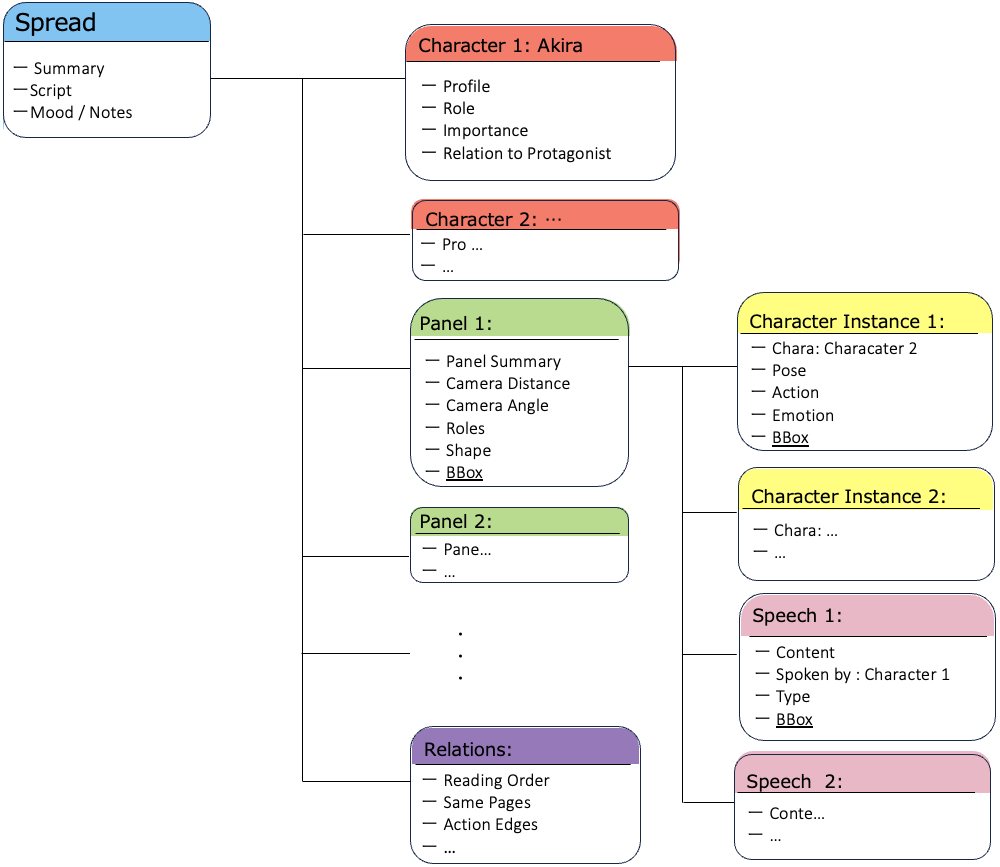
\includegraphics[width=\linewidth]{pict/05/narrative_graph.png}
   \caption{Manga109NameDataset における1サンプル分のデータ構造の概略}
   \label{fig:narrative_graph}
\end{figure}

Manga109NameDataset は，
漫画のネームを，
要素の幾何学的配置を表すレイアウト情報と，
脚本形式の記述を含む物語文章および演出情報を構造化したデータセットである．
本データセットでは，
漫画の見開きページ一つを基本単位とし，
その内部に含まれるコマ，キャラクター，セリフといった要素を
ノードとして定義するとともに，
それらの包含関係，参照関係，順序関係，および相互作用を
エッジとして明示的に表現する．
これにより，
ネームを構成要素と関係性の集合として捉え，
配置設計と演出上の意思決定を
計算機上で扱いやすい形式へと整理している．なお，見開き単位でデータを取得したのは，漫画の紙面構造上，見開きを一枚絵として捉え演出が設計されることが多いためである．

このように構成されたグラフにおいては，図\ref{fig:narrative_graph}に示すように
見開き全体に対応する \textbf{Spread ノード}を
物語および演出の文脈を担う最上位ノードとして位置づけている．
Spread ノードには，
当該場面の内容を要約した概要文や脚本記述，
場面全体の雰囲気や演出上の補足といった
グローバルな物語情報が付与される．
これらは，
配下に接続される各コマやキャラクター，セリフといった要素を，
個別の配置や表現としてではなく，
場面全体の流れや意図の中で解釈するための
上位文脈として機能する．

Spread ノードの下位には，
見開き内の各コマに対応する \textbf{Panel ノード}が配置される．
Panel ノードは，
漫画における最小の視覚的・演出的単位として，
物語の進行や演出上の役割を担う要素である．
各 Panel ノードには，
当該コマの内容を簡潔に記述した要約文に加え，
対話，反応，間（ま）といった物語上の役割，
コマ形状やカメラ距離・アングルといった
演出に関わる属性が付与される．
これにより，
コマ単体の意味内容と，
見開き全体における役割とを分離して記述することが可能となり，
レイアウト設計および演出制御の双方を
明示的に扱える構造となっている．

登場人物に関しては，
物語上の人物そのものを表す \textbf{Character ノード}と，
特定のコマ内に描かれた具体的な出現を表す
\textbf{Character Instance ノード}を分離して定義している．
Character ノードには，
人物名や性格，物語上の立ち位置といった
作品全体で共有される属性が付与される．
一方，
Character Instance ノードは，
特定のキャラクターの描写を表すノードであり，
姿勢，動作，感情といった
視覚的・演出的な具体像が記述される．
この分離により，
同一人物が複数のコマに異なる表情や振る舞いで登場する状況を，
構造的に自然な形で表現できる．

セリフは，
吹き出し単位で \textbf{Speech ノード}として管理される．
Speech ノードには，
発話内容のテキスト情報に加え，
発話の種類や，
どのキャラクター・どのコマに紐づくかといった
参照関係が付与される．
これにより，
言語表現と視覚要素との対応関係を
明示的に扱うことが可能となっている．

これらの各ノード間には，
包含関係，参照関係，順序関係，および相互作用を表す
複数種のエッジが定義されている．
これにより，
漫画ネームに内在する
空間的構造，時間的順序，および物語的関係性を，
単一のグラフ構造として統合的に表現している．また，直接的に紙面に描画される要素であるノード，Panel ノード，Character Instance ノード，Speech ノードには，バウンディングボックスの値を持たせ，レイアウト情報を表現している．

以上のように，Manga109NameDataset では，
見開き，コマ，キャラクター，セリフといった各要素を
グラフ上のノードとして整理し，
それぞれに対応する描画内容や場面における詳細な情報を集約することで，
漫画ネームに内在する演出上の意思決定を
構造化された形で表現している．
この構造により，
脚本に基づくネーム生成やレイアウト生成といった後続の処理において，
物語文脈，演出意図，および配置情報を
統合的に扱うことが可能となる．

\section{データセット構築手法}\label{sec:name_construction}
Manga109NameDataset の構築は，
Manga109ScriptDataset の構築と同様に，
LVLMを用いて漫画画像から必要な情報を抽出することを基本方針としている．
一方で，本データセットの構築では，
データの取得単位をページ単位ではなく見開き画像単位へと拡張し，
より高次な文脈および演出情報を扱う点で設定が異なる．
使用した LVLM は，
Gemini 3~\cite{woodward2025gemini3} および GPT-5.2~\cite{openai2025gpt52} であり，いずれも API を介して利用した．

漫画画像の読解における困難さについては，
Manga109ScriptDataset の構築過程において既に議論したとおりであり，
特に読み順の推定やキャラクターの識別は，
LVLM にとって依然として難しい課題である．
Manga109NameDataset の構築においても，
これらの問題は引き続き重要であり，
加えて見開き単位での処理に伴う
文脈の拡張や要素数の増加が新たな難点となる．

そこで本研究では，
ScriptDataset 構築時の知見を踏まえ，
読み順の明示的な付与や，
キャラクター識別を補助するための情報付加など，
複数の追加的工夫を導入することで，
これらの課題に対処した．
以下では，
Manga109NameDataset の構築に際して新たに導入した
各手法について順に説明する．

\subsection{読み順アノテーションの付与}\label{sec:reading_order_annotation}

漫画の内容理解において，
コマおよびセリフの読み順は，
物語構造を復元するための最も基本的な前提条件である．
Manga109ScriptDataset の構築においても，
読み順の推定が LVLM にとって困難であること，
既存手法による自動推定では誤りが残ることを確認している．
この問題は，
見開き単位で物語と演出を統合的に扱う
Manga109NameDataset においては，
より深刻な影響を及ぼす．

特に本データセットでは，
コマ間の時間的順序だけでなく，
セリフ間の発話順，
さらには演出上の「間（ま）」や反応の連なりを
正確に復元する必要がある．
そのため，
既存の自動推定結果や推論に依存するのではなく，
読み順を明示的な正解情報として与えることが不可欠であると判断した．

そこで本研究では，
Manga109Dataset に含まれる
全コマ 103{,}850 枚および
全セリフ 127{,}877 件に対して，
人手による読み順アノテーションを新たに付与した．
アノテーションは，
見開き内における読み進め順を基準として，
コマおよびセリフに一意な順序を割り当てる形で行った．

アノテーション作業にあたっては，
効率的かつ一貫した作業を行うため，
本研究独自のアノテーションツールを開発した．開発したツールを操作画面を図~\ref{fig:reading_order_tool} に示す．

\begin{figure}[htbp]
   \centering
   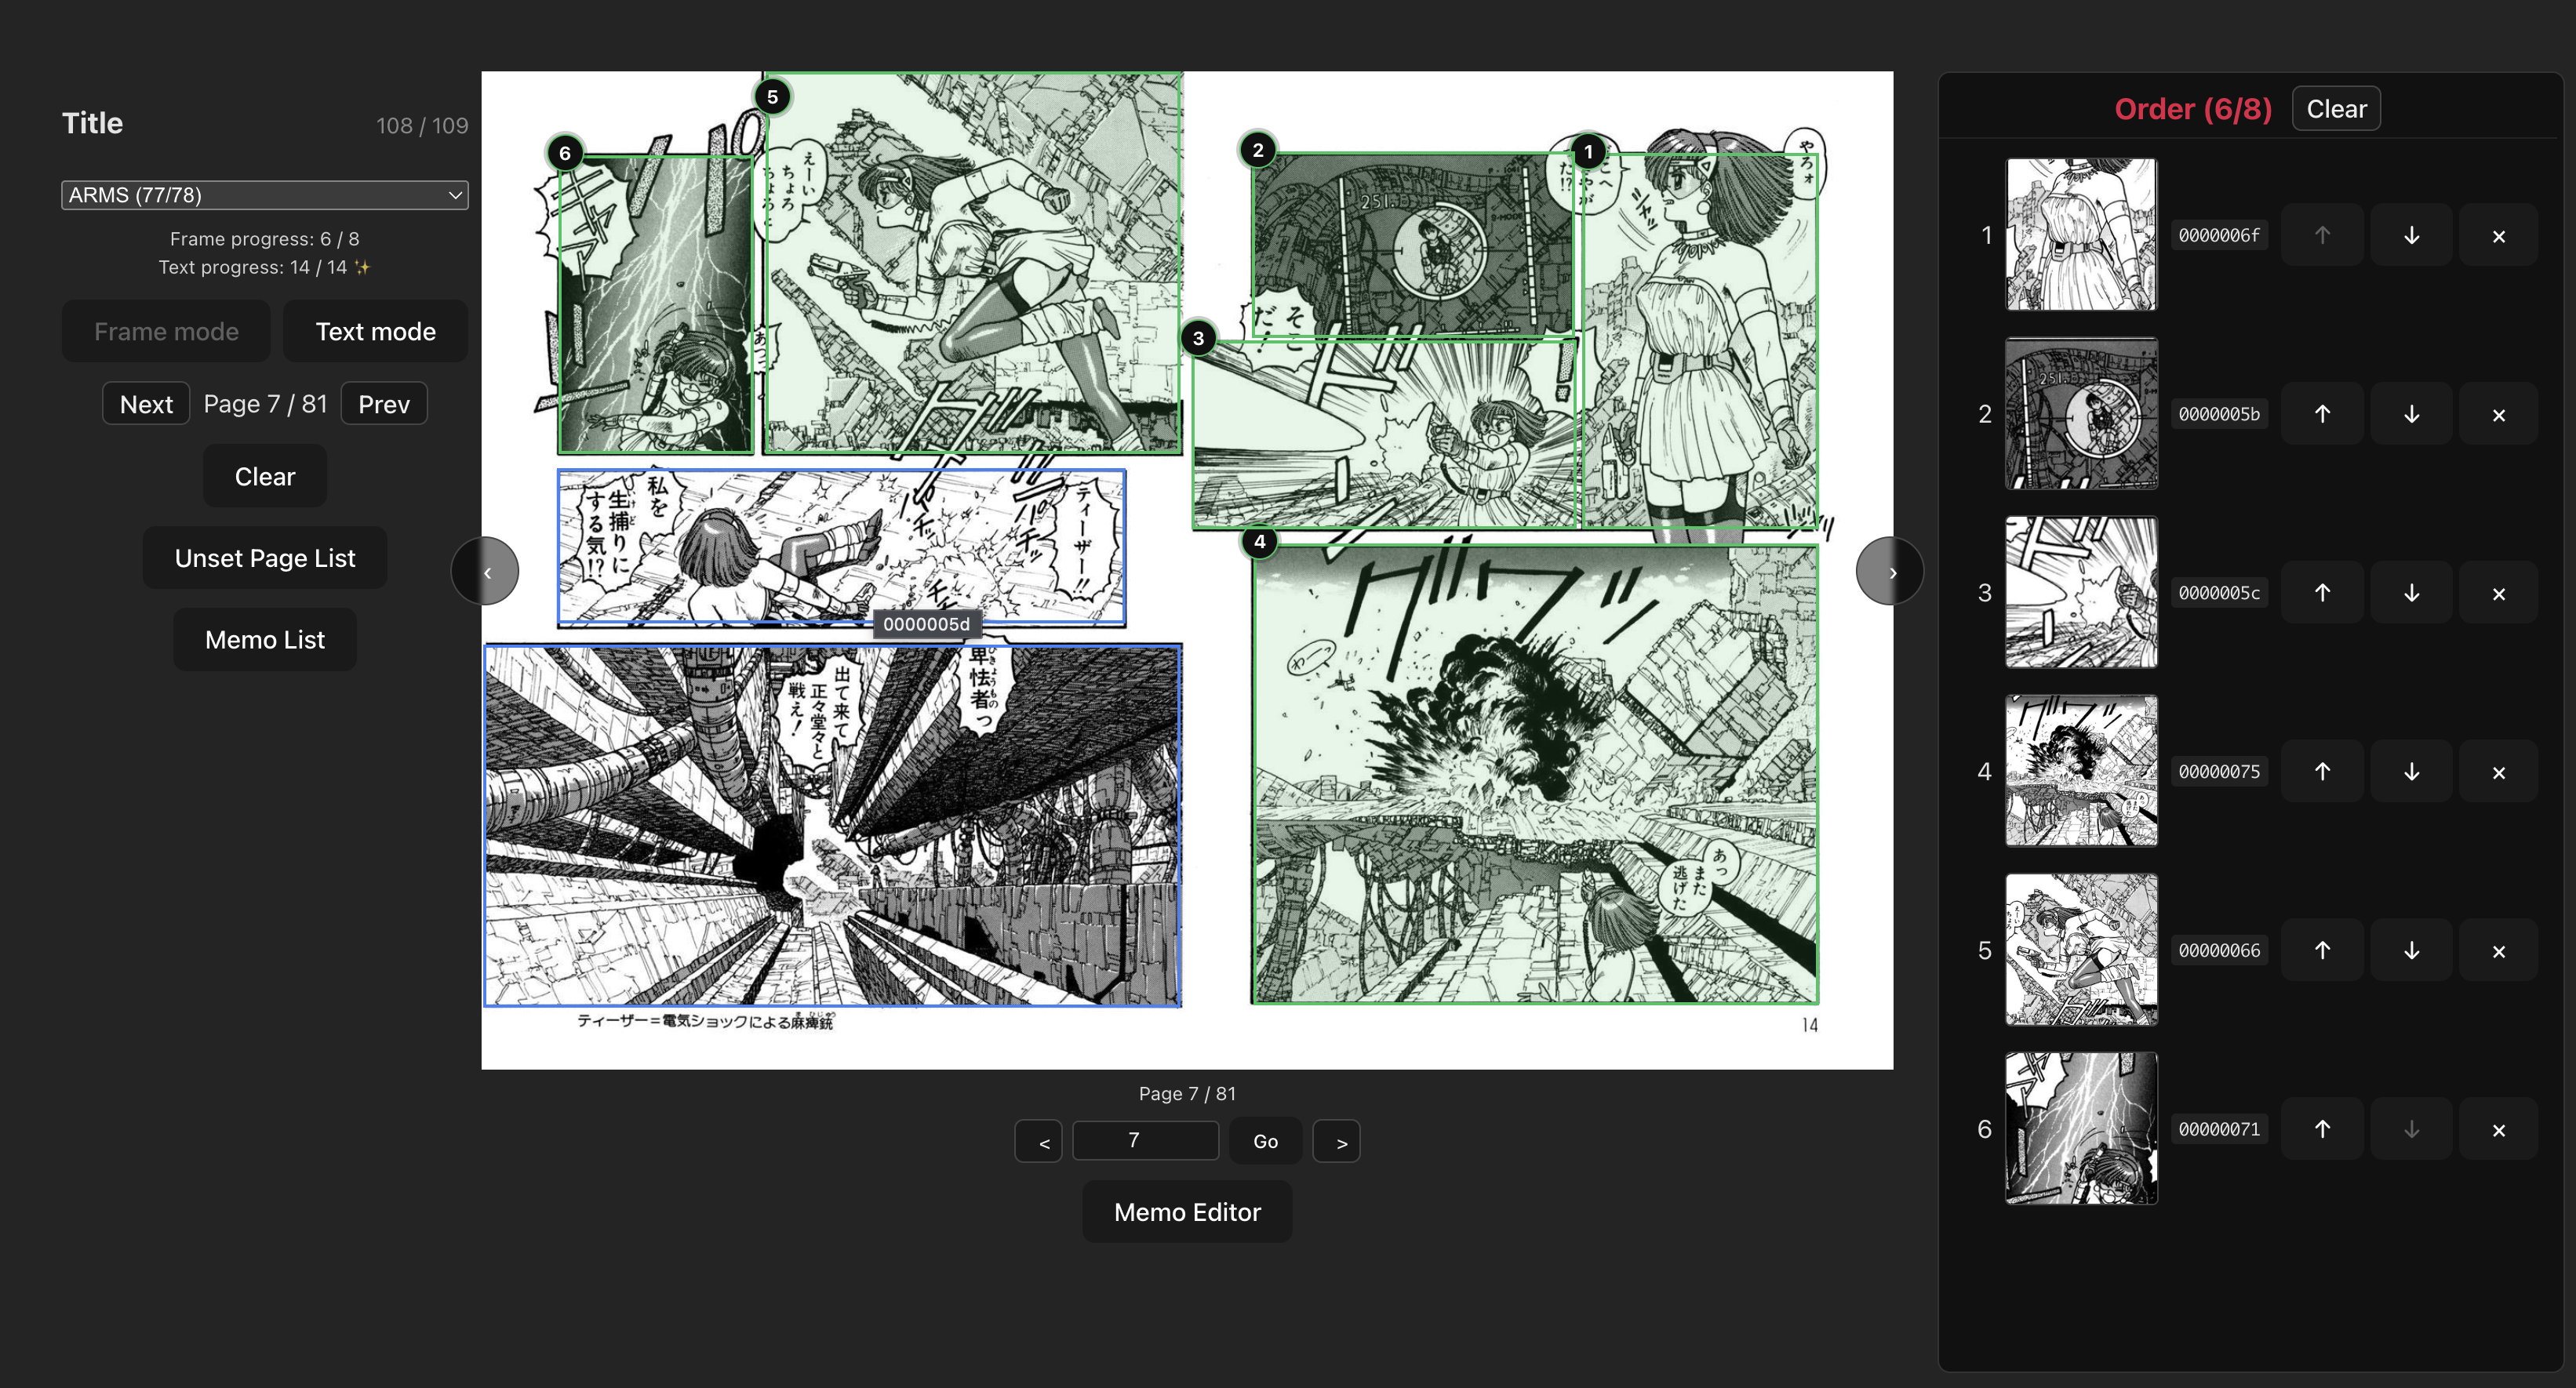
\includegraphics[width=\textwidth]{pict/05/reading_order_tool.png}
   \caption{読み順アノテーションツールの操作画面(漫画:『ARMS』©加藤 雅基/東京三世社)}
   \label{fig:reading_order_tool}
\end{figure}

本ツールでは，
見開き画像を表示しながら，
コマおよびセリフを選択し，
直感的に順序を指定できるインタフェースを備えている．
実作業は，
筆者が中心となって進めるとともに，
一部については産業技術総合研究所の技術支援者の協力を得て実施した．

このようにして付与された読み順アノテーションは，
後述するビジュアルプロンプティングにおいて
LVLM に与える重要な手がかりとして利用されるほか，
データセット全体の構造的整合性を保証する基盤情報として機能する．

\paragraph{既存手法との読み順の差異}
読み順推定手法として知られる Manga Whisperer~\cite{sachdeva_manga_2024-1}のアルゴリズムについて，
本研究では，
人手アノテーションとの順序一致率を比較評価した．
その結果，
見開き画像単位で順序が完全一致しなかった割合は，
コマについて 1{,}121 / 10{,}122（11.87\%），
セリフについて 2{,}609 / 10{,}043（25.98\%）であった．
本研究では，
コマ単位やセリフ単位での部分的な誤りの定義が困難であることから，
順序が完全一致しなかった見開き画像の割合を指標としている．

図~\ref{fig:reading_order_diff1}，~\ref{fig:reading_order_diff2} に，
それぞれコマとセリフの読み順が一致しなかった見開き画像の例を示す．


\begin{figure}[htbp]
   \centering
   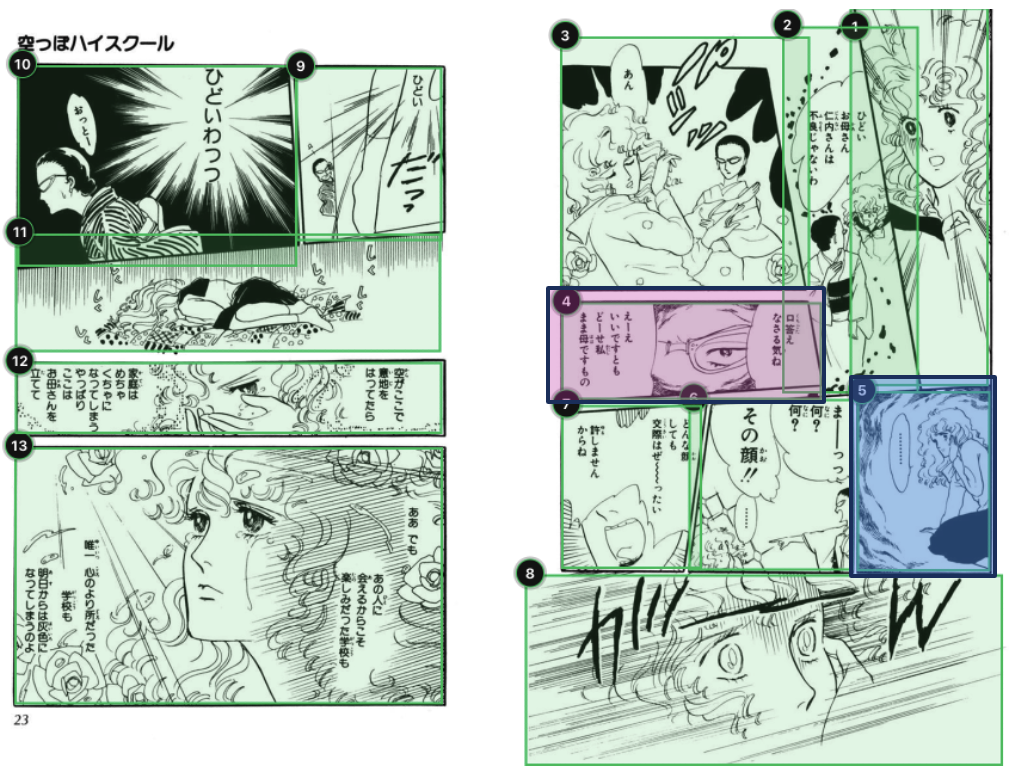
\includegraphics[width=\textwidth]{pict/05/reading_order_diff1.png}
   \caption{コマの読み順が一致しなかった見開き画像の例．本来は4，5と読み進めるべきコマの順序が，自動推定では逆転してしまった(漫画:『空っぽハイスクール』©	高口 里純/角川書店)．}\label{fig:reading_order_diff1}
\end{figure}

コマの読み順について，
Magi による自動推定が正しく行えなかった事例を分析した結果，
図~\ref{fig:reading_order_diff1} に示すように，
長方形近似に基づく配置推定の影響や，
左上と右下に配置されたコマ同士の比較において
内容理解を要する場合，
さらに吹き出しによる視線誘導が
コマの幾何学的配置による優先順位を凌駕する場合などが確認された．
これらの事例では，
単純な空間配置に基づく規則のみでは，
実際の読解順を適切に復元できないことが分かる．


\begin{figure}[htbp]
   \centering
   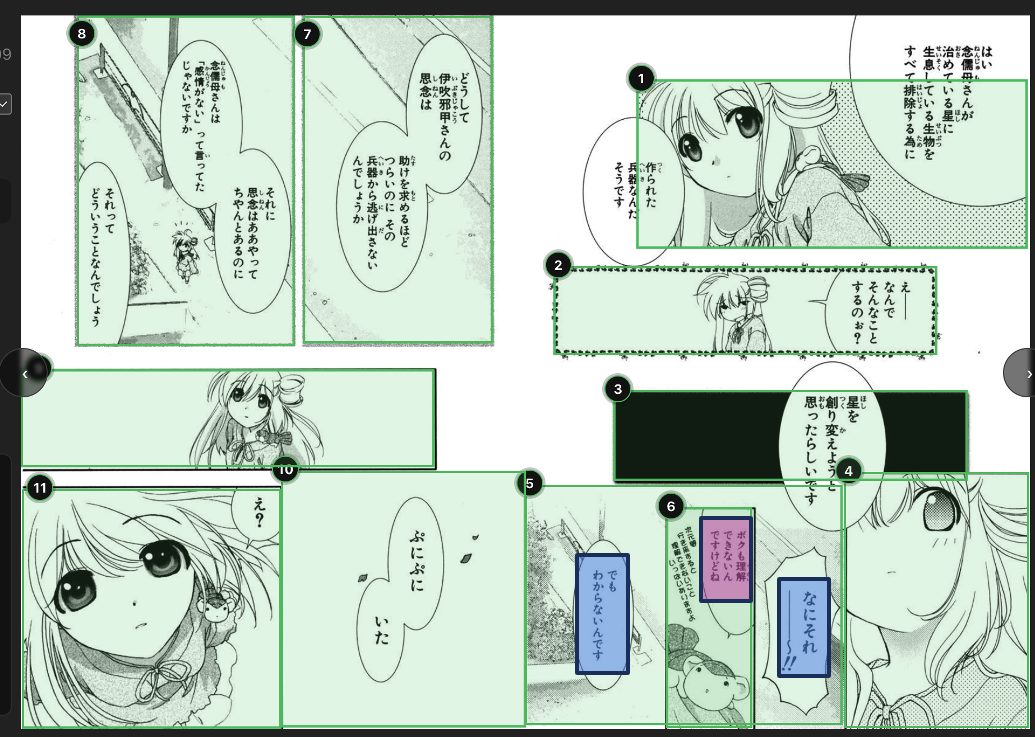
\includegraphics[width=\textwidth]{pict/05/reading_order_diff2.png}
   \caption{セリフの読み順が一致しなかった見開き画像の例．本来は6番のコマに帰属するセリフは，5番のコマに帰属する２つのセリフの間で読まれるべきであるが，自動推定では5番のコマの２つのセリフよりも後に推定されてしまった(漫画:『ヒーリング・プラネット』©桜野 みねね/	エニックス)．}\label{fig:reading_order_diff2}
\end{figure}

一方，セリフの読み順についても，
自動推定が困難となる特徴的な状況が観察された．
具体的には，図~\ref{fig:reading_order_diff2} に示したような
セリフの順序が帰属するコマの順序に強く制約される場合や，
本来的に明確な帰属先コマを持たない
「宙に浮いた」セリフが存在する場合である．
後者のようなケースでは，
アルゴリズム上，
最も近傍のコマに機械的に割り当てられることで
順序が決定されるため，
実際の読解順と乖離が生じやすい．
また，
左上と右下に配置されたセリフ同士の順序関係は
セリフ内容の意味理解に依存する場合も確認された．

以上の分析から，
漫画における読み順は，
コマ配置，吹き出しによる視線誘導，
内容理解，演出的意図といった
複数の要因が複合的に関与して決定されることが多く，
その自動推定は本質的に困難な課題であることが明らかとなった．
本研究では，
これらの問題に対処するため，
人手により付与した読み順アノテーションを
正解情報として利用し，
後続のデータ取得および LVLM による読解性能の基準として用いている．

\subsection{ID 情報を付記する独自 Visual Prompting}\label{sec:visual_prompting_with_id}

本研究では，
付与した読み順アノテーションを
LVLM による漫画理解および情報抽出に
効果的に反映させるため，
コマおよびセリフに一意な ID を付与し，
それを視覚的に画像上へ埋め込む
独自の Visual Prompting 手法を導入した．図~\ref{fig:visual_prompting_with_id}に実際に使用した Visual Prompting の例を示す．

\begin{figure}[htbp]
   \centering
   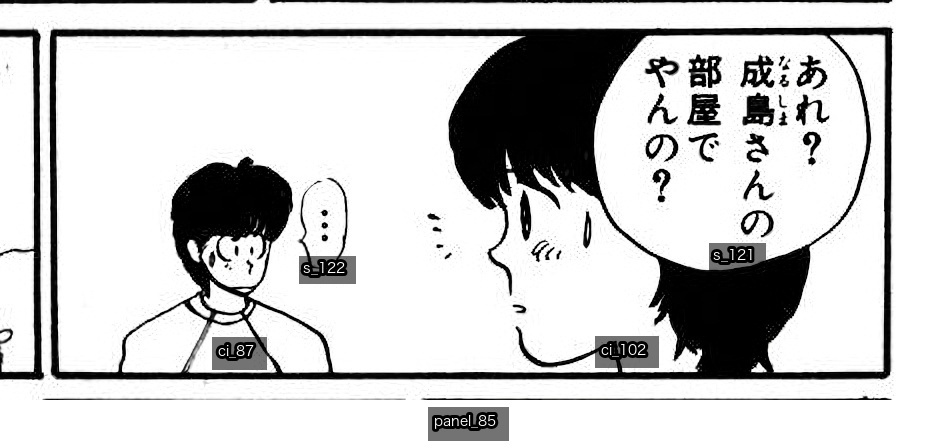
\includegraphics[width=\textwidth]{pict/05/id_visualprompting.jpg}
   \caption{IDを付記したVisual Prompting の例(漫画:『愛さずにはいられない』©よし まさこ/集英社)．}
   \label{fig:visual_prompting_with_id}
\end{figure}

Manga109ScriptDataset の構築においては，
ページ単位で漫画画像を入力し，
そのページ全体に対応する脚本を
一つのテキストとして生成すれば十分であった．
そのため，
生成された脚本と
画像内の個々のコマやセリフとの
厳密な対応関係を
明示的に管理する必要はなかった．

これに対し，
Manga109NameDataset では，
見開き内に含まれる
各コマ，各キャラクター，各セリフといった
描画要素ごとに，
演出情報や構造的な属性を
個別に抽出・整理することを目的としている．
すなわち，
本データセットの構築では，
「見開き全体から一つの脚本を得る」のではなく，
「見開き内の各描画要素から
それぞれに対応する情報を取得する」
という，より細粒度な対応付けが必要となる．

このような設定では，
LVLM が生成した記述と，
元画像上の具体的なコマやセリフ，
さらにはキャラクターの出現とを
正確に対応付けることが不可欠である．
しかし，
画像内に多数の要素が混在する漫画表現において，
自然言語による参照や
位置関係の暗黙的な推論のみに依存すると，
対応関係が曖昧になりやすい．

そこで本研究では，
読み順アノテーションに基づき，
各コマおよび各セリフに
連番の ID を付与するとともに，
これらの ID を
漫画画像上に直接描画した画像を
LVLM への入力として用いた．
具体的には，
見開き画像全体に加え，
各コマを個別に切り出した画像を
読み順に従って入力し，
それぞれの画像内に
対応するコマ ID やセリフ ID を
明示的に表示した．ID の表示は描画対象の画像領域に対する6\%の面積を占める小さな枠内に配置し，小さくなりすぎて認識されなくなることを防ぐため，最小フォントサイズを 12pt に設定した．

この ID 表示は，
単なるデータ管理上の識別子ではなく，
LVLM に対して
「どの要素を指しているのか」を
視覚的にアンカーする役割を果たす．
これにより，
生成される脚本記述や演出情報を，
特定のコマやセリフ，
さらにはキャラクターの具体的な出現と
一対一に対応付けることが可能となった．
また，
ID を介した参照により，
キャラクター名の誤同定や，
セリフと話者の取り違えといった
問題の発生を大きく抑制できることを確認している．

さらに，
画像入力の構成についても工夫を行った．
近年の LVLM においては
入力可能なトークン数が大幅に増加していることから，
本研究では，
対象とする見開き画像に加え，
当該見開き内の全コマを
個別画像として切り出し，
読み順に並べて入力する方式を採用した．
この際，
ID 表示は各コマ画像側に付与し，
見開き全体像と局所的な詳細情報とを
同時に参照できる構成とした．

このような
ID 情報を視覚的に付与する Visual Prompting により，
LVLM は，
漫画における空間配置と読み順，
物語的な対応関係，キャラクター識別を
より安定して理解できるようになり，
これはネーム構造の抽出精度向上に
大きく寄与した．

図~\ref{fig:panel_json_structure_with_id} に，付記した ID により，キャラクターの識別及び状況の理解が適切に行われた生成結果の例を示す．


\begin{figure}[htbp]
   \centering
   % 全体のレイアウト：左右に分割
   \begin{tabular}{@{}p{0.40\linewidth}@{\hspace{1em}}p{0.56\linewidth}@{}}
      % --- 左側：画像 ---
      % 画像内のID (s_12, ci_7など) が見えるように配置
      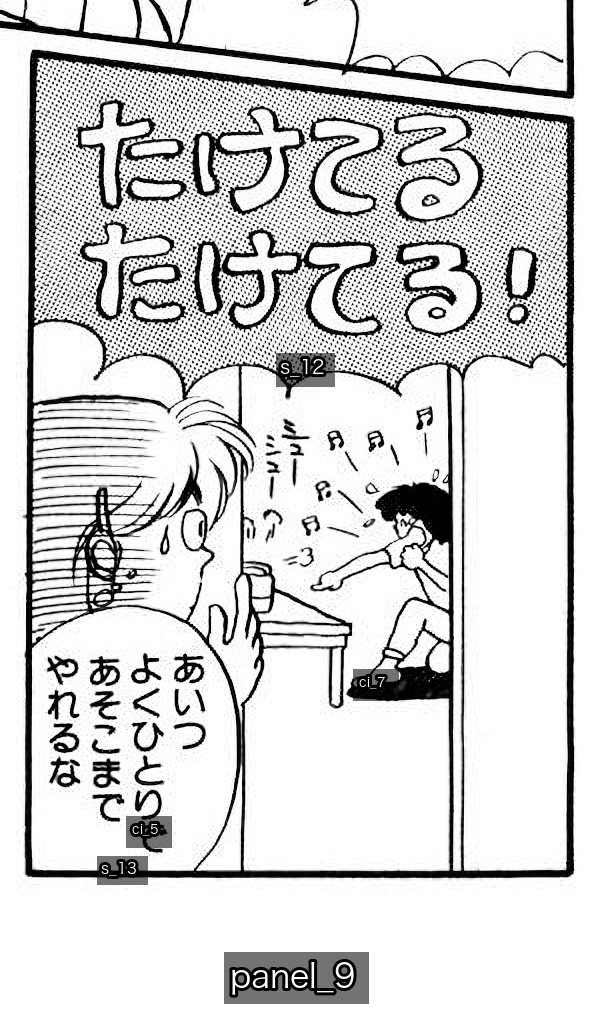
\includegraphics[width=\linewidth, valign=t]{pict/05/13_panel_panel_9.jpg}
       &
      % --- 右側：ID対応表 ---
      \small
      \adjustbox{valign=t}{%
         \renewcommand{\arraystretch}{1.35} % 日本語のために行間を少し広めにする
         % 左列(項目)は最小幅、右列(値)は折り返しあり
         \begin{tabular}{@{}l p{0.65\linewidth}@{}}
            \toprule
            \textbf{Attribute} & \textbf{Value / Description}                                               \\
            \midrule

            % --- Narrative Context (物語内容) ---
            \multicolumn{2}{@{}l}{\textit{\textbf{Narrative Context}}}                                      \\
            \quad ID           & \texttt{panel\_9}                                                          \\
            \quad Summary      & ご飯が炊けたことを踊って祝うあゆみと，それをドアの陰から見ているあさみ．                                       \\
            \quad Emotion      & \textbf{Joy} (あゆみ) vs \textbf{Confusion} (あさみ)                             \\

            % --- Cinematic (映像演出) ---
            \midrule
            \multicolumn{2}{@{}l}{\textit{\textbf{Cinematic \& Visuals}}}                                   \\
            \quad Shot         & Long Shot (LS), Eye-level                                                  \\
            \quad Composition  & 手前のあさみから，奥のあゆみへの視線誘導（Split depth）                                          \\

            % --- Graph Structure (IDによる構造化) ---
            % ここでIDを強調し、画像とのリンクを示す
            \midrule
            \multicolumn{2}{@{}l}{\textit{\textbf{Graph Structure (w/ IDs)}}}                               \\
            \quad Characters   & \texttt{ci\_7}: あゆみ (Dancing) \par \texttt{ci\_5}: あさみ (Watching)          \\
            \quad Speech       & \texttt{s\_12}: 歌唱・チャント (あゆみ) \par \texttt{s\_13}: 思考 (あさみ)                \\
            \quad Action Edge  & \texttt{ci\_5} (あさみ) $\xrightarrow{\text{observing}}$ \texttt{ci\_7} (あゆみ) \\

            \bottomrule
         \end{tabular}%
      }
   \end{tabular}

   \caption{IDラベルによりキャラクターの識別等状況が正確に構造化された例．画像内のIDタグである \texttt{ci} (Character Instance) はキャラクターを，\texttt{s} (Speech) はセリフを一意に識別しており，これらが右側の構造化データとして正しく対応付けられている(漫画:『愛さずにはいられない』©よし まさこ/集英社)．}
   \label{fig:panel_json_structure_with_id}
\end{figure}

\subsection{超解像度処理による認識性能の向上}\label{sec:super_resolution}

漫画画像には，
小さなコマや細密な描写が多く含まれており，
LVLM による内容理解において，
視認性の低さが性能低下の一因となる．
特に本研究では，
コマやセリフに ID ラベルを付記した画像を
入力として用いるため，
これらのラベルが
本来の描画内容を遮蔽し，かえって
視覚的理解を妨げるオクルージョンの問題が生じる．
そこで本研究では，
小さなコマの理解精度向上と，
ID ラベルによる視認性低下の抑制を目的として，
漫画画像に対する超解像度処理を導入した．

具体的には，
オープンソースの超解像モデルである
DRCT~\cite{DRCT} を用い，
元画像に対して
$\times 4$ の超解像処理を施した．
これにより，
細部の線画や文字情報が明瞭化され
LVLM による視覚的理解の安定化と，また ID が付記できるスペースを生み Visual Prompting の効果を高めることが可能となった．例えば，オクルージョンの問題を解決する手段としては，単純にフォントサイズを画像比率にあわせ縮小する方法も考えられるが，コマ画像のサイズによっては，描画できる最小フォントサイズに満たない場合もしばしば存在した．図~\ref{fig:super_resolution}に示すように，超解像度処理を施すことでこのような画像に対しても適度なサイズで ID ラベルを描画することが可能となった。

\begin{figure}[htbp]
   \centering
   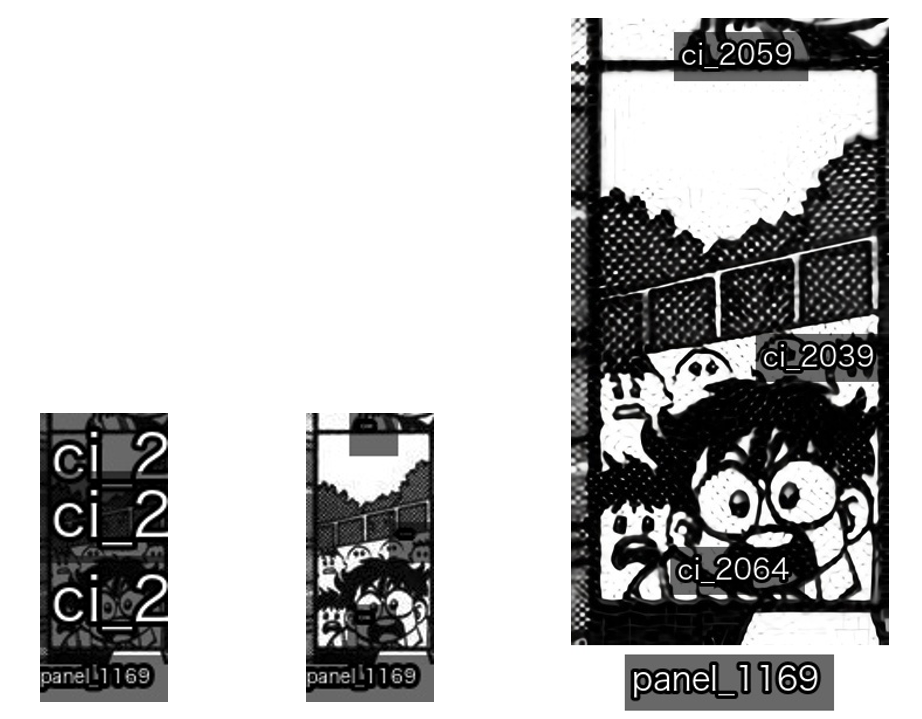
\includegraphics[width=0.5\textwidth]{pict/05/super_resolution.png}

   \caption{超解像度処理によるIDラベルの視認性が向上した例．左が最小フォントサイズを12ptに設定した画像，中央が画像比率にあわせ最小フォントサイズを設定した画像，右が超解像度処理を施し12ptのフォントサイズを設定した画像である．左は画像全体にオクルージョンが生じ，中央はラベル自体が付記できていないが，右は適度なサイズでIDラベルを描画できている(漫画:『うるとら★イレブン』©やぶの てんや, 渡辺 達也/集英社)．}
   \label{fig:super_resolution}
\end{figure}



一方で，
単純に高解像度化した画像を
そのまま LVLM に入力すると，
API の入力制約やタイル分割方式の影響により，
通常の画像であれば認識可能である
12pt 程度のフォントサイズであっても，
相対的に埋め込み領域が狭くなり，
ID ラベルが正しく認識されなくなる
問題が確認された．

この問題に対処するため，
本研究では，
$\times 4$ の超解像画像に対して，
線形輝度空間へ変換した上で
平均化処理を伴うダウンサンプリングを行い，
解像度を $\times \frac{1}{2}$ に縮小する手法も採用した．
この処理により，
元画像比で $\times 2$ 相当の解像度を持つ画像を生成し，
元画像の大きさや ID ラベルのサイズに応じて，
最も認識精度が高くなる
超解像度設定を選択できるようにした．

具体的な運用条件としては，
LVLM の API における1タイルが512×512ピクセルである
タイル分割方式を考慮し，
各コマ画像の超解像度化後の画像が
最大 4 タイル内で処理可能となるよう
画像サイズを調整した．
この条件下において，
ID ラベルの最小フォントサイズを
12pt 以上に維持しつつ，
描画内容へのオクルージョンが
最も小さくなる
超解像度設定および
入力コマ画像の選択を行った．

図\ref{fig:super_resolution_box}に，IDラベルの最小フォントサイズの縮小に伴う遮蔽率の変化と超解像度処理に伴う遮蔽率の比較を示す．これより，フォントサイズのを縮小する操作に比べると，2倍の超解像度処理でさえ、十分に遮蔽率の低減に優れた効果があることがわかる．

\begin{figure}[h]
   \centering
   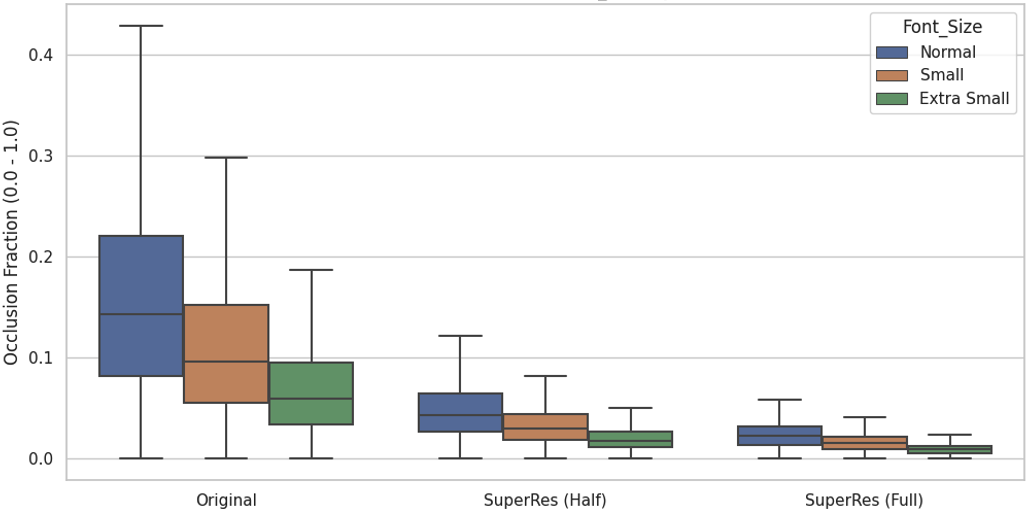
\includegraphics[width=\textwidth]{pict/05/super_resolution_box.png}

   \caption{IDラベルの最小フォントサイズの縮小に伴う遮蔽率の変化と超解像度処理に伴う遮蔽率の比較．Normal の最小フォントサイズは12ptで設定され，Small は9pt，Extra Small は6ptに設定された．SuperRes(Half)は２倍の超解像度処理画像，SuperRes(Full)は4倍の超解像度処理画像を表す．}
   \label{fig:super_resolution_box}
\end{figure}


以上の超解像度処理により，
小さなコマや細部表現の可読性が向上するとともに，
ID ラベルの付記が
漫画内容の理解を妨げる影響を
効果的に抑制できた．
この処理は，
後続の LVLM による
演出情報およびネーム構造の抽出を
安定して行うための
重要な前処理として機能している．

\subsection{文脈理解を促進する画像・セリフの入力}\label{sec:contextual_input}

漫画における演出や物語理解は，
単一の見開きやコマの内容のみから
完結するとは限らない．
特に，
キャラクターの関係性や感情の変化，
ギャグや伏線といった表現は，
前後の展開を踏まえて初めて
正しく解釈される場合が多い．
そのため，
対象とする見開き画像のみを
LVLM に入力した場合，
文脈依存の表現に対して
誤った解釈や表層的な記述が
生成されることが確認された．

そこで本研究では，
対象見開きに関する情報抽出に先立ち，
当該場面の前後文脈を
LVLM に明示的に与えることで，
漫画全体の流れを踏まえた理解を
促進する入力構成を採用した．
具体的には，
対象とする見開き画像に加え，
過去 9 ページ分の見開き画像，
および次の 1 ページ分の見開き画像を
併せて入力として与えた．
これにより，
直前までの展開や，
次に起こる反応を含めた
時間的連続性を
視覚的に参照可能とした．

さらに，
視覚情報だけでなく，
テキスト情報としても
物語文脈を補強するため，
過去ページに含まれる
全セリフを，
付与済みの読み順アノテーションに基づいて
正しい順序で入力した．
加えて，
それらのセリフ内容を
LVLM に要約させたテキストを併用し，
長距離文脈を簡潔に保持できるようにした．
この要約は，
対象見開きに至るまでの
物語状況やキャラクター関係を
高次の文脈として与える役割を果たす．

このように，
見開き画像，
個別コマ画像，
過去・未来ページの視覚情報，
および読み順付きセリフとその要約を
組み合わせて入力することで，
LVLM は，
単一ページに閉じた解釈ではなく，
物語全体の流れを踏まえた理解を
行えるようになる．
実際に，
対象見開きの概要文（Spread summary）には，
前段の出来事を前提とした記述や，
キャラクターの感情的変化を反映した表現が
含まれるようになり，
キャラクター名の誤同定や
関係性の取り違えも
大きく減少することを確認している．

以上の文脈情報を付与した入力構成は，
後続の演出情報および
ネーム構造の抽出において，
場面理解の一貫性と
記述の安定性を高める上で
重要な役割を果たしている．

図\ref{fig:contextual_summary_example}は，
文脈付与入力により，
見開き単体では読解困難な，過去のシーンの状況の理解が必要な場面で生成された概要分の抜粋を示す．このシーンでは，過去に登場した田中重夫という呼称に理解がないと読解できないが，文脈付与入力により正しく状況を理解することができている．

\begin{figure}[htbp]
   \centering
   \begin{tabular}{@{}p{0.48\linewidth}@{\hspace{1em}}p{0.48\linewidth}@{}}
      % --- 左側：画像 ---
      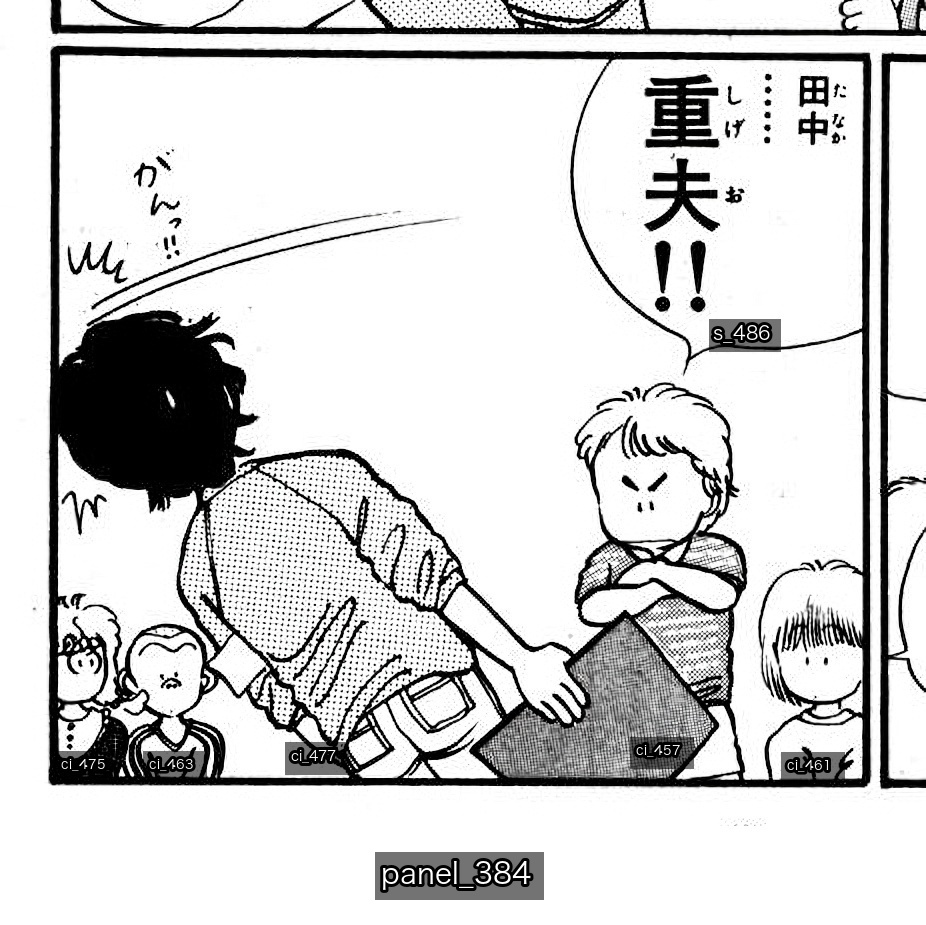
\includegraphics[width=\linewidth, valign=t]{pict/05/context_example.jpg}
       &
      % --- 右側：テキストボックス ---
      % ▼ ここでローカル設定（この図だけに適用）
      {
            \setlength{\fboxsep}{5mm} % 枠と文字の隙間を5mmに広げる（重要）
            \cornersize{0.3}          % 角の丸み具合
            \adjustbox{valign=t}{%
               \ovalbox{%
                  % 幅の計算は \fboxsep の変更に合わせて自動調整されます
                  \begin{minipage}[t]{\dimexpr\linewidth-2\fboxsep-2\fboxrule\relax}
                     \small
                     \linespread{0.75}\selectfont % 行間を広げて読みやすくする（モダン化）

                     \textbf{生成された summary の抜粋}\\[6pt]

                     「名前をいいなさい」と告げた。重夫は
                     「くっそお、きったねーっ！！」と
                     悔しがりながらも、観念したように
                     大声で叫んだ。
                     「ほれ！！名前」「田中……重夫！！」。
                     その名前を聞いた瞬間、歩の頭に衝撃が走る。
                     大家さんがいつも自分を呼ぶあの名前と
                     同じだったのだ。
                  \end{minipage}%
               }%
            }
         }
   \end{tabular}

   \caption{文脈付与入力により，見開き単体では理解が困難な場面で，過去の状況を正しく盛り込み正確な理解で summary が生成された例(漫画:『愛さずにはいられない』©よし まさこ/集英社)．}
   \label{fig:contextual_summary_example}
\end{figure}

\section{Manga109NameDataset の統計的特性}
\label{sec:name_statistics}

本節では，構築した
Manga109NameDataset の規模および構成要素の分布について，
各ノード種別および付与した属性の統計量を示す．以下では，
まずデータセット全体の規模を示し，
続いて各ノードに付与された情報の分布について，
ノード種別ごとに詳細を述べる．

\subsection{データセット全体の規模}
\label{sec:dataset_overview_stats}

表~\ref{tab:dataset_overview} に，
Manga109NameDataset に含まれる
見開き（Spread）ノード数，
および各ノード種別の総数と，
1 Spread あたりの平均数を示す．

\begin{table}[htbp]
   \centering
   \caption{Manga109NameDataset に含まれる各ノード種別の総数と 1 Spread あたりの平均数．なお Characterノードについても Spread ごとに集計した数を示す．}
   \label{tab:dataset_overview}
   \begin{tabular}{lrrrr}
      \hline
      \textbf{ノード種別}     & \textbf{総数} & \textbf{平均} \\
      \hline
      Spread             & 9{,}827     & 1.00        \\
      Panel              & 102{,}600   & 10.44       \\
      Character          & 39{,}478    & 4.02        \\
      Character Instance & 153{,}844   & 15.66       \\
      Speech             & 144{,}875   & 14.75       \\
      \hline
   \end{tabular}
\end{table}

表~\ref{tab:dataset_overview}に示された通り，本データセットは，Manga109Datasetに含まれる全見開き画像のうち，内部にコマ(Panel)を有するすべての画像を対象に構築されており，
合計 9{,}827 見開き分のデータを含む．
Manga109Datasetに含まれるすべてのコマの数は，全103,850コマであり，本データセットの構築においては，その98.8\%のコマに対して情報が抽出されたことを確認した．

\subsection{Spread ノードに付与された物語情報の統計}
\label{sec:spread_node_stats}
表~\ref{tab:spread_summary_stats} に，
Spread ノードに付与された
概要文（summary）の文字数分布に関する
統計量を示す．

\begin{table}[htbp]
   \centering
   \caption{Spread ノードに付与された summary の文字数の統計．}
   \label{tab:spread_summary_stats}
   \begin{tabular}{lr}
      \toprule
      \textbf{項目} & \textbf{数値} \\
      \midrule
      Spreadの総数   & 9{,}827     \\
      \cmidrule(lr){1-2}
      平均文字数       & 112.81      \\
      中央値文字数      & 94.00       \\
      最小文字数       & 12          \\
      最大文字数       & 702         \\
      標準偏差        & 79.07       \\
      \bottomrule
   \end{tabular}
\end{table}
平均で約 110 文字程度の概要文が付与されており，
見開き単位での物語内容や文脈を
簡潔かつ情報量を保った形で記述できていることを確認した．

\subsection{Panel ノードに付与された構成要素と演出属性の統計}
次に，Panel ノードに付与された構成要素と演出属性の統計を示す．

\paragraph{Panelのsummaryの文字数統計}
\label{sec:panel_summary_stats}
表~\ref{tab:panel_summary_stats} に，
Panel ノードに付与された概要文（summary）の
文字数統計を示す．summary は，各コマの視覚内容を簡潔に言語化したものであり，
大多数のコマに対して付与されている．

\begin{table}[htbp]
   \centering
   \caption{Panel ノードに付与された summary の文字数統計．}
   \label{tab:panel_summary_stats}
   \begin{tabular}{lr}
      \toprule
      \textbf{項目} & \textbf{数値} \\
      \midrule
      Panelの総数    & 102{,}600   \\
      \cmidrule(lr){1-2}
      平均文字数       & 79.20       \\
      中央値文字数      & 81.00       \\
      最小文字数       & 0           \\
      最大文字数       & 326         \\
      標準偏差        & 37.44       \\
      \bottomrule
   \end{tabular}
\end{table}

summary の文字数が 0 となったコマは，
全体の 2{,}058 / 102{,}600 コマ（約 2.01\%）に相当する．
これらの多くは，間（ま）やリズムを演出することを主目的とした
装飾的・演出的性格の強い空白コマであり，
その内容自体には summary として記述すべきものが見られないコマであった．平均すると約 79 文字程度の
summary が付与されており，その内容も十分な情報量を含んでいることを確認した．

\paragraph{物語上の役割と形状の分布}
各 Panel ノードには，
当該コマが物語の中で果たす役割を示す
役割属性が付与されており，また，その形状を示す
形状属性が付与されている．
表~\ref{tab:panel_roles_stats}，表~\ref{tab:panel_shape_stats}に，
付与されたすべての役割属性および形状属性
それぞれの出現頻度を示す．役割属性については、対話(dialogue\_exchange)や反応(reaction)といった人物中心の役割に加え，
間(pause\_or\_ma)や視線誘導(bridge\_or\_eye\_guidance)など，
漫画特有の演出機能を担うコマが
多数含まれていることが確認できた．また，コマ形状の属性を見ると，標準的なコマ形状に加え，
インセット(inset)や横長・縦長といった
多様なレイアウト表現が
数多く抽出されていることが確認できた．

% --- 1つ目のグループ：役割と形状 ---
\begin{table}[htbp]
   \centering

   % --- 左側：役割（行数が多い） ---
   \begin{minipage}[t]{0.48\linewidth}
      \centering
      % minipage内でキャプションをつける場合は \caption ではなく \subcaption や直接タイトルを書くか、
      % あるいは下記のように captionコマンドを使います
      \caption{役割属性の分布}
      \label{tab:panel_roles_stats}
      \begin{tabular}{lr}
         \toprule
         \textbf{役割属性}              & \textbf{数} \\
         \midrule
         dialogue\_exchange         & 29{,}993   \\
         reaction                   & 29{,}904   \\
         exposition                 & 23{,}113   \\
         showcase\_or\_impact       & 21{,}937   \\
         comedic                    & 21{,}666   \\
         pause\_or\_ma              & 19{,}179   \\
         action                     & 18{,}830   \\
         transition                 & 17{,}202   \\
         bridge\_or\_eye\_guidance  & 17{,}006   \\
         romance\_or\_introspection & 13{,}876   \\
         setting\_or\_background    & 9{,}074    \\
         hook\_or\_intro            & 8{,}965    \\
         time\_progression          & 5{,}068    \\
         flashback                  & 1{,}591    \\
         \bottomrule
      \end{tabular}
   \end{minipage}
   \hfill % 左右の間のスペースを自動調整
   % --- 右側：形状（行数が少ない） ---
   \begin{minipage}[t]{0.48\linewidth}
      \centering
      \caption{コマ形状の分布}
      \label{tab:panel_shape_stats}
      \begin{tabular}{lr}
         \toprule
         \textbf{コマ形状属性}      & \textbf{数} \\
         \midrule
         inset                & 45{,}591   \\
         horizontal\_yokogoma & 22{,}952   \\
         standard             & 17{,}951   \\
         vertical\_tategoma   & 15{,}394   \\
         double\_spread       & 552        \\
         splash\_full\_bleed  & 160        \\
         \bottomrule
      \end{tabular}

      % 右側の表が短くて下の余白が気になる場合、ここに解説文を入れて埋めるテクニックもあります。
      \vspace{1em}
   \end{minipage}
\end{table}


\paragraph{カメラ距離およびアングルの分布}
Panel ノードには，
演出上の視点を表す属性として，
カメラ距離およびアングルが付与されている．表~\ref{tab:panel_camera_distance_stats} および
表~\ref{tab:panel_camera_angle_stats} に，
それぞれの分布を示す．目線高さ（eye\_level）を基準とした自然な構図が多数を占める一方で，
角度や距離の変化による演出表現も
幅広く含まれており，
本データセットが
多様な視覚的演出を内包していることが確認できた．


% --- 2つ目のグループ：カメラ距離とアングル（高さが揃ってきれい） ---
\begin{table}[htbp]
   \centering
   % --- 左側：カメラ距離 ---
   \begin{minipage}[t]{0.48\linewidth}
      \centering
      \caption{カメラ距離の分布}
      \label{tab:panel_camera_distance_stats}
      \begin{tabular}{lr}
         \toprule
         \textbf{カメラ距離属性} & \textbf{数} \\
         \midrule
         MS               & 29{,}572   \\
         CU               & 26{,}226   \\
         MCU              & 16{,}181   \\
         LS               & 15{,}249   \\
         ECU              & 5{,}728    \\
         establishing     & 2{,}238    \\
         XLS              & 1{,}780    \\
         MLS              & 1{,}502    \\
         XCU              & 671        \\
         \bottomrule
      \end{tabular}
   \end{minipage}
   \hfill
   % --- 右側：カメラアングル ---
   \begin{minipage}[t]{0.48\linewidth}
      \centering
      \caption{カメラアングルの分布}
      \label{tab:panel_camera_angle_stats}
      \begin{tabular}{lr}
         \toprule
         \textbf{カメラアングル属性} & \textbf{数} \\
         \midrule
         eye\_level         & 66{,}468   \\
         low                & 7{,}343    \\
         profile\_side      & 7{,}313    \\
         level              & 6{,}699    \\
         high               & 5{,}697    \\
         top\_shot          & 2{,}513    \\
         dutch\_tilt        & 2{,}225    \\
         back\_view         & 1{,}663    \\
         bird\_eye          & 223        \\
         worm\_eye          & 76         \\
         \bottomrule
      \end{tabular}
   \end{minipage}
\end{table}

\subsection{Character ノードの統計的特性}
\label{sec:character_node_stats}
次に，
Character ノードの統計的特性を示す．
Character ノードは，
物語中に登場する人物そのものを表すノードであり，
Panel や Speech のように見開き単位で生成されるのではなく，
作品全体を通して一貫して定義される点に特徴がある．
本データセットでは，
Manga109Dataset に含まれる各作品に登場する人物を統合し，
合計 5{,}375 人のユニークなキャラクターが定義されている．

\paragraph{人物プロフィール記述の統計}
Character ノードには，
人物の性格や背景，物語上の立ち位置を記述した
プロフィール文（profile）が付与される．
表~\ref{tab:character_profile_stats} に，
profile の文字数分布に関する統計量を示す．

\begin{table}[htbp]
   \centering
   \caption{Character ノードに付与された profile の文字数統計．}
   \label{tab:character_profile_stats}
   \begin{tabular}{lr}
      \toprule
      \textbf{項目} & \textbf{値} \\
      \midrule
      キャラクター総数    & 5{,}375    \\
      \cmidrule(lr){1-2}
      平均文字数       & 71.78      \\
      中央値文字数      & 71.00      \\
      最小文字数       & 0          \\
      最大文字数       & 153        \\
      標準偏差        & 28.24      \\
      \bottomrule
   \end{tabular}
\end{table}

profile が空であるキャラクターは
21体（全体の 0.39\%）存在するが，
これらのキャラクターの多くは，作品にほとんど関与しないモブキャラであることが確認できている．平均文字数はおよそ72文字で，そのキャラクターのプロフィールを表す言語情報が適切に付与されていることを確認した．

Character ノードには，
物語における役割や重要度を表す属性が付与されている．
これらの分布を表~\ref{tab:character_role_stats} および
表~\ref{tab:character_importance_stats} に示す．
表~\ref{tab:character_role_stats} より，
主人公（protagonist）や副主人公（deuteragonist）など，
物語の中心人物に相当する役割に加え，
支援者（suppo  rting）や背景キャラクター（background）など，
補助的・周辺的な役割を担うキャラクターの描写についても属性の抽出が行えていることが確認できた．また，表~\ref{tab:character_importance_stats}に示される重要度分布では，main，sub，minor が広く分布しており，少数の主要キャラクター
を軸としつつ，多数の準主要・脇役キャラクターが物語を構成している典型的な漫画作品の構造が確認
できた．このような重要度の階層性は，キャラクターごとの描写密度や演出上の扱いの違いを学習・分
析する上で重要な情報となる．


\begin{table}[htbp]
   \centering
   % --- 左：role ---
   \begin{minipage}[t]{0.48\linewidth}
      \centering
      \caption{Character role の分布}
      \label{tab:character_role_stats}
      \begin{tabular}{lr}
         \toprule
         \textbf{役割属性}  & \textbf{数} \\
         \midrule
         protagonist    & 9{,}008    \\
         supporting     & 4{,}711    \\
         background     & 4{,}515    \\
         deuteragonist  & 4{,}443    \\
         ally           & 4{,}255    \\
         antagonist     & 3{,}218    \\
         love\_interest & 2{,}131    \\
         mentor         & 1{,}561    \\
         rival          & 1{,}278    \\
         family         & 1{,}206    \\
         tritagonist    & 1{,}194    \\
         authority      & 1{,}113    \\
         comic\_relief  & 654        \\
         narrator       & 183        \\
         unknown        & 27         \\
         \bottomrule
      \end{tabular}
   \end{minipage}
   \hfill
   % --- 右：importance ---
   \begin{minipage}[t]{0.48\linewidth}
      \centering
      \caption{Character importance の分布}
      \label{tab:character_importance_stats}
      \begin{tabular}{lr}
         \toprule
         \textbf{重要度属性} & \textbf{数} \\
         \midrule
         main           & 21{,}455   \\
         sub            & 9{,}655    \\
         minor          & 8{,}281    \\
         cameo          & 81         \\
         unknown        & 25         \\
         \bottomrule
      \end{tabular}
   \end{minipage}
\end{table}

\paragraph{物語的属性および主人公との関係}
さらに，
Character ノードには，物語的立場を表す属性および
主人公との関係を示す属性が付与されている．
これらの分布を表~\ref{tab:character_alignment_stats}および \ref{tab:character_relation_stats} に示す．表~\ref{tab:character_alignment_stats}より物語立場の多くはheroと判定されていることがわかる．この属性

% \begin{table}[htbp]
% \centering
% % --- 左：alignment ---
% \begin{minipage}[t]{0.48\linewidth}
%    \centering
%    \caption{Character alignment の分布}
%    \label{tab:character_alignment_stats}
%    \begin{tabular}{lr}
%       \toprule
%       \textbf{alignment} & \textbf{数} \\
%       \midrule
%       hero               & 22{,}652   \\
%       neutral            & 13{,}704   \\
%       villain            & 2{,}845    \\
%       unknown            & 296        \\
%       \bottomrule
%    \end{tabular}
% \end{minipage}

% --- 右：relation ---
% \begin{minipage}[t]{0.48\linewidth}
% \centering
%    \caption{relation\_to\_protagonist の分布}
%    \label{tab:character_relation_stats}
%    \begin{tabular}{lr}
%       \toprule
%       \textbf{relation\_to\_protagonist} & \textbf{数} \\
%       \midrule
%       ally                               & 8{,}981    \\
%       self                               & 8{,}560    \\
%       other                              & 8{,}087    \\
%       love\_interest                     & 3{,}216    \\
%       enemy                              & 2{,}931    \\
%       family                             & 2{,}870    \\
%       mentor                             & 1{,}279    \\
%       rival                              & 1{,}243    \\
%       authority                          & 966        \\
%       subordinate                        & 690        \\
%       unknown                            & 674        \\
%       \bottomrule
%    \end{tabular}
%    % \end{minipage}
% \end{table}

以上より，
Manga109NameDataset における Character ノードは，
人物像を表す自由記述と，
物語構造を反映した複数の属性を併せ持つことで，
後続の演出解析やネーム生成において
物語的整合性を保持するための
基盤情報として機能する．

\subsection{Character Instance ノードの統計的特性}
\label{sec:character_instance_node_stats}
次に，
Character Instance ノードの統計的特性を示す．
Character Instance ノードは，
特定のコマ内におけるキャラクターの具体的な描写を表すノードであり，
姿勢・動作・感情といった視覚的および演出的な情報を担う．
同一の Character ノードが複数のコマに登場する場合でも，
それぞれの描写は独立した Character Instance として定義されるため，
本ノードはデータセット内で最も出現数の多いノード種別となっている．
本データセットでは，
合計 153{,}867 個の Character Instance ノードが含まれている．

\paragraph{自由記述属性（姿勢・動作・感情）の文字数分布}
Character Instance ノードには，
描画内容を言語的に記述した自由記述属性として，姿勢の記述，行動の記述，感情の記述の3項目が付与されている．表~\ref{tab:ci_text_stats}に，各属性の文字数分布に関する統計量を示す．

\begin{table}[htbp]
   \centering
   \caption{Character Instance ノードに付与された自由記述属性の文字数統計}
   \label{tab:ci_text_stats}
   \begin{minipage}[t]{0.32\linewidth}
      \centering
      \caption*{姿勢}
      \begin{tabular}{lr}
         \toprule
         項目     & 値     \\
         \midrule
         平均文字数  & 38.69 \\
         中央値文字数 & 41.00 \\
         最小文字数  & 0     \\
         最大文字数  & 178   \\
         標準偏差   & 19.68 \\
         \bottomrule
      \end{tabular}
   \end{minipage}
   \hfill
   \begin{minipage}[t]{0.32\linewidth}
      \centering
      \caption*{行動}
      \begin{tabular}{lr}
         \toprule
         項目     & 値     \\
         \midrule
         平均文字数  & 44.31 \\
         中央値文字数 & 48.00 \\
         最小文字数  & 0     \\
         最大文字数  & 218   \\
         標準偏差   & 27.95 \\
         \bottomrule
      \end{tabular}
   \end{minipage}
   \hfill
   \begin{minipage}[t]{0.32\linewidth}
      \centering
      \caption*{感情}
      \begin{tabular}{lr}
         \toprule
         項目     & 値     \\
         \midrule
         平均文字数  & 21.46 \\
         中央値文字数 & 23.00 \\
         最小文字数  & 0     \\
         最大文字数  & 97    \\
         標準偏差   & 10.90 \\
         \bottomrule
      \end{tabular}
   \end{minipage}
\end{table}

2,687体(全体の約1.75\%)の描画は，
姿勢，行動，感情のいずれも空白であったが，これらの多くはキャラクターが背景として小さく描かれている場合などであることを確認した．
平均文字数もそれぞれの項目を記述するのに十分な長さであることを確認した．


\paragraph{姿勢・動作・感情に関する離散属性の分布}
自由記述に加え，
Character Instance ノードには，
姿勢・動作・感情を離散的なカテゴリとして表現する属性が付与されている．また加えて，その描画が顔を中心としているか，それとも体を中心としているかを表す属性も付与されている．
これらの属性は，
自然言語記述を補完する構造化情報として機能する．
表~\ref{tab:ci_pose_enum_stats}，表~\ref{tab:ci_action_enum_stats}，表~\ref{tab:ci_emotion_enum_stats}，表~\ref{tab:ci_face_body_enum_stats}，に，
各属性値の分布を示す．

\begin{table}[htbp]
   \centering
   % --- 上段 ---
   \begin{minipage}[t]{0.48\linewidth}
      \centering
      \caption{姿勢属性の分布}
      \label{tab:ci_pose_enum_stats}
      \begin{tabular}{lr}
         \toprule
         姿勢属性          & 数        \\
         \midrule
         head\_shot    & 31{,}905 \\
         upper\_body   & 22{,}865 \\
         partial\_body & 12{,}073 \\
         profile       & 8{,}536  \\
         standing      & 7{,}649  \\
         back\_view    & 5{,}642  \\
         leaning       & 3{,}366  \\
         sitting       & 3{,}087  \\
         full\_body    & 2{,}166  \\
         walking       & 1{,}132  \\
         dynamic       & 1{,}093  \\
         running       & 813      \\
         background    & 643      \\
         lying\_down   & 486      \\
         falling       & 352      \\
         crouching     & 304      \\
         silhouette    & 228      \\
         floating      & 199      \\
         jumping       & 165      \\
         lying\_prone  & 131      \\
         lying\_back   & 93       \\
         chibi         & 59       \\
         all\_fours    & 44       \\
         split         & 38       \\
         leg\_up       & 35       \\
         restrained    & 16       \\
         backbend      & 13       \\
         lying\_side   & 5        \\
         kneeling      & 4        \\
         straddling    & 3        \\
         crossed\_legs & 1        \\
         other         & 48{,}022 \\
         \bottomrule
      \end{tabular}
   \end{minipage}
   \hfill
   \begin{minipage}[t]{0.48\linewidth}
      \centering
      \caption{行動属性の分布}
      \label{tab:ci_action_enum_stats}
      \begin{tabular}{lr}
         \toprule
         行動属性               & 数        \\
         \midrule
         speak              & 30{,}012 \\
         watch              & 23{,}271 \\
         object\_handling   & 6{,}057  \\
         listen             & 4{,}770  \\
         stand              & 3{,}497  \\
         interact           & 2{,}806  \\
         perform            & 2{,}604  \\
         move               & 2{,}523  \\
         consume            & 2{,}152  \\
         ask                & 2{,}152  \\
         fight              & 1{,}992  \\
         gesture            & 1{,}991  \\
         think              & 1{,}910  \\
         walk               & 1{,}902  \\
         explain            & 1{,}861  \\
         physical\_response & 1{,}712  \\
         run                & 1{,}611  \\
         sit                & 1{,}586  \\
         fall               & 1{,}226  \\
         chase              & 1{,}012  \\
         sleep              & 864      \\
         wait               & 862      \\
         cheer              & 798      \\
         defend             & 747      \\
         smile              & 638      \\
         hide               & 479      \\
         laugh              & 405      \\
         fly                & 379      \\
         greet              & 352      \\
         cry                & 332      \\
         tremble            & 280      \\
         other              & 48{,}385 \\
         \bottomrule
      \end{tabular}
   \end{minipage}
\end{table}

\begin{table}[htbp]
   \centering
   % --- 下段 ---
   \begin{minipage}[t]{0.48\linewidth}
      \centering
      \caption{感情属性の分布}
      \label{tab:ci_emotion_enum_stats}
      \begin{tabular}{lr}
         \toprule
         感情属性         & 数        \\
         \midrule
         anxious      & 21{,}546 \\
         neutral      & 12{,}933 \\
         shocked      & 9{,}579  \\
         happy        & 9{,}338  \\
         calm         & 6{,}603  \\
         afraid       & 6{,}216  \\
         angry        & 5{,}972  \\
         sad          & 5{,}335  \\
         surprised    & 5{,}315  \\
         determined   & 5{,}283  \\
         confused     & 3{,}895  \\
         excited      & 3{,}815  \\
         confident    & 3{,}345  \\
         serious      & 3{,}060  \\
         frustrated   & 2{,}448  \\
         worried      & 2{,}318  \\
         curious      & 2{,}106  \\
         desperate    & 1{,}405  \\
         tired        & 1{,}146  \\
         affectionate & 955      \\
         hostile      & 900      \\
         disgusted    & 761      \\
         embarrassed  & 698      \\
         suspicious   & 672      \\
         thoughtful   & 572      \\
         bored        & 102      \\
         other        & 34{,}850 \\
         \bottomrule
      \end{tabular}
   \end{minipage}
   \hfill
   \begin{minipage}[t]{0.48\linewidth}
      \centering
      \caption{face\_body属性の分布}
      \label{tab:ci_face_body_enum_stats}
      \begin{tabular}{lr}
         \toprule
         face\_body属性 & 数         \\
         \midrule
         face\&body   & 113{,}740 \\
         body\_only   & 39{,}191  \\
         face\_only   & 936       \\
         \bottomrule
      \end{tabular}
   \end{minipage}
\end{table}

これらの分布から，
Character Instance に付与された離散属性は，
漫画表現において頻出する描画様式や行動・感情を
幅広くカバーできていることを確認した．
姿勢属性（表~\ref{tab:ci_pose_enum_stats}）では，
head\_shot や upper\_body といった
顔や上半身を中心とした描写が多く，
感情表現や対話を重視する漫画的演出の傾向が反映されていることが確認できた．
行動属性（表~\ref{tab:ci_action_enum_stats}）においては，
speak，watch，listen など，
会話や相互注視に関わる行動が高頻度で現れており，
キャラクター間の関係性が
物語進行の中心となっていることが読み取れる．
感情属性（表~\ref{tab:ci_emotion_enum_stats}）では，
anxious，neutral，shocked，happy といった
物語展開上重要な感情状態が多く含まれていることが確認できた．
さらに，
face\_body 属性（表~\ref{tab:ci_face_body_enum_stats}）より，
顔と身体の両方を含む描写が大半を占める一方で，
顔のみ・身体のみの描写も一定数存在し，
演出上の強調や省略が
構造的に表現されていることを確認した．

以上より，
Character Instance ノードは，
詳細な自然言語記述と
多様な離散的属性を併せ持つことで，
コマ内におけるキャラクター表現を
多角的に捉えるための情報構造を形成していることが確認できた．

\subsection{Speech ノードの統計的特性}
\label{sec:speech_node_stats}
次に，
Speech ノードの統計的特性を示す．
Speech ノードは，
漫画における吹き出しや文字表現を単位として，
発話内容およびその機能的役割を表すノードである．発話内容はManga109Datasetに含まれている値をそのまま用いて，本データセットの構築においては，機能的な役割を付与した．
各 Speech ノードは，
特定のコマおよびキャラクターインスタンスと結び付けられる．
本データセットには，
合計 141{,}879 個の Speech ノードが含まれている．
\paragraph{発話テキストの文字数分布}
Manga109Datasetに含まれる発話内容をそのまま格納したテキスト属性についてその統計量を表~\ref{tab:speech_text_stats} に示す．

\begin{table}[htbp]
   \centering
   \caption{Speech ノードに付与された発話テキストの文字数統計}
   \label{tab:speech_text_stats}
   \begin{tabular}{lr}
      \toprule
      項目     & 値     \\
      \midrule
      平均文字数  & 13.79 \\
      中央値文字数 & 11.00 \\
      最小文字数  & 1     \\
      最大文字数  & 273   \\
      標準偏差   & 10.87 \\
      \bottomrule
   \end{tabular}
\end{table}

\paragraph{発話種別の分布}
次に，Speech ノードに付与した，
発話の機能や性質を表す
離散的な属性，発話種別属性についてその分布を表~\ref{tab:speech_type_enum_stats} に示す．

\begin{table}[htbp]
   \centering
   \caption{Speech ノードにおける発話種別属性の分布}
   \label{tab:speech_type_enum_stats}
   \begin{tabular}{lr}
      \toprule
      発話種別属性           & 数        \\
      \midrule
      dialogue         & 85{,}563 \\
      shout\_reaction  & 29{,}534 \\
      inner\_monologue & 12{,}475 \\
      narration        & 6{,}702  \\
      sound\_effect    & 1{,}567  \\
      broadcast        & 1{,}534  \\
      other            & 1{,}148  \\
      ambient\_text    & 1{,}002  \\
      signage          & 971      \\
      meta\_commentary & 921      \\
      song\_or\_chant  & 462      \\
      \bottomrule
   \end{tabular}
\end{table}

対話（\texttt{dialogue}）が全体の過半数を占める一方で，
感嘆や反応を表す \texttt{shout\_reaction}，
内面描写を担う \texttt{inner\_monologue}，
場面説明を行う \texttt{narration} など，
多様な発話機能が含まれていることが分かる．
また，
擬音語や環境音を表す \texttt{sound\_effect}，
標識や看板などの \texttt{signage} も明示的に区別されており，
漫画特有の文字表現を幅広く網羅できていることが確認できた．

以上より，
Speech ノードは，
短い会話から説明的テキストまでを包含する
多様な言語表現を保持しており，
視覚表現と結び付いた物語構造を解析する上で
重要な役割を果たす．

\subsection{キャラクター間相互作用を表す Action Edge の統計}
\label{sec:action_edge_stats}

Action Edge は，
同一コマ内あるいは連続するコマ内において，
キャラクターインスタンス同士がどのような相互作用を持つかを，
自由記述形式で表現したエッジである．
これらは，
視線の向き，接触，攻撃，援助といった
明示的な行動関係が記述されている．

表~\ref{tab:action_edge_length_stats} に，
Action Edge に付与された記述文の文字数に関する
統計量を示す．
本データセットには，
合計 38{,}633 件の Action Edge が含まれており，

\begin{table}[htbp]
   \centering
   \caption{Action Edge に付与された相互作用記述の文字数統計}
   \label{tab:action_edge_length_stats}
   \begin{tabular}{lr}
      \toprule
      \textbf{項目}    & \textbf{値} \\
      \midrule
      Action Edge 総数 & 38{,}633   \\
      \cmidrule(lr){1-2}
      最小文字数          & 6          \\
      最大文字数          & 86         \\
      平均文字数          & 32.90      \\
      中央値文字数         & 34.00      \\
      \bottomrule
   \end{tabular}
\end{table}

このような記述長の分布から，
相互作用が
「誰が誰に何をしているか」
という最小限の意味単位として
安定して抽出されていることが確認できた．
Action Edge は，
キャラクター配置や視線関係，
対話構造といった情報と組み合わせることで，
ネーム全体の演出的関係性を
グラフ構造上で補完する役割を果たす．

\section{構造化データの可視化例}\label{sec:name_sample}
本節では，
図~\ref{fig:sample_manga} に示す一つの見開き漫画を入力として，
本研究の手法により段階的に抽出・構造化されたManga109NameDatasetにおける1サンプル
データの可視化の具体例を示す．

\begin{figure}[p]
   \centering
   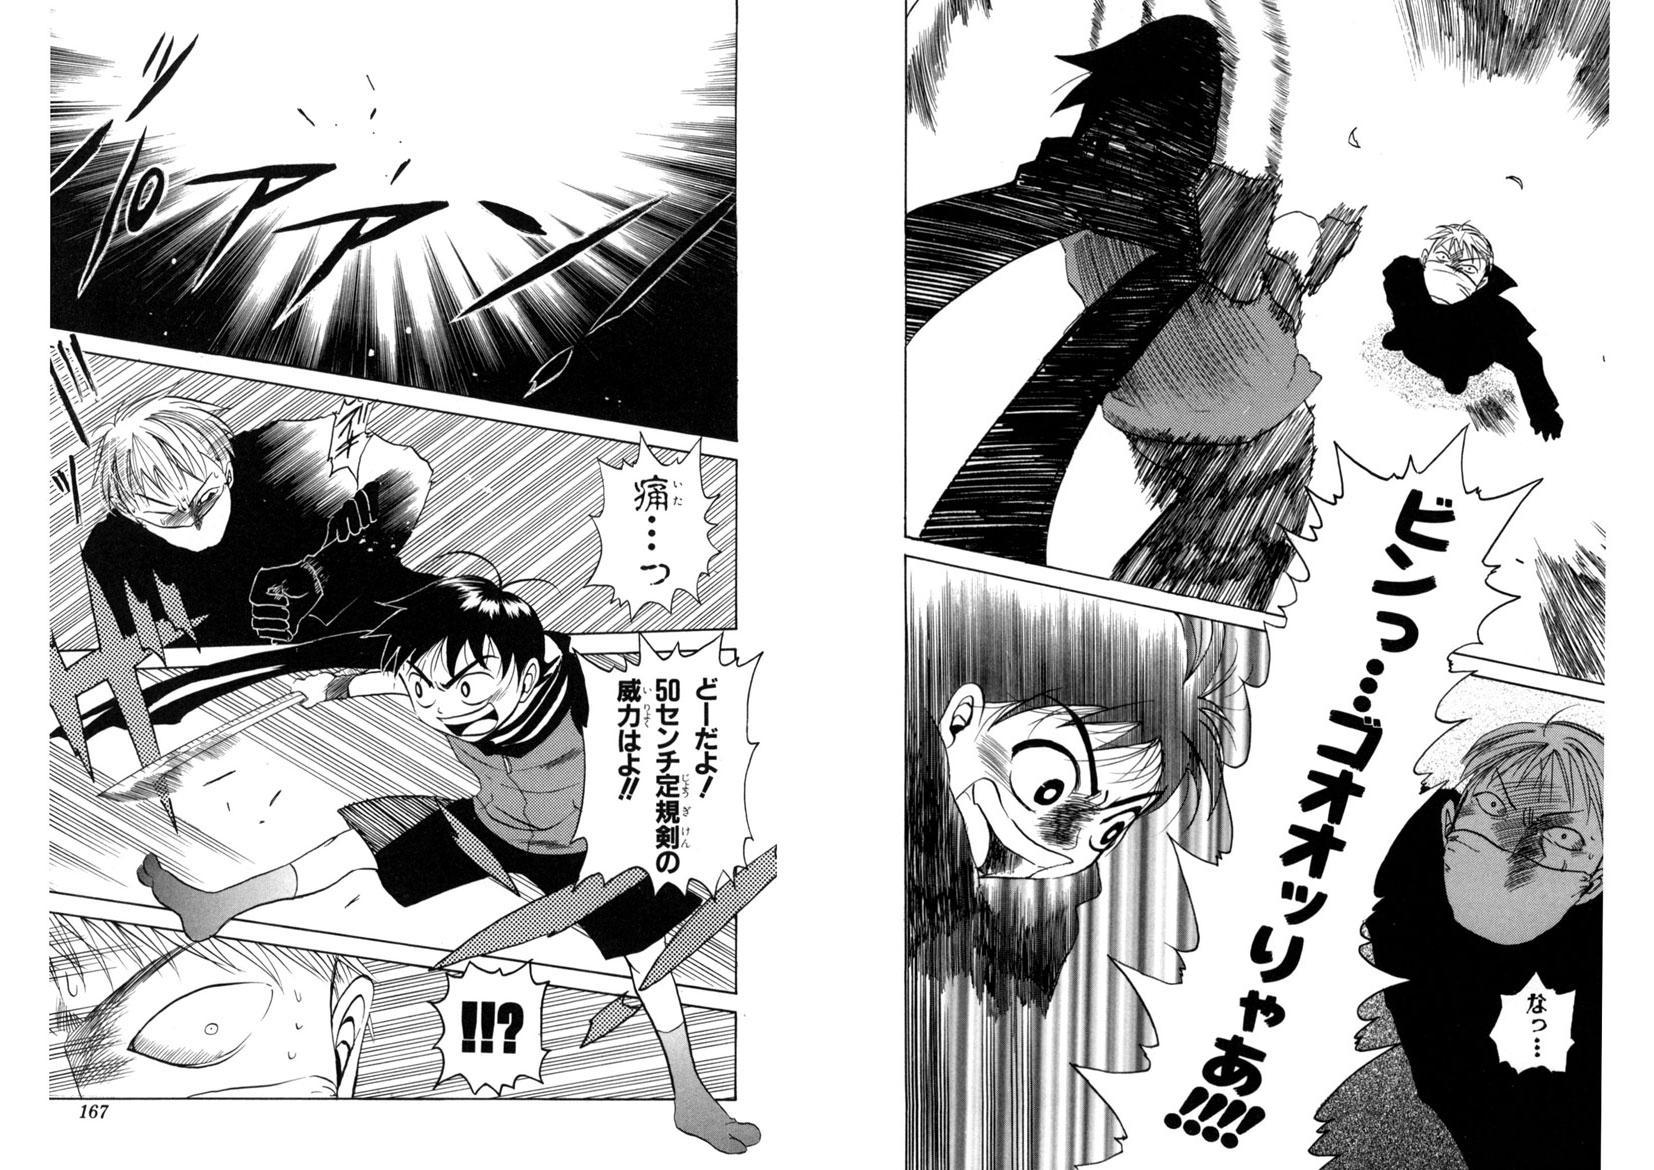
\includegraphics[width=0.8\textwidth]{pict/05/samples_manga.jpg}
   \caption{本節で例示する Manga109NameDataset の入力見開き画像(漫画:『	あっけら貫刃帖』©小林 ゆき/集英社)．}
   \label{fig:sample_manga}
\end{figure}

\begin{figure}[p]
   \centering
   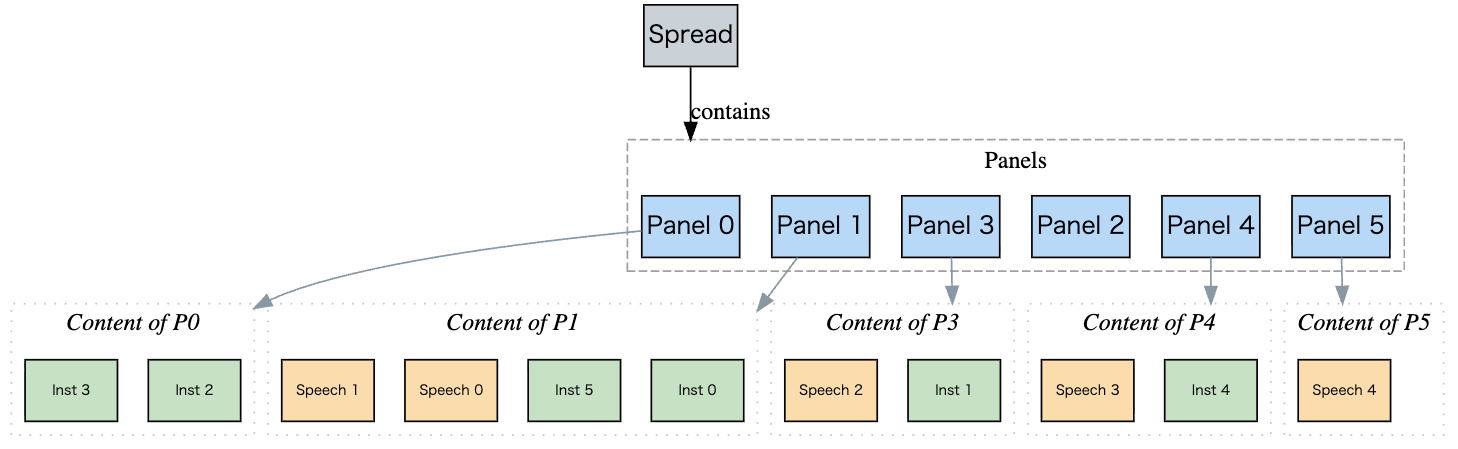
\includegraphics[width=\textwidth]{pict/05/samples_hierarcny.png}
   \caption{構築された階層構造の例．InstはCharacterInstanceノードを表す．}
   \label{fig:sample_hierarchy}
\end{figure}

\begin{figure}[p]
   \centering
   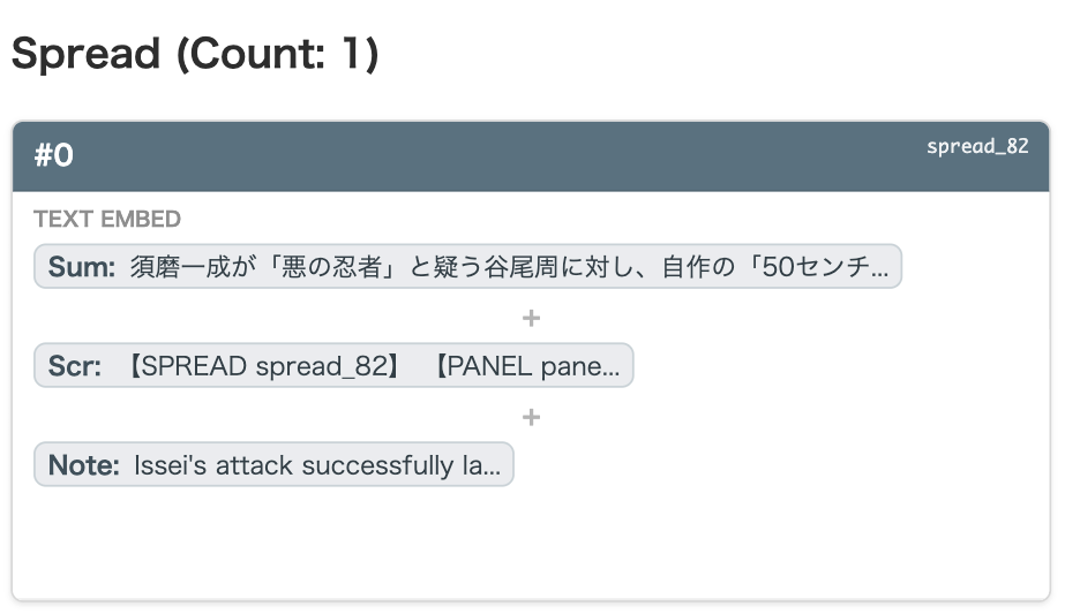
\includegraphics[width=0.60\textwidth]{pict/05/samples_spread.png}
   \caption{Spread ノードの例．}
   \label{fig:sample_spread}
\end{figure}

\begin{figure}[p]
   \centering
   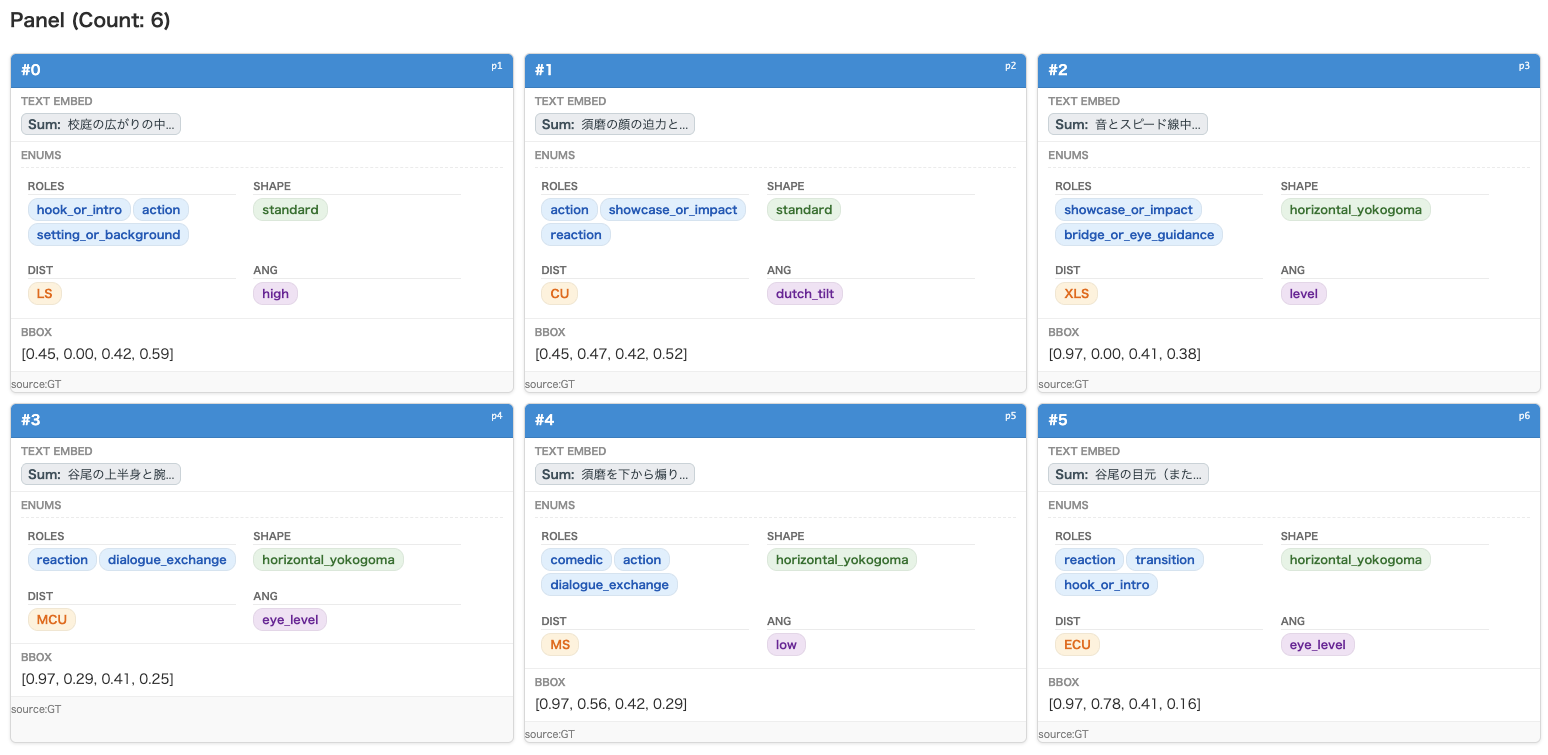
\includegraphics[width=\textwidth]{pict/05/samples_panels.png}
   \caption{Panel ノードの例．}
   \label{fig:sample_panels}
\end{figure}

\begin{figure}[p]
   \centering
   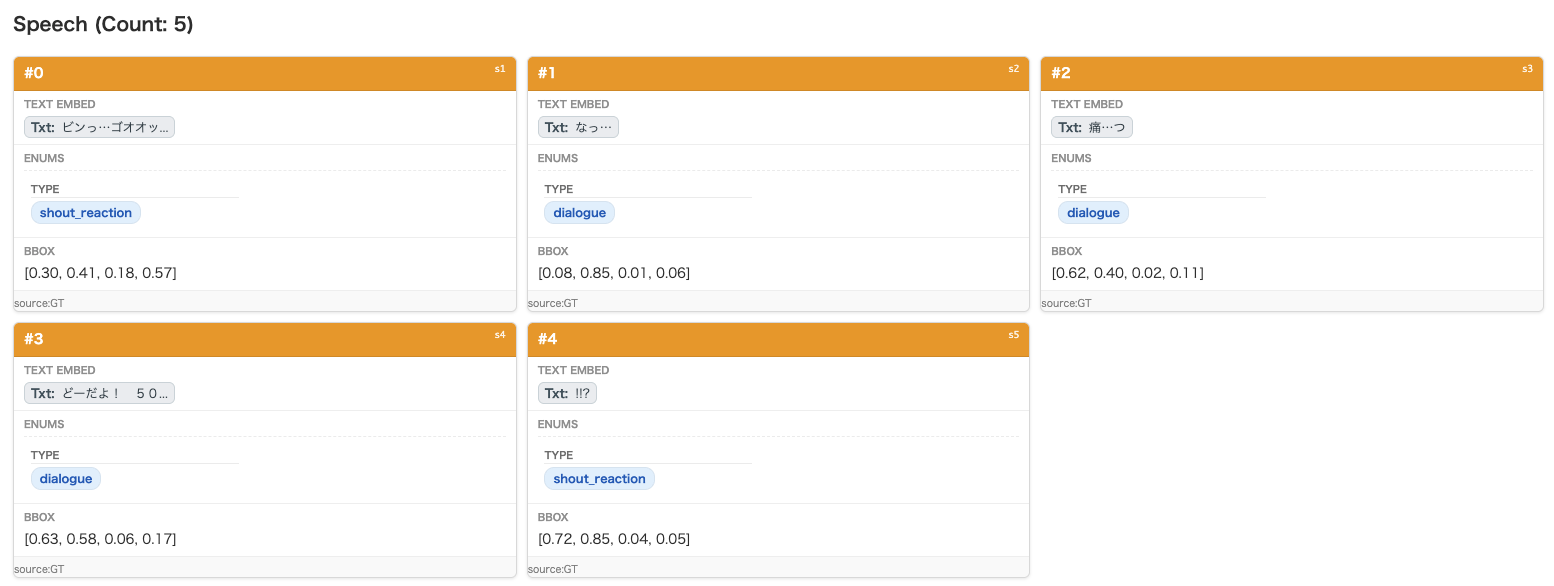
\includegraphics[width=\textwidth]{pict/05/samples_speech.png}
   \caption{Speech ノードにの例．}
   \label{fig:sample_speech}
\end{figure}

\begin{figure}[p]
   \centering
   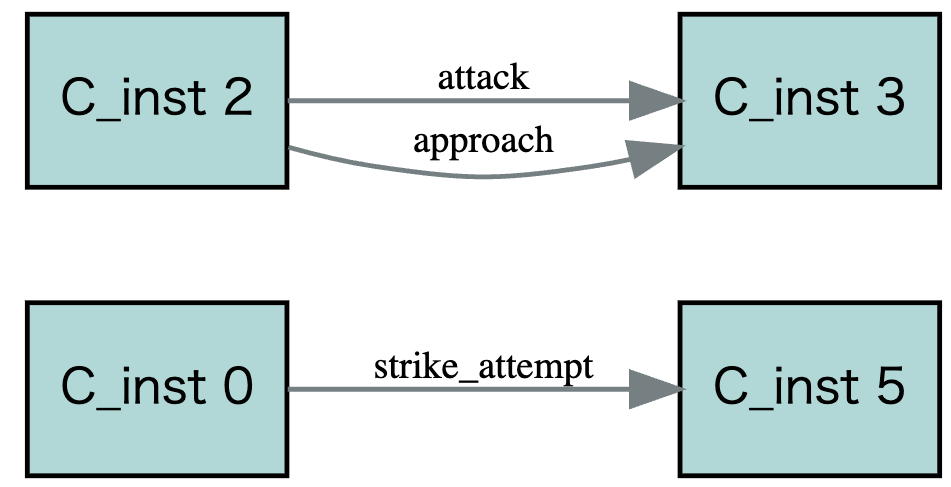
\includegraphics[width=0.50\textwidth]{pict/05/samples_action_edge.png}
   \caption{キャラクターインスタンス間の相互作用（Action Edge）の例．C\_instはCharacterInstanceノードを表す．}
   \label{fig:sample_action_edge}
\end{figure}
\begin{figure}[p]
   \centering
   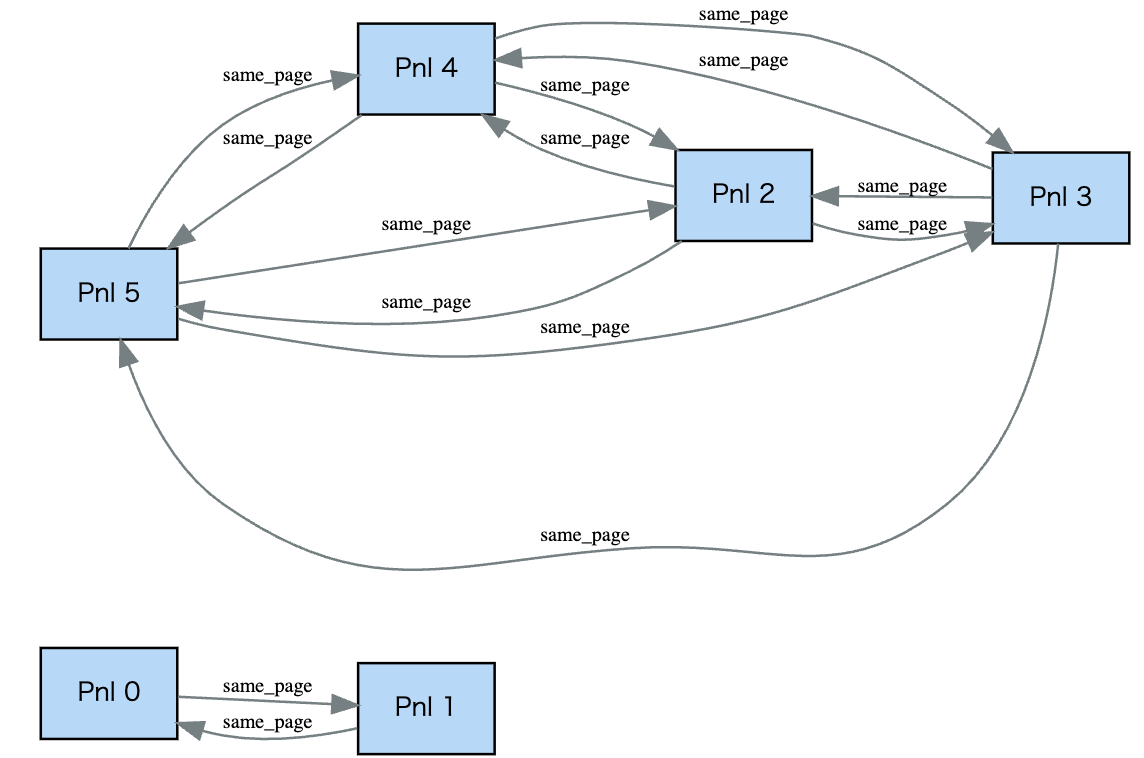
\includegraphics[width=\textwidth]{pict/05/samples_samepages.png}
   \caption{同一ページ内のPanel間の参照関係の例．PnlはPanelノードを表す．}
   \label{fig:sample_samepages}
\end{figure}
\begin{figure}[p]
   \centering
   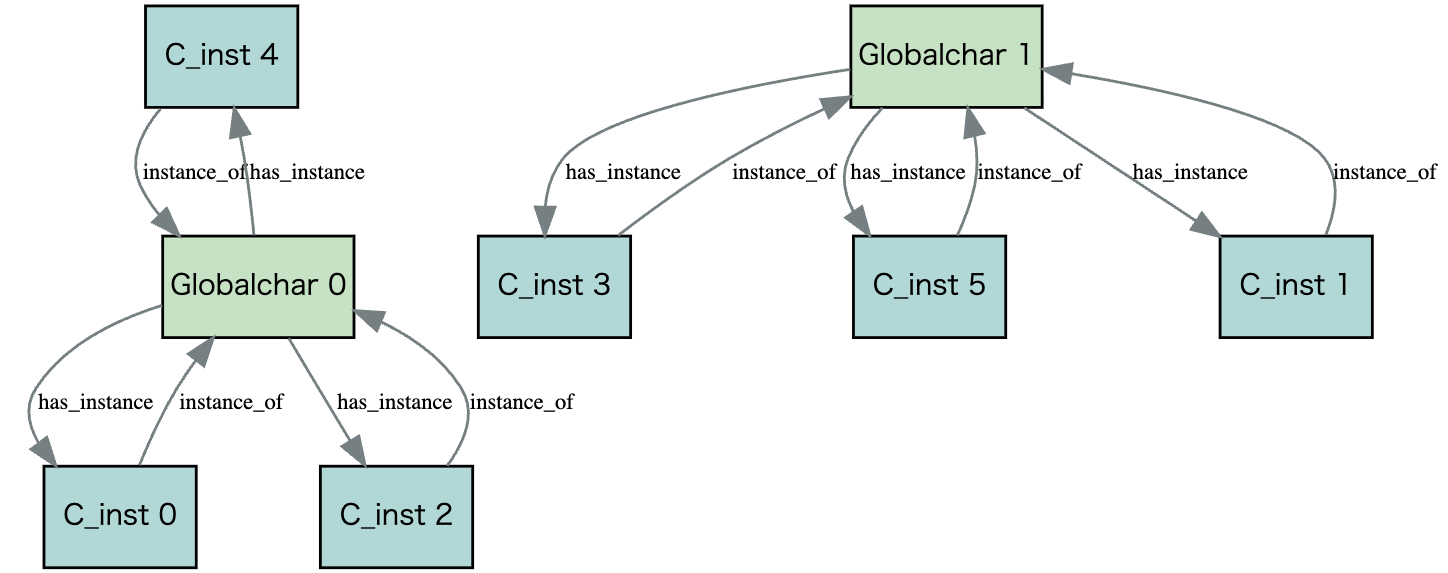
\includegraphics[width=\textwidth]{pict/05/samples_character_edge.png}
   \caption{CharacterInstanceとCharacterNode間の参照関係の例．C\_instはCharacterInstanceノードを表し，GlobalcharはCharacterノードを表す．}
   \label{fig:sample_character_edge}
\end{figure}
\begin{figure}[p]
   \centering
   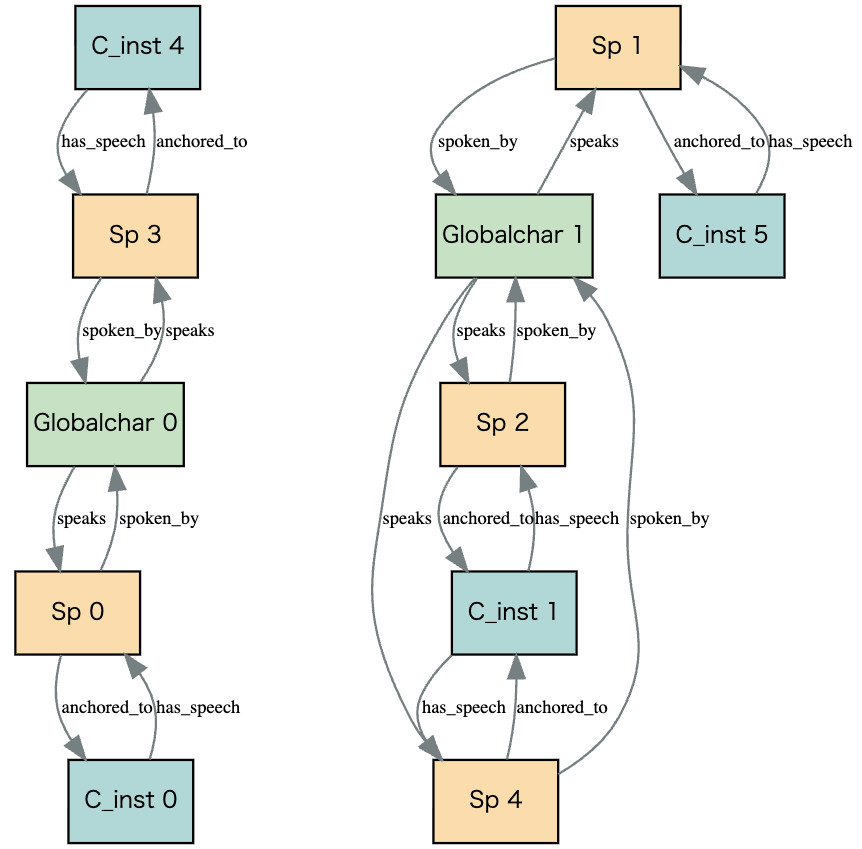
\includegraphics[width=0.7\textwidth]{pict/05/samples_speech_edge.png}
   \caption{SpeechとCharacter Instance および Character を結ぶ参照関係の例．C\_instはCharacterInstanceノードを表し，SpはSpeechノードを，GlobalcharはCharacterノードを表す．}
   \label{fig:sample_speech_edge}
\end{figure}

% ▼▼▼ 仕掛け：main じゃないとき（単体のとき）だけ参考文献を表示 ▼▼▼
\ifdefined\ismain\else
   \printbibliography[title=参考文献]
\fi
% ▲▲▲▲▲▲▲▲▲▲▲▲▲▲▲▲▲▲▲▲▲▲▲▲▲▲▲▲▲▲▲▲▲▲▲▲

\end{document}
\documentclass[a4j,12pt,dvipdfmx]{jsreport}

% 数式
\usepackage{amsmath,amsfonts}
\usepackage{bm}

% 画像
\usepackage[dvipdfmx,top=35truemm,bottom=30truemm,left=30truemm,right=30truemm]{geometry}
\usepackage[dvipdfmx]{graphicx}
% biblatex
\usepackage[style=numeric, sorting=none, maxbibnames=1000]{biblatex}
\addbibresource{graduation_thesis.bib}

% itembox
\usepackage{ascmac}
% breakitemboxのためのpackage
\usepackage{itembkbx}
% \usepackage{tcolorbox} 画像が見えなくなってしまう原因
% \usepackage{framed} 枠

% フォント
\usepackage[ipaex]{pxchfon}
\listfiles
\usepackage{float}
\usepackage{multicol}
\usepackage{multirow}
\usepackage{paralist}
\usepackage{caption}
% \captionsetup{format=plain, justification=centering}
\usepackage{setspace}
\usepackage{algorithm}
\usepackage{algpseudocode}
\usepackage[dvipdfmx,hidelinks]{hyperref}
\usepackage{pxjahyper}
\usepackage{fancyhdr}
\usepackage{ltablex}
\usepackage{capt-of}
\usepackage{tabularx}
\usepackage[export]{adjustbox}
\usepackage{booktabs}
\usepackage{enumitem} % itemizeの行間 これは下になければならない
\usepackage{threeparttable} % 表の脚注
\usepackage{titlesec}
\usepackage{makecell}
\usepackage{forest}
\usepackage{fancybox}
\usepackage{longtable}
\usepackage{xltabular}
% titlesec と \paragraph の相性問題を回避（run-in 見出しにする）
\titleformat{\paragraph}[runin]
  {\normalfont\normalsize\bfseries}
  {}{0pt}{} % ←ここには文字や \noindent 等を入れない
\titlespacing*{\paragraph}
  {0pt}{1.0ex}{0.8em}
\titleformat{\chapter}[hang]{\LARGE\bfseries}{\prechaptername\thechapter\postchaptername}{1em}{}

\setlength{\headheight}{16.5pt}
\captionsetup{format=hang}
\captionsetup[figure]{font=small}
\captionsetup[table]{font=small}
\begin{document}

% ▼▼▼ 仕掛け：main じゃないとき（単体のとき）だけヘッダー設定 ▼▼▼
\ifdefined\ismain\else
   \pagestyle{fancy}
   \lhead{\rightmark}
   \renewcommand{\chaptermark}[1]{\markboth{第\ \thechapter\ 章\ #1}{}}
   \setlength{\headheight}{16.5pt}
   \titleformat{\chapter}[hang]{\LARGE\bfseries}{\prechaptername\thechapter\postchaptername}{1em}{}
\fi
% ▲▲▲▲▲▲▲▲▲▲▲▲▲▲▲▲▲▲▲▲▲▲▲▲▲▲▲▲▲▲▲▲▲▲▲▲
\chapter{脚本に基づく漫画のネーム生成}
\label{chap:script2name}
本章では，構築したManga109NameDataset を用いて，
脚本に基づき漫画のネームを生成する手法について述べる．

本研究では，
ネームを，要素の幾何学的な配置を表すレイアウト情報（Layout）と
演出情報（Direction）が統合された，
物語と作品とを結ぶ中間表現として定義する．
Manga109NameDataset は，
この定義に基づき，
漫画画像に由来するネーム情報を
構造化データとして整理・構築したものである．

第~\ref{chap:script2layout}章で扱った脚本に基づくレイアウト生成では，
物語内容がコマや要素の配置にどのように反映されるかに着目していた．
これに対し本章では，Manga109NameDatasetを用いて
配置そのものに加え，
カメラワークやキャラクターの感情，
場面の雰囲気といった演出情報を含む
より包括的なネーム生成を対象とする．

すなわち本研究では，
脚本（Script）を入力とし，
演出情報（Direction）および
レイアウト情報（Layout）を生成することで，
脚本からネームへ至る生成過程を
計算機上で明示的に扱うことを目的とする．

本章の構成は以下の通りである．
まず~\ref{sec:script2name_formulation}節では，
脚本・演出情報・レイアウト情報からなる
ネーム生成タスクの問題設定を整理し，
定式化を行う．
次に~\ref{sec:script2name_method}節において，
脚本からネームを生成するための手法の概要を述べ，
演出情報およびレイアウト情報をどのように扱うかを説明する．
~\ref{sec:script2name_experiment}節では，
実験設定および評価方法について述べ，
最後に~\ref{sec:script2name_results}節で，
定量的および定性的な評価結果を示し，
脚本に基づくネーム生成の有効性について考察する．

\section{漫画のネーム生成における問題設定}
\label{sec:script2name_formulation}
本節では，
本研究における漫画のネーム生成タスクの問題設定を整理する．
特に，
脚本（Script）・演出情報（Direction）・レイアウト情報（Layout）からなる
三層構造の観点から，
本研究が対象とする生成問題を
脚本（Script）を入力とし，
演出情報（Direction）およびレイアウト情報（Layout）を生成する問題として定式化する． 図\ref{fig:script2name_formulation}にその概略図を示す．

\begin{figure}[htbp]
   \centering
   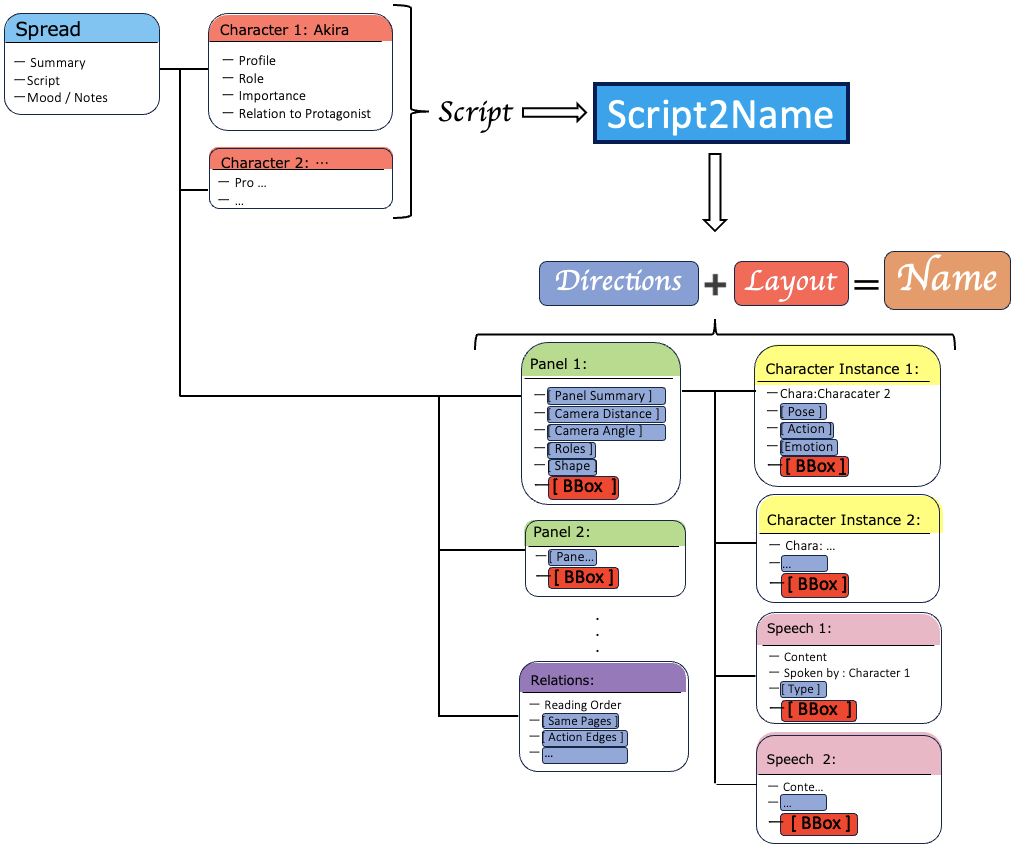
\includegraphics[width=\textwidth]{pict/06/script2name_formulation.png}
   \caption{脚本に基づく漫画ネーム生成タスクの概略図}
   \label{fig:script2name_formulation}
\end{figure}

\subsection{ネーム表現の定義}

本研究では，
第~\ref{chap:script2layout}章第~\ref{sec:problem_formulation}節で述べた
レイアウト表現を拡張し，
漫画のネームを，
$N \in \mathbb{N}$ 個の構成要素と，
場面全体に関わる演出情報からなる表現として定義する．
具体的には，
ネーム $n$ を
\[
   n = \left(
   \mathbf{d}^{\mathrm{global}},
   \{(c_1, \mathbf{d}_1, \mathbf{b}_1), \dots, (c_N, \mathbf{d}_N, \mathbf{b}_N)\}
   \right)
\]
と定義する．

ここで $c_i$ は $i$ 番目の要素のカテゴリを表し，
$\mathbf{d}_i$ はその要素に対応する局所的な演出情報，
$\mathbf{b}_i$ はページ平面上における位置と大きさを表す
バウンディングボックスである．
また，
$\mathbf{d}^{\mathrm{global}}$ は，
見開き全体や場面単位で共有される
グローバルな演出情報を表す．

カテゴリ $c_i$ は，
コマ，キャラクター，セリフといった
基本要素種別に基づくカテゴリ集合 $\mathcal{C}$ の要素であり，
$\mathcal{C}$ は
\[
   \mathcal{C}
   =
   \{\text{panel}\}
   \;\cup\;
   \{\text{character}_k\}
   \;\cup\;
   \{\text{speech}_k\}
\]
として定義される．

局所的な演出情報 $\mathbf{d}_i$ には，
キャラクターの姿勢や感情，
カメラ距離やアングルといった
要素単位で定義される演出属性が含まれる．
一方，
グローバルな演出情報 $\mathbf{d}^{\mathrm{global}}$ には，
主にノード間の関係において現れるエッジ情報
に紐づく演出情報が含まれる．
レイアウト情報 $\mathbf{b}_i$ は，
各要素のページ上での配置を表す
幾何学的情報である．

\subsection{ネーム生成タスクの定式化}

以上の定義のもと，
本研究におけるネーム生成タスクは，
脚本情報 $s$ が与えられたとき，
対応するネーム $n$ を生成する
条件付き生成問題として定式化される．
すなわち，
\[
   f : s
   \;\mapsto\;
   \left(
   \mathbf{d}^{\mathrm{global}},
   \{(c_i, \mathbf{d}_i, \mathbf{b}_i)\}_{i=1}^{N}
   \right)
\]
を学習することが目的である．

第~\ref{chap:script2layout}章で扱った
脚本に基づくレイアウト生成では，
$\mathbf{b}_i$ のみを生成対象としていたのに対し，
本章では，
局所的およびグローバルな演出情報 $\mathbf{d}_i$，
$\mathbf{d}^{\mathrm{global}}$ と
レイアウト情報 $\mathbf{b}_i$ を
統合的に生成する点が異なる．
これにより，
脚本に含まれる物語的文脈が，
配置設計だけでなく，
場面全体および要素単位の演出上の意思決定に
どのように反映されるかを
明示的に扱うことが可能となる．

\section{脚本に基づく漫画のネーム生成手法}
\label{sec:script2name_method}

本節では，
前節で定式化した脚本に基づく漫画のネーム生成タスクに対し，
本研究で用いた生成手法の概要を述べる．
本研究では，
脚本（Script）を入力とし，
演出情報（Direction）および
レイアウト情報（Layout）を
自然言語系列として出力する
LLM に基づくネーム生成手法を構築した．

基本的な枠組みは，
第~\ref{chap:script2layout}章で述べた
脚本に基づくレイアウト生成手法と同様に，
LLMを
教師あり学習によりファインチューニングするものである．
すなわち，
脚本表現をトークン列として入力し，
対応するネーム表現を
自己回帰的に出力するモデルを構築した．

入力となる脚本 $S$ は，
柱，ト書き，およびセリフを含む
見開き単位の脚本全文に加え，
脚本に登場するキャラクターの
プロフィールや役割といった
キャラクター設定を含む
自然言語列として与えられる．
これにより，
モデルは物語の進行だけでなく，
キャラクターの性格や立場といった
文脈情報を条件として利用できる．

ネーム生成においては，
LLM による生成および学習を可能にするため，
入力および出力を
あらかじめ定めた JSON 形式に基づいて線形化し，
トークン列として表現する．

具体的には，
ネームの構造を表す JSON テンプレートを事前に定義し，
コマ，キャラクターインスタンス，セリフといった
各要素に対応するフィールドを所定の位置に配置する．
モデルは，
このテンプレート構造を条件として，
演出情報（Direction）および
レイアウト情報（Layout）に対応するフィールドを
逐次生成する．

このとき，
ネームを構成する要素集合
$\{(c_i, \mathbf{d}_i, \mathbf{b}_i)\}_{i=1}^{N}$ は，
JSON 構造に沿って列挙され，
系列
\[
   \mathcal{N} = (\nu_1, \nu_2, \dots, \nu_T)
\]
として表現される．
各トークン $\nu_t$ は，
単一の要素に対応する
\[
   \nu_t = (c_{\pi(t)}, \mathbf{d}_{\pi(t)}, \mathbf{b}_{\pi(t)})
\]
として定義され，
$\pi(t)$ は
ネームを構成する全要素を
一度ずつ列挙する写像である．

演出情報 $\mathbf{d}_i$ は，
キャラクターの姿勢や感情，
カメラ距離やアングル，
コマの役割といった
要素単位で定義される演出属性の集合であり，
自然言語または離散的な記号列として表現される．
また，
見開き全体や場面単位で共有される
グローバルな演出情報
$\mathbf{d}^{\mathrm{global}}$ についても，
同様に JSON テンプレート内の所定の位置に配置し，
系列生成の一部として扱う．

レイアウト情報 $\mathbf{b}_i$ は，
各要素のページ平面上での位置と大きさを表す
バウンディングボックス
$\mathbf{b}_i = (x_i, y_i, w_i, h_i)$ として定義され，
脚本に基づくレイアウト生成と同様に，
あらかじめ定義した格子上に量子化された
離散トークンとして出力される．

学習時には，漫画のレイアウト生成手法と同様に，
脚本列 $S$ と，
それに対応する正解ネーム列 $\mathcal{N}$ からなる
教師データを用い，
LLM による条件付き確率
\[
   p_{\theta}(\mathcal{N} \mid S)
   =
   \prod_{t=1}^{T}
   p_{\theta}(\nu_t \mid \nu_{<t}, S)
\]
を最大化するように，
モデルパラメータ $\theta$ を最適化する．
損失関数としては，
次トークン予測に基づく
クロスエントロピー損失を用いる．

以上のように，
本研究では，
キャラクター設定を含む脚本を入力とし，
演出情報およびレイアウト情報を
構造化された形式で生成することで，
物語内容と演出設計とを統合した
ネーム生成を，
LLM による条件付き系列生成として実現する．

\section{漫画のネーム生成における実験設定}
\label{sec:script2name_experiment}
本節では，
脚本に基づくネーム生成手法の有効性を検証するために行った
実験設定について述べる．
具体的には，
実験に用いた Manga109NameDataset に含まれる
脚本（Script），演出情報（Direction），レイアウト情報（Layout）の構成を整理した上で，
これらの情報をどのように入力・出力として扱うかを定義する生成設定を説明する．
さらに，
データセット分割，
比較に用いたモデル，
学習および実装条件，
ならびに評価方法について順に述べる．

\subsection{データセットと入力・出力の整理}

本研究では，
脚本からネームを生成する過程を扱うにあたり，
まずデータセット内に含まれる情報を，
脚本（Script），演出情報（Direction），
およびレイアウト情報（Layout）という
三層構造の観点から整理する．
これは，
どの情報を入力として与え，
どの情報を生成対象とするかを
明確に定義するための前提となる．

Manga109NameDataset に含まれる主要なノードおよび属性を，
この三層構造に基づいて分類した結果を
表~\ref{tab:sdl_mapping} に示す．
Script 層には，
見開き全体の脚本本文に加え，
登場キャラクターのプロフィールや役割といった
グローバルな物語文脈に関わる情報が含まれる．
Direction 層には，
各コマやキャラクターインスタンスに対応する
演出上の意思決定を表す属性，
ならびにコマ間・キャラクター間の関係を表す
構造的情報が含まれる．
Layout 層は，
これらの要素がページ平面上で
どの位置・大きさに配置されるかを表す
幾何学的情報から構成される．

\begin{xltabular}{\textwidth}{ll >{\raggedright\arraybackslash}p{4.0cm} >{\small}X}

   % --- 最初のページのヘッダー ---
   \caption{Manga109NameDataset におけるScript/Direction/Layout構成の整理} \label{tab:sdl_mapping} \\
   \toprule
   \textbf{層} & \textbf{ノード} & \textbf{フィールド} & \textbf{内容} \\
   \midrule
   \endfirsthead

   % --- 2ページ目以降のヘッダー ---
   \caption[]{Manga109NameDataset における主要フィールドの構成（続き）} \\
   \toprule
   \textbf{層} & \textbf{ノード} & \textbf{フィールド} & \textbf{内容} \\
   \midrule
   \endhead

   % --- フッター（次ページへ続く...） ---
   \bottomrule
   \multicolumn{4}{r}{\small\textit{次ページへ続く...}} \\
   \endfoot

   % --- 最終フッター ---
   \bottomrule
   \endlastfoot

   % --- データ本体 ---
   \multirow{7}{*}{Script}
   & Spread
   & summary, script, \newline mood, notes
   & 見開き全体の要約・脚本（柱/ト書き/セリフ）・雰囲気・補足 \\
   \addlinespace
   & Character
   & name, profile, role, \newline importance, alignment, \newline \texttt{relation\_to\_protagonist}
   & キャラクター設定（プロフィール、役割、重要度、主人公との関係など） \\
   \addlinespace
   & Speech
   & text, \texttt{speaker\_id}
   & セリフ本文と話者識別ID \\
   \addlinespace
   & Structure
   & \texttt{panel\_ids}
   & 脚本中で言及されるパネルID列 \\
   \midrule
   \multirow{15}{*}{Direction}
   & Panel
   & summary
   & 各コマの内容要約（視覚的説明） \\
   & Panel
   & \texttt{roles} (categorical)
   & コマの役割（dialogue, reaction等） \\
   & Panel
   & \texttt{shape\_type}
   & コマ形状（standard, inset等） \\
   & Panel
   & \texttt{cinematic.distance}, \newline \texttt{cinematic.angle}
   & カメラ距離・アングル \\
   \addlinespace
   & Char. Inst.
   & pose, action, emotion
   & 姿勢・動作・感情（自由記述テキスト） \\
   & Char. Inst.
   & \texttt{pose}, \texttt{action}, \newline \texttt{emotion}, \texttt{face\_body} \newline (all categorical)
   & 姿勢・動作・感情・描写範囲（離散カテゴリ） \\
   \addlinespace
   & Speech
   & \texttt{type} (categorical)
   & セリフ種別（dialogue, monologue等） \\
   \addlinespace
   & Edges
   & \texttt{panel\_edges}
   & コマ間関係（順序や同一ページ判定） \\
   & Edges
   & \texttt{action\_edges}
   & キャラクター間相互作用（source/target/action） \\
   & Edges
   & \texttt{anchored\_to}
   & セリフのアンカー（Speech $\to$ Character） \\
   & Edges
   & \texttt{contains} (pred.)
   & Panel $\to$ Speech/Character の包含関係（予測） \\
   \midrule
   \multirow{5}{*}{Layout}
   & Panel
   & \texttt{bbox}
   & バウンディングボックス $\mathbf{b}_i=(x,y,w,h)$ \\
   & Char. Inst.
   & \texttt{bbox}
   & 同上（キャラクター位置） \\
   & Speech
   & \texttt{bbox}
   & 同上（セリフ位置） \\

\end{xltabular}

このように Script / Direction / Layout を整理した上で，
本研究では，
脚本からネームを生成する際の
情報生成の関係性を検証するため，
入力と出力の組み合わせが異なる
複数の生成設定を比較した．
表~\ref{tab:script2name_settings} に，
本研究で検討した 4 つの生成設定を示す．
これらの設定は，
脚本のみを入力としてレイアウトを生成する設定から，
演出情報とレイアウトを同時に生成する設定，
さらに演出情報を中間表現として経由する
段階的生成設定まで，
ネーム生成における生成粒度と生成順序が
異なる点で区別される．
特に，
Script2Name (Joint) は
演出情報とレイアウト情報を統合的に生成する設定であり，
Script2Direction2Layout は
演出情報を明示的な中間表現として導入することで，
段階的生成の有効性を検証するための設定である．

\begin{table}[htbp]
   \centering
   \caption{脚本に基づくネーム生成の比較設定．GNNはGraphical Neural Networkを表す．}
   \label{tab:script2name_settings}

   % 1. 文字サイズを小さくする (small より小さい footnotesize も検討)
   \small

   % 2. 列間隔を詰める (標準は6pt。ここでは3ptに半減)
   \setlength{\tabcolsep}{3pt}

   \begin{tabular}{lccc}
      \toprule
      \textbf{設定名} & \textbf{入力}                    & \textbf{出力} & \textbf{モデル構成} \\
      \midrule
      Script2Layout
                   & Script
                   & Layout
                   & LLM                                                           \\
      \addlinespace
      Script2Name (Joint)
                   & Script
                   & Direction + Layout
                   & LLM                                                           \\
      \addlinespace
      (Script+Direction)2Layout
                   & Script + Direction
                   & Layout
                   & LLM                                                           \\
      \addlinespace
      Script2Direction2Layout
                   & Script
                   & Direction $\rightarrow$ Layout
                   & LLM + GNN                                                     \\
      \bottomrule
   \end{tabular}
\end{table}



本研究では，これらの設定に基づき，
脚本からネーム生成へ至る過程を
異なる情報分解および生成順序の観点から比較する．
これらの生成設定は，
実際の漫画制作において，
演出を先に検討する場合や，
配置設計と演出を同時に検討する場合など，
制作工程や作家の作業スタイルに応じて
ネームの設計手順が異なる状況を抽象化したものである．
このような複数の生成設定を通じて，
脚本からネームを構築する際に，
演出情報をどの段階でどのように扱うことが有効であるかを
体系的に検証する．

\subsection{データセット分割}
学習に用いたManga109NameDatasetは，作品単位で分割し，
同一作品が訓練用・検証用・テスト用データにまたがらないようにした．
分割比は 8:1:1
訓練用データ 7{,}937 見開き，
検証用データ 1{,}113 見開き，
テスト用データ 991 見開きを用いた．

訓練用データは各生成設定におけるモデルの学習に，
検証用データは学習の早期終了およびモデル選択に用い，
最終的な性能評価はテスト用データ上で行った．
なお，
データセット分割および前処理の方針は，
第~\ref{chap:script2layout}章のレイアウト生成実験と同一である．

\subsection{比較手法}
脚本に基づくネーム生成手法の有効性の検証においても
第~\ref{chap:script2layout}章のレイアウト生成実験と同様，
既存のレイアウト生成手法との比較を行った．
比較に用いた手法も同じく，
LayoutDM~\cite{inoue2023layoutdm}，
LayoutFormer++~\cite{jiang_layoutformer_2023}，
LayoutPrompter~\cite{lin_layoutprompter_2023}
の 3 手法である．
これらの既存手法は，
ネーム生成における比較においても，要素カテゴリ情報を入力条件として与える Gen-T条件での生成に用い，脚本を条件とする生成条件にあわせてレイアウト生成性能の比較に用いた．

ほか学習の設定や推論の設定は，グリッド条件を見開き単位に対応させることを除いて第~\ref{chap:script2layout}章のレイアウト生成実験と同様である．

\subsection{ネーム生成における学習設定および実装詳細}
本節では，
表~\ref{tab:script2name_settings} に示した各生成設定において用いた
モデル構成と学習条件，ならびに実装上の設定について述べる．
LLM による生成設定である Script2Layout / Script2Name (Joint) / (Script+Direction)2Layout では，
教師ありファインチューニングを行った．
一方，段階的生成設定 Script2Direction2Layout では，
演出情報の生成に LLM をファインチューニングし，
レイアウト生成にはグラフニューラルネットワーク（GNN）を用いた．

\paragraph{LLM の選定}
本実験では，LLM として \texttt{gpt-oss-20b}，\texttt{Qwen3-14B}，\texttt{Llama-3.1-8B} を選定した．
これらはいずれも公開モデルの中で比較的新しく，
汎用的な言語能力において高い評価を得ていることから採用した．
複数の基盤モデルを用いることで，
モデル規模や事前学習の差異がネーム生成性能に与える影響を検証した．
学習は，各見開きの脚本（および条件に応じて演出情報）を入力とし，
JSON 形式に線形化した出力列を教師信号として，
次トークン予測に基づくクロスエントロピー損失を最小化することで行った．
学習手順は，第~\ref{chap:script2layout}章のレイアウト生成と同様である．

\paragraph{GNN によるレイアウト生成（Script2Direction2Layout）}
段階的生成設定 Script2Direction2Layout では，
まず LLM により脚本から演出情報（Direction）を生成し，
得られた Direction を条件として
GNN によりレイアウト（BBox）を推定した．
GNN は，見開きを表す異種グラフを入力とする HeteroConv に基づくモデルとして実装し，
ノード種別は Spread / Panel / Character / Character Instance / Speech とした．
エッジには，キャラクターインスタンス間の相互作用（action edges），
Panel と Character Instance の包含関係，
Speech の読順関係など，
Manga109NameDataset に含まれる主要な関係情報を用いた．
各ノードには，対応するテキスト特徴および演出属性を付与し，
メッセージパッシングによって特徴を更新した後，
Panel，CharacterInstance，Speech の各ノードに対して
混合密度ネットワーク（MDN）を用いてバウンディングボックスを推定した．

\paragraph{レイアウト表現の量子化と座標系}
レイアウト情報は，
各要素のバウンディングボックス
$\mathbf{b}_i = (x_i, y_i, w_i, h_i)$
として表現される．
LLM および GNN による生成を可能にするため，
これらの連続値座標は，
あらかじめ定義した格子上に量子化された
離散トークンとして扱った．

第~\ref{chap:script2layout}章のレイアウト生成では
ページ単位の生成を対象としていたため，
座標系を $32 \times 32$ の格子として定義していたのに対し，
本章では見開き単位のネーム生成を扱うことから，
横方向の表現範囲を拡張し，
$64 \times 32$ の格子を用いた．
これにより，
見開き全体を一貫した座標系で表現しつつ，
既存のレイアウト生成手法との整合性を保った．

\subsection{評価方法}
本研究では，
脚本に基づくネーム生成手法の有効性を検証するため，
主としてレイアウト生成結果に対する定量評価を行った．
レイアウトに関する評価指標および評価手順は，
第~\ref{chap:script2layout}章で用いたものと同一であり，
mIoU，FID，LTSim，LTSim-MMD を用いた．
これらの指標により，
要素の位置や大きさといった
幾何的配置の再現性を，
正解レイアウトとの比較に基づいて評価した．
そのため，
本章では各評価指標の詳細な定義については省略する．

一方で，
演出情報（Direction）については，
直接的な定量評価は行っていない．
これは，
Direction がカメラワーク，感情表現，場面の雰囲気といった
高次の意味的・主観的要素を含むため，
単一の数値指標として妥当な正解度を定義することが
現時点では困難であるためである．

そこで本研究では，
演出情報の生成結果について，
二つの観点から評価を行った．
第一に，
生成された Direction を
ノードおよび関係からなるグラフ構造として可視化し，
対応する正解データと比較することで，
キャラクター配置関係や
演出上の役割分担が
脚本内容と整合しているかを
定性的に分析した．

第二に，
段階的生成設定 Script2Direction2Layout においては，
Direction を入力としてレイアウトを生成する
グラフニューラルネットワーク（GNN）を評価器として用い，
生成された Direction の妥当性を
間接的に評価した．
具体的には，
同一の GNN に対して，
正解 Direction および
LLM により生成された Direction をそれぞれ入力し，
得られたレイアウト結果を
正解レイアウトと比較することで，
Direction がレイアウト生成に提供する
構造的情報の再現性を評価した．
この評価は，
Direction の意味内容そのものを直接測定するものではないが，
下流タスクであるレイアウト生成に対して
どの程度有効な情報を保持しているかを
定量的に比較するための指標として位置づけられる．

以上の評価方法により，
本研究では，
ネーム生成における
レイアウトの幾何的再現性と，
演出情報の構造的妥当性の双方について，
定量的および定性的な観点から分析を行った．
演出情報に対する
より直接的な定量評価指標の設計については，
今後の課題とする．

\section{漫画のネーム生成における結果と考察}\label{sec:script2name_results}
本節では，
前節で述べた各生成設定に基づく実験結果をもとに，
脚本に基づくネーム生成における
レイアウト生成性能および
生成設定の違いが与える影響について考察する．
特に，
既存のレイアウト生成手法との比較，
LLM に基づく各生成設定の傾向，
演出情報の統合方法の違い，
および段階的生成における課題の観点から結果に付いて考察する．

\subsection{漫画のネーム生成における定量的結果と考察}
表~\ref{tab:script2name_results_layout} に，ネーム生成におけるレイアウト生成性能の定量的結果を示す．

\begin{table*}[t]
   \captionsetup{font=small}
   \caption{
      脚本に基づくネーム生成におけるレイアウト生成の定量評価結果（見開き単位）．
   }
   \vspace{-0.6em}
   \centering
   \label{tab:script2name_results_layout}
   \setlength{\tabcolsep}{6pt}
   \begin{adjustbox}{max width=\textwidth}
      \begin{tabular}{l c c c c}
         \toprule
                                                           &
         \multicolumn{2}{c}{\textbf{Spread-level metrics}} &
         \multicolumn{2}{c}{\textbf{Distribution-level metrics}}                                                                                                              \\
         \cmidrule(lr){2-3} \cmidrule(lr){4-5}
         \textbf{Model}                                    &
         mIoU $\uparrow$                                   & LTSim $\uparrow$                                    &
         FID $\downarrow$                                  & \makecell{LTSim-MMD ($\times 10^{-2}$)$\downarrow$}                                                              \\
         \midrule

         \multicolumn{5}{l}{\itshape Existing layout generation methods (Category-conditioned)}                                                                               \\

         LayoutDM
                                                           & 0.0989                                              & 0.7064             & 54.095            & \underline{0.645} \\
         LayoutFormer++
                                                           & 0.0325                                              & 0.5632             & 56.520            & 5.258             \\
         LayoutPrompter
                                                           & 0.0964                                              & 0.6739             & 64.941            & 1.912             \\
         \midrule

         \multicolumn{5}{l}{\itshape Script2Direction2Layout (Fine-tuned LLM $\rightarrow$ GNN)}                                                                              \\

         GPT-OSS-20B
                                                           & 0.0851                                              & 0.7123             & 78.45             & 2.19              \\
         Llama-3.1-8B
                                                           & 0.0772                                              & 0.7055             & 105.10            & 3.75              \\
         Qwen3-14B
                                                           & 0.0822                                              & 0.7106             & 74.97             & 2.35              \\
         \midrule

         \multicolumn{5}{l}{\itshape (Script + Direction) $\rightarrow$ Layout (Fine-tuned LLM)}                                                                              \\

         GPT-OSS-20B
                                                           & 0.1086                                              & \underline{0.7484} & 14.52             & 0.71              \\
         Llama-3.1-8B
                                                           & 0.0162                                              & 0.4212             & 165.30            & 64.17             \\
         Qwen3-14B
                                                           & 0.1178                                              & \textbf{0.7711}    & \textbf{9.21}     & \textbf{0.50}     \\
         \midrule

         \multicolumn{5}{l}{\itshape Script $\rightarrow$ (Direction + Layout) (Fine-tuned LLM, Joint)}                                                                       \\

         GPT-OSS-20B
                                                           & \underline{0.1201}                                  & 0.7360             & 19.76             & 1.04              \\
         Llama-3.1-8B
                                                           & 0.0140                                              & 0.4154             & 168.78            & 64.68             \\
         Qwen3-14B
                                                           & 0.1254                                              & 0.7434             & 19.72             & 0.90              \\
         \midrule

         \multicolumn{5}{l}{\itshape Script2Layout (Fine-tuned LLM)}                                                                                                          \\

         GPT-OSS-20B
                                                           & 0.1177                                              & 0.7333             & 18.88             & 1.24              \\
         Llama-3.1-8B
                                                           & 0.0142                                              & 0.4165             & 166.84            & 64.06             \\
         Qwen3-14B
                                                           & \textbf{0.1269}                                     & 0.7421             & \underline{18.72} & 0.87              \\
         \bottomrule
      \end{tabular}
   \end{adjustbox}
\end{table*}


\paragraph{既存レイアウト生成手法との比較}

\paragraph{LLM に基づくネーム生成手法の全体的傾向}
...

\paragraph{演出情報の統合方法による違い}
...

\paragraph{段階的生成（Script2Direction2Layout）の限界}

% ▼▼▼ 仕掛け：main じゃないとき（単体のとき）だけ参考文献を表示 ▼▼▼
\ifdefined\ismain\else
   \printbibliography[title=参考文献]
\fi
% ▲▲▲▲▲▲▲▲▲▲▲▲▲▲▲▲▲▲▲▲▲▲▲▲▲▲▲▲▲▲▲▲▲▲▲▲

\end{document}
\documentclass[a4j,12pt,dvipdfmx]{jsreport}

% 数式
\usepackage{amsmath,amsfonts}
\usepackage{bm}

% 画像
\usepackage[dvipdfmx,top=35truemm,bottom=30truemm,left=30truemm,right=30truemm]{geometry}
\usepackage[dvipdfmx]{graphicx}
% biblatex
\usepackage[style=numeric, sorting=none, maxbibnames=1000]{biblatex}
\addbibresource{graduation_thesis.bib}

% itembox
\usepackage{ascmac}
% breakitemboxのためのpackage
\usepackage{itembkbx}
% \usepackage{tcolorbox} 画像が見えなくなってしまう原因
% \usepackage{framed} 枠

% フォント
\usepackage[ipaex]{pxchfon}
\listfiles
\usepackage{float}
\usepackage{multicol}
\usepackage{multirow}
\usepackage{paralist}
\usepackage{caption}
% \captionsetup{format=plain, justification=centering}
\usepackage{setspace}
\usepackage{algorithm}
\usepackage{algpseudocode}
\usepackage[dvipdfmx,hidelinks]{hyperref}
\usepackage{pxjahyper}
\usepackage{fancyhdr}
\usepackage{ltablex}
\usepackage{capt-of}
\usepackage{tabularx}
\usepackage[export]{adjustbox}
\usepackage{booktabs}
\usepackage{enumitem} % itemizeの行間 これは下になければならない
\usepackage{threeparttable} % 表の脚注
\usepackage{titlesec}
\usepackage{makecell}
\usepackage{forest}
\usepackage{fancybox}
% titlesec と \paragraph の相性問題を回避（run-in 見出しにする）
\titleformat{\paragraph}[runin]
  {\normalfont\normalsize\bfseries}
  {}{0pt}{} % ←ここには文字や \noindent 等を入れない
\titlespacing*{\paragraph}
  {0pt}{1.0ex}{0.8em}
\titleformat{\chapter}[hang]{\LARGE\bfseries}{\prechaptername\thechapter\postchaptername}{1em}{}

\setlength{\headheight}{16.5pt}
\captionsetup{format=hang}
\captionsetup[figure]{font=small}
\captionsetup[table]{font=small}
\begin{document}

% ▼▼▼ 仕掛け：main じゃないとき（単体のとき）だけヘッダー設定 ▼▼▼
\ifdefined\ismain\else
   \pagestyle{fancy}
   \lhead{\rightmark}
   \renewcommand{\chaptermark}[1]{\markboth{第\ \thechapter\ 章\ #1}{}}
   \setlength{\headheight}{16.5pt}
   \titleformat{\chapter}[hang]{\LARGE\bfseries}{\prechaptername\thechapter\postchaptername}{1em}{}
\fi
% ▲▲▲▲▲▲▲▲▲▲▲▲▲▲▲▲▲▲▲▲▲▲▲▲▲▲▲▲▲▲▲▲▲▲▲▲

\chapter{結論}\label{chap:conclusion}

本研究では，
漫画制作工程において重要な役割を担う「ネーム」を，
作品の下書き画像そのものではなく，
物語文脈と演出意図を内包した
構造化された中間表現として捉え直し，
脚本に基づく漫画ネーム生成という新たな課題設定を提示した．
従来のレイアウト生成研究が，
主として機能的媒体や要素配置の最適化を対象としてきたのに対し，
本研究は，
物語性や演出上の意思決定と不可分な
漫画特有の配置問題を扱う点に特徴がある．

この課題に取り組むため，
本研究では，
大規模視覚言語モデル（LVLM）を活用し，
漫画画像に紐づく物語情報および演出情報を体系的に抽出・構造化した
Manga109ScriptDataset および Manga109NameDataset を構築した．
特に，
人手による読み順アノテーションと
独自の Visual Prompting 手法を組み合わせることで，
LVLM 単体では困難であった
漫画特有の物語構造や演出情報の記述を可能にし，
脚本およびネーム生成のための学習基盤を整備した．

さらに，
構築したデータセットを用いて，
脚本を入力とし，
演出情報およびレイアウト情報を生成する
漫画ネーム生成モデルを提案した．
大規模言語モデル(LLM)を基盤とした複数の生成設定を比較した結果，
脚本情報を明示的に入力として与えることで，
既存のレイアウト生成手法を上回る性能が得られることを
定量的・定性的に示した．
また，
演出情報をどの段階で統合するかという設計の違いなどを複数検討し設計指針を整理した．

一方で，
演出情報は本質的に多義的であり，
単一の正解に基づく評価が難しいという課題も明らかとなった．
本研究では，
GNN を用いた間接評価や可視化分析を通じて，
演出情報の品質を検討したが，
明らかに文脈と乖離した演出や，
制作上不適切な生成結果を抑制するためには，
演出情報の妥当性や一貫性を
より定量的に捉える評価指標の設計が今後必要である．

脚本を条件としてネームを生成するという枠組みは，
最終成果物を直接生成するのではなく，
制作工程の中核に位置する意思決定を支援するという点で，
創作者の創造性を尊重しつつ，
制作効率の向上に寄与し得る可能性をもつと考えられる．
本研究で示したデータセット，モデル設計，および評価結果は，
脚本に基づく漫画ネーム生成という新たな研究領域における
基礎的なベースラインとなるものであり，
今後の発展的研究や実制作支援への応用に向けた
重要な足がかりとなることを期待する．


% ▼▼▼ 仕掛け：main じゃないとき（単体のとき）だけ参考文献を表示 ▼▼▼
\ifdefined\ismain\else
   \printbibliography[title=参考文献]
\fi
% ▲▲▲▲▲▲▲▲▲▲▲▲▲▲▲▲▲▲▲▲▲▲▲▲▲▲▲▲▲▲▲▲▲▲▲▲

\end{document}
\documentclass[a4j,12pt,dvipdfmx]{jsreport}

% 数式
\usepackage{amsmath,amsfonts}
\usepackage{bm}

% 画像
\usepackage[dvipdfmx,top=35truemm,bottom=30truemm,left=30truemm,right=30truemm]{geometry}
\usepackage[dvipdfmx]{graphicx}
% biblatex
\usepackage[style=numeric, sorting=none, maxbibnames=1000]{biblatex}
\addbibresource{graduation_thesis.bib}

% itembox
\usepackage{ascmac}
% breakitemboxのためのpackage
\usepackage{itembkbx}
% \usepackage{tcolorbox} 画像が見えなくなってしまう原因
% \usepackage{framed} 枠

% フォント
\usepackage[ipaex]{pxchfon}
\listfiles
\usepackage{float}
\usepackage{multicol}
\usepackage{multirow}
\usepackage{paralist}
\usepackage{caption}
% \captionsetup{format=plain, justification=centering}
\usepackage{setspace}
\usepackage{algorithm}
\usepackage{algpseudocode}
\usepackage[dvipdfmx,hidelinks]{hyperref}
\usepackage{pxjahyper}
\usepackage{fancyhdr}
\usepackage{ltablex}
\usepackage{capt-of}
\usepackage{tabularx}
\usepackage[export]{adjustbox}
\usepackage{booktabs}
\usepackage{enumitem} % itemizeの行間 これは下になければならない
\usepackage{threeparttable} % 表の脚注
\usepackage{titlesec}
\usepackage{makecell}
\usepackage{forest}
\usepackage{fancybox}
% titlesec と \paragraph の相性問題を回避（run-in 見出しにする）
\titleformat{\paragraph}[runin]
  {\normalfont\normalsize\bfseries}
  {}{0pt}{} % ←ここには文字や \noindent 等を入れない
\titlespacing*{\paragraph}
  {0pt}{1.0ex}{0.8em}
\titleformat{\chapter}[hang]{\LARGE\bfseries}{\prechaptername\thechapter\postchaptername}{1em}{}

\setlength{\headheight}{16.5pt}
\captionsetup{format=hang}
\captionsetup[figure]{font=small}
\captionsetup[table]{font=small}
\begin{document}

% ▼▼▼ 仕掛け：main じゃないとき（単体のとき）だけヘッダー設定 ▼▼▼
\ifdefined\ismain\else
  \pagestyle{fancy}
  \lhead{\rightmark}
  \renewcommand{\chaptermark}[1]{\markboth{第\ \thechapter\ 章\ #1}{}}
  \setlength{\headheight}{16.5pt}
  \titleformat{\chapter}[hang]{\LARGE\bfseries}{\prechaptername\thechapter\postchaptername}{1em}{}
\fi
% ▲▲▲▲▲▲▲▲▲▲▲▲▲▲▲▲▲▲▲▲▲▲▲▲▲▲▲▲▲▲▲▲▲▲▲▲

\chapter*{謝辞}
\addcontentsline{toc}{chapter}{謝辞}
本研究を行うにあたり，主任指導教員である栗原聡教授には多大なご指導を承りました．橋本敦史訪問准教授，電気通信大学稲葉通将准教授には，研究の指針となるお言葉や技術的な御助言を数多く頂き，また精神的な面においても支えていただきました．心より感謝申し上げます．

本研究は，産業技術総合研究所の覚醒プロジェクトの支援を受けて実施されました．産総研AIセンター社会知能研究チーム長大西正輝先生，唐木田亮先生には，本プロジェクトのPMとして研究を様々な面でご支援頂きました．プロジェクトのメンバーの皆様のお力添えに厚く御礼申し上げます．

栗原研究室の皆様には，研究の面においても生活の面においても大変お世話になりました．特に，畠山太郎氏，北川峻氏，岡田湧路氏，伊藤亮史氏，小菅雷太郎氏には，多くの面でご助力頂きました．心より感謝申し上げます．

最後になりましたが，家族の支えにも感謝いたします．

改めまして，本研究に関わってくださった全ての皆様に心より感謝申し上げます．


% ▼▼▼ 仕掛け：main じゃないとき（単体のとき）だけ参考文献を表示 ▼▼▼
\ifdefined\ismain\else
  \printbibliography[title=参考文献]
\fi
% ▲▲▲▲▲▲▲▲▲▲▲▲▲▲▲▲▲▲▲▲▲▲▲▲▲▲▲▲▲▲▲▲▲▲▲▲

\end{document}

% 参考文献
\fancypagestyle{bibliography}{
   \fancyhead{}
   \fancyhead[RO]{参考文献}
   \cfoot{\thepage}
}
\defbibheading{bibintoc}[\refname]{%
   \chapter*{#1}%
   \markboth{参考文献}{}%
}
\printbibliography[heading=bibintoc, title=参考文献]
\addcontentsline{toc}{chapter}{参考文献}

% 付録
\documentclass[a4j,12pt,dvipdfmx]{jsreport}

% 数式
\usepackage{amsmath,amsfonts}
\usepackage{bm}

% 画像
\usepackage[dvipdfmx,top=35truemm,bottom=30truemm,left=30truemm,right=30truemm]{geometry}
\usepackage[dvipdfmx]{graphicx}
% biblatex
\usepackage[style=numeric, sorting=none, maxbibnames=1000]{biblatex}
\addbibresource{graduation_thesis.bib}

% itembox
\usepackage{ascmac}
% breakitemboxのためのpackage
\usepackage{itembkbx}
% \usepackage{tcolorbox} 画像が見えなくなってしまう原因
% \usepackage{framed} 枠

% フォント
\usepackage[ipaex]{pxchfon}
\listfiles
\usepackage{float}
\usepackage{multicol}
\usepackage{multirow}
\usepackage{paralist}
\usepackage{caption}
% \captionsetup{format=plain, justification=centering}
\usepackage{setspace}
\usepackage{algorithm}
\usepackage{algpseudocode}
\usepackage[dvipdfmx,hidelinks]{hyperref}
\usepackage{pxjahyper}
\usepackage{fancyhdr}
\usepackage{ltablex}
\usepackage{capt-of}
\usepackage{tabularx}
\usepackage[export]{adjustbox}
\usepackage{booktabs}
\usepackage{enumitem} % itemizeの行間 これは下になければならない
\usepackage{threeparttable} % 表の脚注
\usepackage{titlesec}
\usepackage{makecell}
\usepackage{forest}
\usepackage{fancybox}
% titlesec と \paragraph の相性問題を回避（run-in 見出しにする）
\titleformat{\paragraph}[runin]
  {\normalfont\normalsize\bfseries}
  {}{0pt}{} % ←ここには文字や \noindent 等を入れない
\titlespacing*{\paragraph}
  {0pt}{1.0ex}{0.8em}
\titleformat{\chapter}[hang]{\LARGE\bfseries}{\prechaptername\thechapter\postchaptername}{1em}{}

\setlength{\headheight}{16.5pt}
\captionsetup{format=hang}
\captionsetup[figure]{font=small}
\captionsetup[table]{font=small}
\begin{document}

% ▼▼▼ 仕掛け：main じゃないとき（単体のとき）だけヘッダー設定 ▼▼▼
\ifdefined\ismain\else
   \pagestyle{fancy}
   \lhead{\rightmark}
   \renewcommand{\chaptermark}[1]{\markboth{第\ \thechapter\ 章\ #1}{}}
   \setlength{\headheight}{16.5pt}
   \titleformat{\chapter}[hang]{\LARGE\bfseries}{\prechaptername\thechapter\postchaptername}{1em}{}
\fi
% ▲▲▲▲▲▲▲▲▲▲▲▲▲▲▲▲▲▲▲▲▲▲▲▲▲▲▲▲▲▲▲▲▲▲▲▲

\chapter*{研究業績一覧} \label{performance}
\addcontentsline{toc}{chapter}{研究業績一覧}

\section*{国内会議}

\begin{enumerate}[label=(\roman*)]
   \item \textbf{渡邉謙吾}，川村天, 小林伶央, 有井知真, 伊藤亮史, 栗原聡，"物語構造分析に基づくLLMを用いたインタラクティブストーリー生成システム"，第24回データ指向構成マイニングとシミュレーション研究会(SIG-DOCMAS)(人工知能学会合同研究会2023)，Nov.25，2023
   \item 安部玲央, 有井知真, 伊藤亮史, \textbf{渡邉謙吾}, 小林伶央, 川村天, 栗原聡，"アフォーダンスを活用するマルチエージェントプランニングにおけるタスク分解"，第24回 データ指向構成マイニングとシミュレーション研究会(SIG-DOCMAS), Nov.25，2023
\end{enumerate}

% ▼▼▼ 仕掛け：main じゃないとき（単体のとき）だけ参考文献を表示 ▼▼▼
\ifdefined\ismain\else
   \printbibliography[title=参考文献]
\fi
% ▲▲▲▲▲▲▲▲▲▲▲▲▲▲▲▲▲▲▲▲▲▲▲▲▲▲▲▲▲▲▲▲▲▲▲▲

\end{document}

\appendix
\renewcommand{\chaptermark}[1]{\markboth{付録\ \thechapter\ \ #1}{}}
\documentclass[a4j,12pt,dvipdfmx]{jsreport}

% 数式
\usepackage{amsmath,amsfonts}
\usepackage{bm}

% 画像
\usepackage[dvipdfmx,top=35truemm,bottom=30truemm,left=30truemm,right=30truemm]{geometry}
\usepackage[dvipdfmx]{graphicx}
% biblatex
\usepackage[style=numeric, sorting=none, maxbibnames=1000]{biblatex}
\addbibresource{graduation_thesis.bib}

% itembox
\usepackage{ascmac}
% breakitemboxのためのpackage
\usepackage{itembkbx}
% \usepackage{tcolorbox} 画像が見えなくなってしまう原因
% \usepackage{framed} 枠

% フォント
\usepackage[ipaex]{pxchfon}
\listfiles
\usepackage{float}
\usepackage{multicol}
\usepackage{multirow}
\usepackage{paralist}
\usepackage{caption}
% \captionsetup{format=plain, justification=centering}
\usepackage{setspace}
\usepackage{algorithm}
\usepackage{algpseudocode}
\usepackage[dvipdfmx,hidelinks]{hyperref}
\usepackage{pxjahyper}
\usepackage{fancyhdr}
\usepackage{ltablex}
\usepackage{capt-of}
\usepackage{tabularx}
\usepackage[export]{adjustbox}
\usepackage{booktabs}
\usepackage{enumitem} % itemizeの行間 これは下になければならない
\usepackage{threeparttable} % 表の脚注
\usepackage{titlesec}
\usepackage{makecell}
\usepackage{forest}
\usepackage{fancybox}
% titlesec と \paragraph の相性問題を回避（run-in 見出しにする）
\titleformat{\paragraph}[runin]
  {\normalfont\normalsize\bfseries}
  {}{0pt}{} % ←ここには文字や \noindent 等を入れない
\titlespacing*{\paragraph}
  {0pt}{1.0ex}{0.8em}
\titleformat{\chapter}[hang]{\LARGE\bfseries}{\prechaptername\thechapter\postchaptername}{1em}{}

\setlength{\headheight}{16.5pt}
\captionsetup{format=hang}
\captionsetup[figure]{font=small}
\captionsetup[table]{font=small}
\begin{document}

% ▼▼▼ 仕掛け：main じゃないとき（単体のとき）だけヘッダー設定 ▼▼▼
\ifdefined\ismain\else
   \pagestyle{fancy}
   \lhead{\rightmark}
   \renewcommand{\chaptermark}[1]{\markboth{第\ \thechapter\ 章\ #1}{}}
   \setlength{\headheight}{16.5pt}
   \titleformat{\chapter}[hang]{\LARGE\bfseries}{\prechaptername\thechapter\postchaptername}{1em}{}
\fi
% ▲▲▲▲▲▲▲▲▲▲▲▲▲▲▲▲▲▲▲▲▲▲▲▲▲▲▲▲▲▲▲▲▲▲▲▲



% ▼▼▼ 仕掛け：main じゃないとき（単体のとき）だけ参考文献を表示 ▼▼▼
\ifdefined\ismain\else
   \printbibliography[title=参考文献]
\fi
% ▲▲▲▲▲▲▲▲▲▲▲▲▲▲▲▲▲▲▲▲▲▲▲▲▲▲▲▲▲▲▲▲▲▲▲▲

\end{document}


\end{document}